%  ========================================================================
%  Copyright (c) 1985-2014 The University of Washington
%
%  Licensed under the Apache License, Version 2.0 (the "License");
%  you may not use this file except in compliance with the License.
%  You may obtain a copy of the License at
%
%      http://www.apache.org/licenses/LICENSE-2.0
%
%  Unless required by applicable law or agreed to in writing, software
%  distributed under the License is distributed on an "AS IS" BASIS,
%  WITHOUT WARRANTIES OR CONDITIONS OF ANY KIND, either express or implied.
%  See the License for the specific language governing permissions and
%  limitations under the License.
%  ========================================================================
%

% Documentation for University of Washington thesis LaTeX document class
% by Jim Fox
% fox@washington.edu
%
%    Revised for version 2015/03/03 of uwthesis.cls
%
%    This document is contained in a single file ONLY because
%    I wanted to be able to distribute it easily.  A real thesis ought
%    to be contained on many files (e.g., one for each chapter, at least).
%
%    To help you identify the files and sections in this large file
%    I use the string '==========' to identify new files.
%
%    To help you ignore the unusual things I do with this sample document
%    I try to use the notation
%       
%    % --- sample stuff only -----
%    special stuff for my document, but you don't need it in your thesis
%    % --- end-of-sample-stuff ---


%    Printed in twoside style now that that's allowed
%
 
\documentclass [11pt, proquest] {uwthesis}[2015/03/03]
 
%
% The following line would print the thesis in a postscript font 

\usepackage{amsfonts,amsmath,amsthm}
\usepackage[usenames]{color}
\usepackage{mathptmx} % assumes new font selection scheme installed
\usepackage{times} % assumes new font selection scheme installed
\usepackage{amssymb}  % assumes amsmath package installed
\usepackage{tabularx}
\usepackage{graphicx}
\usepackage{dcolumn}
\usepackage{epstopdf}
\usepackage{gensymb}
\usepackage{tikz}
\DeclareGraphicsRule{.eps}{pdf}{.pdf}{`epstopdf #1}
\pdfcompresslevel=9

% Table and figure captions
% http://tex.stackexchange.com/questions/75654/uppercase-until-end-of-group


%\setlength{\oddsidemargin}{0cm} \setlength{\evensidemargin}{0cm}
%\setlength{\topmargin}{-.25cm}  % -2 works for ps but not dvi or pdf!
%\setlength{\textheight}{21.5cm} \setlength{\textwidth}{15.7cm}


% \usepackage{natbib}
% \def\bibpreamble{\protect\addcontentsline{toc}{chapter}{Bibliography}}
\def\checkmark{\tikz\fill[scale=0.4](0,.35) -- (.25,0) -- (1,.7) -- (.25,.15) -- cycle;} 

\setcounter{tocdepth}{1}  % Print the chapter and sections to the toc
 

% ==========   Local defs and mods
%

% --- sample stuff only -----
% These format the sample code in this document

\usepackage{alltt}  % 
\newenvironment{demo}
  {\begin{alltt}\leftskip3em
     \def\\{\ttfamily\char`\\}%
     \def\{{\ttfamily\char`\{}%
     \def\}{\ttfamily\char`\}}}
  {\end{alltt}}
 
% metafont font.  If logo not available, use the second form
%
% \font\mffont=logosl10 scaled\magstep1
\let\mffont=\sf
% --- end-of-sample-stuff ---
 



\begin{document}
 
%% ==========   Preliminary pages
%%
%% ( revised 2012 for electronic submission )
%%
%
%\prelimpages
% 
%%
%% ----- copyright and title pages
%%
%\Title{A Study on the Bike Volume Prediction\\
%  using EcoCounter in Seattle}
%\Author{Weiran Zhao}
%\Year{2016}
%\Program{UW Master of Urban planning}
%
%\Chair{Name of Chairperson}{Title of Chair}{Department of Chair}
%\Signature{First committee member}
%\Signature{Next committee member}
%\Signature{etc}
%
%\copyrightpage
%
%% \titlepage  
%
%% --- sample stuff only -----
%% unusual footnote not found in a real thesis
%% You just use the \titlepage as commented out above
%
%{\Degreetext{A dissertation%
%  \footnote[2]{an egocentric imitation, actually}\\
%  submitted in partial fulfillment of the\\ requirements for the degree of}
% \def\thefootnote{\fnsymbol{footnote}}
% \let\footnoterule\relax
% \titlepage
% }
%\setcounter{footnote}{0}
%
%% --- end-of-sample-stuff ---
% 
%%
%% ----- signature and quoteslip are gone
%%
%
%%
%% ----- abstract
%%
%
%
%\setcounter{page}{-1}
%\abstract{%
%This sample dissertation is an aid to students who are attempting
%to format their theses with \LaTeX, a sophisticated
%text formatter widely used by mathematicians and scientists everywhere.
% 
%\begin{itemize}
%\item It describes the use of a specialized
%macro package developed specifically for thesis production
%at the University.
%The macros customize \LaTeX\ for the correct thesis style,
%allowing the student to concentrate on the substance of
%his or her text.%
%\footnote{See Appendix A to obtain the source to this
% thesis and the class file.}
%\item It demonstrates the solutions to a variety of
%formatting challenges found in thesis production.
%\item It serves as a template for a real dissertation.
%\end{itemize}
%}
% 
%%
%% ----- contents & etc.
%%
%\tableofcontents
%\listoffigures
%%\listoftables  % I have no tables
% 
%%
%% ----- glossary 
%%
%\chapter*{Glossary}      % starred form omits the `chapter x'
%\addcontentsline{toc}{chapter}{Glossary}
%\thispagestyle{plain}
%%
%\begin{glossary}
%\item[argument] replacement text which customizes a \LaTeX\ macro for
%each particular usage.
%\item[back-up] a copy of a file to be used when catastrophe strikes
%the original.  People who make no back-ups deserve
%no sympathy.
%\item[control sequence] the normal form of a command to \LaTeX.
%\item[delimiter] something, often a character, that indicates
%the beginning and ending of an argument.
%More generally, a delimiter is a field separator.
%\item[document class] a file of macros that tailors \LaTeX\ for
%a particular document.  The macros described by this thesis
%constitute a document class.
%\item[document option] a macro or file of macros
%that further modifies \LaTeX\ for
%a particular document.  The option {\tt[chapternotes]}
%constitutes a document option.
%\item[figure] illustrated material, including graphs,
%diagrams, drawings and photographs.
%\item[font] a character set (the alphabet plus digits
%and special symbols) of a particular size and style.  A couple of fonts
%used in this thesis are twelve point roman and {\sl twelve point roman
%slanted}.
%\item[footnote] a note placed at the bottom of a page, end of a chapter,
%or end of a thesis that comments on or cites a reference
%for a designated part of the text.
%\item[formatter] (as opposed to a word-processor) arranges printed
%material according to instructions embedded in the text.
%A word-processor, on the other hand, is normally controlled
%by keyboard strokes that move text about on a display.
%\item[\LaTeX] simply the ultimate in computerized typesetting.
%\item[macro]  a complex control sequence composed of 
%other control sequences.
%\item[pica] an archaic unit of length.  One pica is twelve points and
%six picas is about an inch.
%\item[point] a unit of length.  72.27 points equals one inch.
%\item[roman]  a conventional printing type style using serifs.
%the decorations on the ends of letter strokes.
%This thesis is set in roman type.
%\item[rule] a straight printed line; e.g., \hrulefill.
%\item[serif] the decoration at the ends of letter strokes.
%\item[table] information placed in a columnar arrangement.
%\item[thesis] either a master's thesis or a newal dissertation.
%This document also refers to itself as a thesis, although it
%really is not one.
% 
%\end{glossary}
% 
%%
%% ----- acknowledgments
%%
%\acknowledgments{% \vskip2pc
%  % {\narrower\noindent
%  The author wishes to express sincere appreciation to
%  University of Washington, where he has had the opportunity
%  to work with the \TeX\ formatting system,
%  and to the author of \TeX, Donald Knuth, {\it il miglior fabbro}.
%  % \par}
%}

%
% ----- dedication
%
%\dedication{\begin{center}to my dear husband, Tao\end{center}}

%
% end of the preliminary pages
 
 
 
%
% ==========      Text pages
%
%
\textpages
 
% ========== Chapter 1
 
\chapter {Introduction}
 
\section{Background}
Cycling is a safe, fun and healthy choice of transport tool in urban city environment which can be used for all ages and abilities. It is becoming an increasingly important mode in a comprehensive sustainable transportation system.  A country-wide increase in s bicycling in urban cities has been seen recently.(nationall data?????) Thus, policy makers and urban planners throughout the world have been promoting bicycling in order to create bikeable cities.  

A bikeable environment has been proven to have the following benefits. First, it benefits the health of those choosing to bicycle regularly. Active transportation including cycling has been promote by public health professions as a means to improve the health conditions like cardiovascular disease, diabetes, and other chronic diseases, especially to improve children obesity epidemic. Most cities has Safe Routes to Schools Programs within transportation department to encourage kids walking and biking to school~\cite{Skerett01,Colditz97}. Second, riding bike instead of cars could offer substantial economic benefits in urban areas by reducing traffic congestion and energy consumption~\cite{Sener09}, more important it helps build low-carbon and green-growth urban environments by reducing gas emissions, thus contributes to mitigate climate change and global warming issues. Furthermore, improved safety of all roadway users has been shown in studies. For example, risk of injury or death in a collision with motor vehicles declines as more people walk or bicycle~\cite{Turner06,Wittink03}. Bike friendly road design also helps drivers to drive with more cautions. Additionally, biking could promote transport equity, enhance social cohesion and community livability~\cite{Litman07} as it represents a more affordable and accessible alternative to automobiles.

As such, City of Seattle has been making lots of efforts to promote bicyling in the past 5 years. The Seattle Bicycle Master Plan (BMP) was pasted in 2014 to set a detailed blueprint to design and implement bicycle facilities that are safe and appropriate for riders of all ages and abilities. It expanded bicycle infrastructure (e.g., cycle tracks, bicycle lanes, bicycle parking) as well as implementing new policies and programs (e.g. bike sharing programs, traffic calming, bicycle integration with transit). The updated BMP of 2015 is targeting a quadruple ridership by 2030 with a full coverage of bike facilities in the City by 2030. The plan recommends that 473.5 new or upgraded facilities are to be added to the current existing 134.8 networks. The current cost estimate of full build-out of the bicycle facility projects in Seattle ranges from \$390-\$524 million~\cite{SDOT_BMP15}.


With initiatives of such scale, cycle ridership increase is assumed to observe in the last two years and in the future. Therefore, empirically confirming such growth in Seattle will help justify current and future investment in bicycle infrastructure and programs in Seattle. Reliable bike count estimations are essential to determine whether current corridor designs are working well and for future design of appropriate infrastructure that can accommodate bicycles, pedestrians and vehicles safely. 
Moreover, in order to develop policy and improve relevant infrastructure planning to induce more bicycling, it is becoming more and more critical to understand the determinants of bicycle ridership and their dynamic relationships with temperal factors. 

Some of the identified determinants include physical, demographic, social-economical and cultural factors~\cite{Xing10,Pucher10,Krizek09}, accessibility to bicycle infrastructure~\cite{Voros07}, land use pattern and infrastructure~\cite{Dunlap15}. Although there have been quite rich literature on the bicycle usage, the vast majority of them are focused on topics such as road safety analysis~\cite{Kim07}, impact of built environment~\cite{Pucher10}, socio-demographic factors and policy~\cite{Garrard08,Xing10}. There are relatively few research that investigate the impacts of weather variables and seasonal factors on bicycle volumes. Most researches that exam-ed whether factors are limited in automobiles volume studies?????????????~\cite{Miranda-Moreno:2011aa,Rose:2011aa,Nosal:2014aa,Rose07}. Of the limited studies that do focus on the relationship between bike ridership and weather/seasonal variations, many used manually collected bicycle counts or self-reported survey data based on cyclists' perceptions~\cite{Nankervis99,Winters07,Richardson00,Richardson06} to determine how weather affects people's decision to cycle. Such approach naturally introduces inaccuracy to the result and fails to quantitatively determine how actual bike flows respond to weather conditions. 


(put into literature review)

//For those studies using automatically collected data~\cite{Tin:2012aa,Nosal:2014aa}, one common limitation is the lack of an explicit characterization of the nonlinear relationship between weather conditions (e.g., temperature and rainfall) and bike counts, although such nonlinear relationship is identified in many works~\cite{Ahmed12,Miranda-Moreno:2011aa,Thomas12,Lewin:2011aa}. Furthermore, very few work have been done to account for the autocorrelation in the count data time series (with the exception of\cite{Gallop:2012aa,Nosal:2014aa}) and an accurate predicative model based on time series analysis is missing.//

One of the major reasons for the limited number of work on bike ridership modeling may be due to the lack of data. Such lack of data is two-fold: the lack of bicycle count in general and the lack of continuously collected count data. Transportation planning in the US has traditionally focused on automotive traffic but is increasingly turning towards a multi-modal approach in order to accommodate all users. States and municipalities are tasked with annually counting the number of motor vehicles traveling their roads through the federally mandated Highway Performance Monitoring System. Unfortunately, few states and municipalities have formal procedures for counting bicyclists. Without a federal mandate, most agencies forego tracking non-motorized forms of travel, other than perhaps conducting a limited assortment of spot-counts at intersections or trail segments~\cite{Kockelman16}. This approach can result in substantial unmet needs and inappropriate investments and policies, as decision-makers rely on minimal demand data for bike routes. On the other hand, the traditional bike count data are usually collected manually over a short-time period because of labor constraints. However, to adequately describe the effect of weather conditions on bike volumes, continuous automated collection of data over a long span of time is necessary~\cite{Miranda-Moreno:2011aa}. In 2011 SDOT began a new systematic bicycle counts program, with the advent of automated bike counters that are now installed in multiple sites across the City of Seattle, we are now in a good position to adopt a quantitative approach to investigate the relationship between bike ridership and weather conditions and other seasonal factors.

A robust understanding of how various weather conditions and seasonal factors affect bicycle volumes can be helpful to policy makers, urban planners, and researchers in many aspects~\cite{LAManual}, including: (a) determine existing travel patterns and demand; (b) identify corridors where current use and potential for increased use is high; (c) track trends over time; (d) evaluate the effectiveness of programs and/or facilities to promote biking; (e) identify locations for bicycle facility improvements and design appropriate treatments; (f) measure demographic changes as facilities that increase user comfort and attract a wider range of pedestrians and bicyclists are developed; (g) assess future bicycle travel demand; (h) make informed transportation decisions to prioritize bicycle improvement projects; and (i) appropriately allocate resources for active transportation.

\section{Objectives and contribution of this thesis}
To contribute to the small body of research literature investigating the impact of weather conditions and seasonal factors on cycle ridership, there are three major objectives in this thesis:
\begin{enumerate}
\item \textbf{Provide an systematically study of the different weather variables and seasonal factors and how they influence on daily bike volume.} A systematic, two-level approach is adopted to select variables that have most significant impact on bike ridership. A regression model is proposed to link the explanatory variables with bike counts. The nonlinear relationship between weather and bike counts is explicitly examined and accounted for. The obtained model is interpreted with the aid of counterfactual simulation. 
\item \textbf{Develop a predictive model to estimate daily bike volume which takes autocorrelation into account.} Preferred model is proposed after model comparison to predict future thus help transportation administrator to make better-informed decisions/preparations in case of inclement weather or special holidays that would result in significant change in bike counts. It will also help reveal multiple aspects of planning implications, such as ability to measure return on investment in bicycle facilities and help identify locations for new facilities. 
\item \textbf{Quantify the `real' bicycle trip trend after excluding the effect of weather and other temporal/seasonal variations.} This study is useful to Understand ridership at the aggregated level and help determine the current travel patterns/demand, and justify the effectiveness of current and future investments in facilities to promote biking.
\end{enumerate}

The main contribution of this thesis are as follows:
\begin{enumerate}
\item \textbf{Identify key explanatory variables for the daily bike counts}. A systematic, two-step approach is extract predictors from the original data set. First, a high level screening is used to narrow down the variable categories we want to include in the model based on research conducted before. Then statistical tests are conducted to determine the specific form of variables should be chosen (i.e., mean vs. maximum of daily temperature).
\item \textbf{Propose a regression model that well captures the relationship between various factors and bike counts}. 

(1) propose the right transformation of variable to accommodate heteroscedasticity (i.e., varying variance) in the bike count data, Quadratic model with square root transformation is used even though the log transformed linear regression model is predominately used in the literature~\cite{Nosal:2014aa,Thomas09,Ahmed12}. The square root transformation is doing well to stabilize variance 

(2) Examine and quantify the nonlinear relationship between weather factors between daily bike volume. It has been noticed that there are nonlinear relationships between weather and bike volume~\cite{Ahmed12,Miranda-Moreno:2011aa,Thomas12,Lewin:2011aa}. However, such nonlinearity has not been explicitly modeled and their effects are mostly analyzed using exploratory data analysis. In this thesis, we adopt an General Additive Mixture approach to model the nonlinear relationship and investigate its impact on the variable selection and model specification.

(3) Include interaction terms in the regression model. There are limited number of papers that have included interaction terms in their modeling. In those do consider, attentions are only devoted to certain interactions between humidity and temperature, or temperature and wind speed~\cite{Miranda-Moreno:2011aa}. In this thesis, we extend interaction terms to include combination of weather and seasonal variables (e.g., precipitation probability and weekend).

\item \textbf{Provide good visualizing to show regression result and test goodness of fit and predictive performance}. Due to the convenience in interpreting quadratic model (showing one percent change in the independent variable results in certain fixed amount of percent change in the dependent variable), counterfactual simulations are conducted to help visualize the effect of changing one variable while controlling others. In order to test the predict performance, this study use two years of data to fit the model and use the model to predict the third year. 


\item \textbf{Fit Autoregressive Integrated Moving Average (ARIMA) model to better capture the autocorrelation in the bike count time series}. With the exception of very few papers~\cite{Gallop:2012aa,Nosal:2014aa}, the majority in the literature assume the daily bike ridership count is independent. In order to develop a good predictive bike volume model, we fit an ARIMA model to account for possible autocorrelation in the daily bike counts. The accuracy of the resulting model is validated using historical data.
%\item \textbf{Quantitatively characterize the bike ridership growth trend in the past three years}
%\item \textbf{Continuous vs. Categorical}
%save for later:  When other factors were held fixed, a 43\% to 50\% increase in ridership could be expected as the temperature doubled; however, the temperature had a negative effect when it was higher than 28$^{\circ}$C and humidity was greater than 60\%. 
%A time series-based model is developed to account for seasonality as well as other cyclical trend of different levels (yearly, weekly and daily).  
\end{enumerate}
 
% \section{Organization of the Thesis}
% The remainder of this thesis is organized as follows: Chapter 2 surveys existing literatures on bicycle volume modeling. Methodology of the current study appears in Chapter 3. Detailed analysis and results are presented in Chapter 4, including exploratory data analysis, variable selection, model fitting and interpretation, prediction and trend analysis. Conclusions and future directions are provided in Chapter 5.
 
% ========== Chapter 2
 
\chapter{Literature Review}

Bicycle ridership in cities is useful for practitioners and researchers to understand safety, travel behavior, and development impacts. Therefore the relationship between bicycle volume and various factors, with the goal to build a predictive model based on this relationship, has been of great interest to researchers over the last decade.Among others, weather variables such as temperature and precipitation have long been known to have significant impacts on bike travel demand and travel experience~\cite{Guo07}, since cyclists are fully exposed to outdoor weather conditions. Following the pioneering work by Hanson et al in 1977~\cite{Hanson77}, there have been many studies that attempt to explore the relationship between various weather factors and bicycle volume counts (e.g. \cite{Griswold:2011aa,Fields:2012aa,Niemeier:1996aa,Nosal:2014aa, PeterWeiran16}). With the advent of automatic bike counter that can continuously record the passing bike counts at specific locations, more statistically sophisticated models can be developed to account for more complicated scenarios and offer more explanatory/predicative power. In the following, we first summarize existing literature from three perspectives: data source of bike count, explanatory variable selection, and modeling methodology. Then we review the results of six papers that are most relevant to this thesis. Limitations of existing literature are discussed at the end of this Chapter.



\section{Cycling Ridership Study}

\textcolor{red}{travel ridership study review(from descriptive to modeling)}

There are two types of data sources than are commonly used to explore the relationship between weather factors and bike travel behavior: 1) Travel survey/census data have been either specifically designed to suit the purpose of the study~\cite{Palma97}  or were broad based travel surveys where data on all travel activity was collected using a successive sample approach over an extended period of time~\cite{Richardson:2000aa}. Bike count data obtained through this type of source is typically used to explain influencing factors such as physical, demographical and socio-economic factors on mode choice~\cite{Parkin:2008aa,Helbich:2014aa}; 2) Observational travel data that is collected either manually or automatically. The manually collected data is usually collected for a specific purpose of the study~\cite{Nankervis99} and over a short period of time. On the other hand, the automatically recorded data is continuously collected by automatic data collection equipment over a long period of time~\cite{Griswold:2011aa, Nosal:2014aa, Miranda-Moreno:2011aa, Thomas:2009aa}. One obvious advantage of the automatic data collection systems is that they usually provide a longer time series of data, which will allow modeling of greater variation in weather/temporal parameters~\cite{Ahmed12}, whereas special purpose surveys are likely to either be of short duration or rely on respondent's recall of their behavior in the past, which is likely more prone to errors~\cite{Palma97}. Supplemented with weather, temporal and other continuous factors, the automatically collected count data is suitable to develop predicative statistical models to forecast bike volume.  

\textcolor{red}{bike count datastudy(aggregate level)}

Moreno and Nosal~\cite{Miranda-Moreno:2011aa} conducted a study using data collected from automatic bicycle loop detectors installed along several prominent bicycle paths in the Montreal area. The continuous count data is aggregated into hourly data. Using this hourly count data, they developed hourly bicycle demand models via both the absolute and relative ridership models. 

\textcolor{red}{bike ridership study review in seattle}

\section{Weather and Seasonal Impact on Bike Count}

A literature review accompanying a recent report by \cite{Bassok:2011aa} identified eleven primary indicators. These included 
time of day \cite{Schwartz:1999aa}, season \cite{Niemeier:1996aa}, population and employment densities \cite{McCahil:2008aa,Pinjari:2009aa}, land-use mix \cite{Pinjari:2009aa}, bicycle facility type \cite{Hunt:2007aa}, traffic volume \cite{McDonald:2007aa}, rain and temperature \cite{Niemeier:1996aa,Parkin:2008aa}, income \cite{Turner:1998aa}, and age \cite{Hunt:2007aa}. This section outlines the key points made in the literature that are relevant to some of most important variables. 

Because cyclists are fully exposed in outdoor condition, weather variables play an crucial role in cyclists' decisions to ride. Research has found the variability for counts has a positive association with high temperature and low precipitation~\cite{Niemeier:1996aa,Parkin:2008aa}. Thomas et al~\cite{Thomas:2009aa} found that temperature caused greatest variation while wind caused the least variation in bicycling demand in Netherlands. Winters et al~\cite{Winters07} examined the association of utilitarian cycling with precipitation and temperature in Canadian cities and found that more days of precipitation per year and more days of freezing temperature per year resulted lower utilitarian cycling. According to~\cite{Miranda-Moreno:2011aa}, a 43\% to 50\% increase in ridership could be expected when the temperature doubled; however, the temperature had a negative effect when it was higher than 28$^\circ$C.

Apart from the usual temperature and rain variables, \cite{Miranda-Moreno:2011aa} finds humidity and additional precipitation variables including the presence of rain in the morning and/or during the previous three hours to be significant too. Gallop and Tse~\cite{Gallop:2012aa} also found that rain one of the previous three hours can have a lagged effect on cycle counts in the current hour comparable to or greater than rain in the current hour. In the work by Yu et. al~\cite{Yu09}, the perceived temperature (a combination of air temperature, relative humidity and wind elements), wind speed, visibility and significant weather (a combination of rain, lighting, hail and snow) are considered to model traveling behavior. Other variables that have been examined include hours of sunshine and wind speed~\cite{Thomas12}, and cloud coverage~\cite{Hanson77}.

Moreover, as suggested by \cite{Lewin:2011aa} and \cite{Thomas:2009aa}, the effects of precipitation and temperature on bicycle volumes are nonlinear. For example, bicycle traffic can decrease in both very cold and very hot weather as noted by \cite{Richardson:2000aa}. In~\cite{Richardson:2000aa}, the author also concluded that the optimal condition for bicycle usage occurs at approximately 25$^\circ$C with no rainfall, whereas in Phung and Rose~\cite{Rose07} the ideal riding temperature is about 28$^\circ$C. Also, interaction effects among different variables have been observed in the literature. For example in~\cite{Miranda-Moreno:2011aa}, the combination of warm and humid weather is found to have large negative effect on bike counts.

Besides weather variables, seasonal factors such as day of week and day light hour are also found to have impact on the bicyclist counts. Day of week has been commonly used in the literature to account for the variation of bike counts during the week~\cite{Ahmed12,PeterWeiran16,Miranda-Moreno:2011aa}. Holiday is also sometimes included to model the abnormal change in bike counts due to holiday events~\cite{Rose07}. Other seasonal factors that are considered in the literature include day light hour of the day~\cite{Ahmed12}, school in session~\cite{PeterWeiran16}, hour of the day~\cite{Miranda-Moreno:2011aa} and month of the year~\cite{Tin:2012aa}.

Other comparative studies are also available where bicycle counts are conducted in different cities~\cite{Nosal:2014aa}, and different sensitives to weather are examined \cite{Rose:2011aa}. As for longitudinal studies, \cite{Niemeier:1996aa} finds increased variability for counts conducted in the later months of the year. \cite{Jones:2010aa} conclude that morning peak hours from 6 AM to 9 PM accounts for a consistent 95\% of the total bicycle volumes by hourly count data. 

\section{Modeling Methods and Prediction}
\textbf{WIP}

The vast majority of existing literature use regression-type of models to link the bike counts with various weather and seasonal factors. Standard linear regression with OLS estimation were the most popularly used regression technique~\cite{Jones:2008aa,Jones:2010aa}. Log transformation in linear model is often used to stabilize the variance~\cite{}. Square root transformation is also a frequent used techniques to accommodate heteroscedasticity in the model. Other regression models used to fit bike count data include Poisson model~\cite{Niemeier:1996aa,Miranda-Moreno:2011aa} or negative binomial model~\cite{PeterWeiran16} where overdispersion is observed.  

Bike counts (whether it is hourly, daily or weekly recorded) are often associated with time index. However, there are limited number of papers that focus on developing time series model for bike counts, i.e., Thomas et. al~\cite{Thomas:2009aa} and Gallop et. al~\cite{Gallop:2012aa}. The work by Gallop et. al~\cite{Gallop:2012aa} adopts a similar time-series approach while incorporating an auto-regressive integrated moving average (ARIMA) analysis. Compared to the normal OLS regression model, ARIMA approach accommodate  complex autocorrelation patterns of the error terms. The comparison clearly shows that OLS regression method tends to greatly overestimate the effect of weather variables on bicycle counts. 

Researches are also using different perspective to look at bike models. In~\cite{}, the authors proposes two modeling approach: the absolute relationship approach and the relative relationship approach. The absolute relationship approach models directly the relationship between absolute number of bike counts and various factors, whereas the latter models the relative change of bike counts with the change in factors. 

While some studies make no distinction, several have examined the effects of weather on utilitarian and recreational cycling separately~\cite{Brandenburg07, Hanson77, Thomas12}

In \cite{Nosal14}, a model is developed to use deviations in daily weather conditions from average conditions to predict deviations in daily cyclist totals from the average daily total. 

There aren't many researches on different variables' impact on bike count up to now especially using automatic counters to capture ridership. A summary of important literature with their selection of variables and method are presented in Table \ref{tb:lit}. These literature together suggest an opportunity for further model development base around long-term automated counts utilizing appropriate statistical methods. How seasonal factors influence bicycle flow needs to be examined in data that last more than a year. One limitation present in much of the past literature is that few discuss goodness of fit of their modeling. Further a model that can better describe and forecast the bicycle count in longitudinal form is necessary to be developed. Models for count data with better estimation methods offer some promise. 

\begin{center}
\begin{scriptsize}
 \begin{tabular}{p{3cm} p{7cm} p{5cm}} 
 \hline
 Source & Variable(s) identified & Methods \\ [0.5ex] 
 \hline\hline
\textbf{Fields-2012} & Average daily temperature; Total weekly precipitation & Identify patterns through scatter plots; No explicit model is established. \\
  \textbf{Gallop-2012} & Temperature, Relative humidity, wind speed, visibility, fog, precipitation & Use ARIMA to account for serial correlation patterns \\
  \textbf{Griswold-2011} & Nearby population and employment density, proximity to downtown/freeway, age, education level, income, etc. & Log linear ordinary least squares regression is used to estimate a bicycle count model \\
  \textbf{Helbich-2014} & Daily maximum air temperature, daily average wind speed, daily precipitation & Place-specific associations of weather conditions are explored through geographically weighted logit models \\
  \textbf{Hunt-2007} & Descriptive variables indicating lane use, secured parking, level of experience, etc. & Logistic model of cycling-related choices \\
  \textbf{Jones-2010} & Length of bicycle network, employment density, population density & Standard ordinary least squares regression \\
  \textbf{Lewin-2011} & Max temp, rain flag, snow flag, weekend flag, over 90 flag & Standard linear regression model \\
  \textbf{McCahil-2008} & logarithmic choice measure, population density, worker density & A new space syntax theory is used to evaluate and predict the bicycle volume throughout a network \\
  \textbf{Miranda-Moreno-2011} & Temperature, percent humidity, rain presence, rain presence in prev. 3hrs, warm \& humid, morning rain & Both log-linear model and negative binomial model are tested \\
  \textbf{Niemeier-1996} & Morning flag, rain flag, high temp flag, location variable, season variable & A Poisson count model is assumed and fitted \\
  \textbf{Nosal-2014} & Temperature, percent humidity, rain flag, rain prev. 3hrs, am rain, pm rain & The relationship is analyzed using a log-linear regression model \\
  \textbf{Parkin-2008} & Gender, car ownership, hilliness, off-road routes proportion & A logistic regression model of relevant socio-economic and physical variables is estimated. \\
  \textbf{Pinjari-2009} & Household density, employment density, fraction of commercial land area, demographic factors including proportion of population that are seniors and proportion of population by race & The model system takes the form of a joint mixed Multinomial Logit–Multiple Discrete-Continuous Extreme Value (MNL-MDCEV) structure \\
  \textbf{Rose-2011} & Temperature, rainfall, holiday flag, school season flag, day of the week & Weather and other effects examined using an aggregate model of daily ridership \\
  \textbf{Thomas-2009} & Temperature, sunshine, precipitation, wind force, cycle path use & A bi-level structure is developed with the upper level being a log-linear model and the lower level being a linear model \\ [1ex] 
 \hline
\label{tb:lit}
\end{tabular}
\end{scriptsize}
\end{center}


\section{Limitations in current literature}
There are four major limitations in current literature that have been identified and will be address explicitly in this thesis:
\begin{enumerate}
    \item \textbf{Data suitability and model assumption}. Although almost all papers propose a reasonably fitted statistical model, few literature has spent energy in examining data suitability and some key assumptions that are required by specific models, such as, homoscedasticity of the error term in a linear regression model as well as the normality assumption.
    \item \textbf{Nonlinear relationship}. Despite being mentioned in many studies, the nonlinear relationship between weather factors (such as temperature and rainfall) and bike ridership count has not been formally and explicitly modelled. The square temperature is often included to capture its nonlinear effect on bicyclist volume~\cite{Ahmed12,Rose07} and the precipitation volume is often categorize into discrete levels (e.g., light, heavy) for the same reason~\cite{Rose07,Thomas12}. A systematic approach to study the nonlinear relationship would be desirable and also helpful for model design across different sites.
    \item \textbf{Goodness-of-fit}. One limitation present in much of the past literature is that few discuss goodness of fit of their modeling. The model results are mostly interpreted by inspecting coefficients and R squared values. However, a rich body of goodness-of-fit metrics such as out-of-sample fitting and visualization tools are less used in the literature.
    \item \textbf{Forecasting model}. A model that can better describe and forecast the bicycle count in longitudinal form is necessary to be developed. To that end, however, auto-correlation in the bike count observations is rarely accounted for with the exception of~\cite{Gallop:2012aa} and~\cite{Nosal:2014aa}, where a regression model with ARMA error terms is fitted. Forecasting models with well-defined uncertainty quantification would be valuable to have for various transportation planning purpose.
\end{enumerate}
In addition, there is little comparative studies in literature taking into account the impact of different cities/sites, urban form characteristics, topography and cyclist culture on the reactions to different weather conditions. Due to a wide range of factors, cyclists in some cities may exhibit a different response to weather conditions, and it has been suggested that utilitarian cyclist trips are less sensitive to weather than recreational trips~\cite{Thomas09}, but no studies have shown evidence for other factors mentioned above. Such studies will be subject of future research and thus out of scope of this thesis.

% ========== Chapter 3
 
\chapter{Methodology}

%\section{Methodology}

In order to discern the relationship between bicycle counts and several identified weather, seasonal, and temporal factors, we
developed a statistical model that attempts to predict daily bicycle counts from these other factors. The major contributions of this thesis are: 1) to provide a detailed analysis on the impact of various weather factors on bike counts, and 2) to quantitatively investigate the nonlinear relationship between weather factors and bike counts. This section describes the methods
and procedures we used to collect and process the raw datasets (including both bike counts and weather variables), as well as the statistical tools used for bike count modeling (including linear regression, general linearized model, Gaussian Additive Mixture model, and ARIMA time series analysis). 

\section{Study Location}
The bike facility of interest is the Fremont Bridge in the City of Seattle. The Fremont bridge crosses the Lake Washington Ship Canal and links the Fremont with the Queen Ann neighbourhood. The reason for picking Fremont bridge as our study location is: 1) A permanent, automatic bike counter is installed at the Fremont bridge, which provides continuous bike counts; 2) As opposed to other recreational facilities, the Fremont Bridge represents one of the busiest utilitarian facility in the City of Seattle, which is the subject of this thesis; 3) The bike counter on Fremont bridge was first installed in October 2012, the earliest site among the nine bike counters in Seattle, and therefore provides a rich dataset of a little more than 3 years; 4) It's relatively close to the University of Washington, and connects the northen part of Seattle to its downtown area. 5) It captures a substantial amount of bicycle traffic due to its status as one of only five facilities that carry bicyclists across the canal separating the northern and southern halves of Seattle.

SDOT has nine bike counters (four of which also count pedestrians) located on neighborhood greenways, multi-use trails, at the Fremont  Bridge and on SW Spokane Street. The counters help create a ridership baseline that can be used to assess future years and make sure the right amount of resources are invested so that the goal of quadrupling ridership by 2030 could be achieved~\cite{SDOT_BMP15}

While only 3 percent of downtown Seattle’s 200,000 daily commuters now bicycle, the number of bike commuters has increased 18 percent since 2010, according to a survey done for the Downtown Seattle Association~\cite{}, the city’s Department of Transportation and King County Metro.

\section{Data collection, processing and description}
\label{sec:data}

\subsection{Bike Count Data}
Bicycle counts were collected at Fremont bridge continuously by the City of Seattle using an in-sidewalk counter manufactured by EcoCounter (see Figure~\ref{fig:ecoCounter}). When a bicycle passes over an induction loop embedded in the sidewalk on either side of the Fremont Bridge, the counter
registers the bicycle. Data from this equipment has been used in a wide range of studies, and when operating properly, the absolute error of these counters has been shown to be below 4\%~\cite{Nordback09}. Bicyclists may legally choose to ride in the roadway instead of the sidewalk, and would thus not be detected by the counter. However, we believe these crossings are rare at this location due to the design of the facility, which directs bicyclists to enter the sidewalk, and from our own experience riding and observing other riders. The counters upload data once a day at 5 am, which is then aggregated into 15 minute intervals by the City of Seattle, and are made available to the public via the City of Seattle's data portal \cite{City-of-Seattle:aa,City-of-Seattle:ab}.

\begin{figure*}
   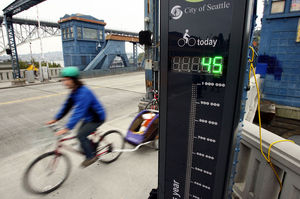
\includegraphics[width=1\textwidth]{figures/FremontBikeEcoCounter.jpg} 
  \caption{EcoCounter on the Fremont Bridge}
  \label{fig:ecoCounter}
\end{figure*}

The bike count data used in this study cover a period of three years spanning from October 31, 2012 to October 30, 2015. The continuous bike count data is aggregated into daily counts. Note that in the literature, there is also studies on bike count modeling using hourly bike count. However, the daily bike counts are favored in this study because: 1) it carries less autocorrelation than the hourly data; 2) it's intuitive and simple to interprate, 3) we believe for bicyclists commuting to work, they make the decision of riding based on the daily weather, as opposed to the recreational riders is more likely to make deicions on a hourly basis. 

\subsection{Weather Data}
Weather data are collected by a variety of sources and are aggregated by Forecast.io. These data are available through the company's web services API \cite{The-Dark-Sky-Company:aa}. Historical daily summaries are available for a range of weather variables including several specifically important to our model such as precipitation, daily minimum and maximum temperatures, sunrise, and sunset, etc.

We downloaded and processed these data programmatically using the R programming language along with several add-on packages \cite{Grolemund:2011aa,Wickham:2011aa,Couture-Beil:2014aa,Lang:2014aa,R-Core-Team:2014aa}. Bicycle counts were aggregated by day, and then joined to weather data by date. 

\subsection{Temporal Data}
In addition to the variables collected from the above-mentioned two sources, we were also interested in controlling for holidays and whether or not the nearby University of Washington was in session. These data were collected and coded manually from the National Holiday calendar as well as the University of Washington's historic academic calendar.


\section{Ordinary Least Squares Regression}
The ordinary least squares (OLS) regression is one of the most widely used techniques in Statistics to estimate the unknown parameters. The goal is to minimize the differences between the observed responses and the predicted response given by the linear approximation of the data. The basic linear regression model assumes the following structure:
\begin{equation}
Y = \alpha + \beta X + \epsilon, \label{eqn:olsregression}
\end{equation}
where $Y$ is the response variable (or observations, dependent variable), and $X$ is the predictors (or regressors, independent variables), $\alpha$ and $\beta$ are the unknown parameters to estimated, and $\epsilon$ is the unobserved scalar random variables (errors) which accounts for the discrepancy between the actual observed responses $Y$ and the predicted responses $\alpha + \beta X$.  

The OLS techinque offers a mathematically convinient tool to estimate the linear regression model parameters $\alpha$ and $\beta$. There are many available software packages to provide solutions to the linear problem~\eqref{eqn:olsregression}, i.e., the \texttt{lm} function in \texttt{R}. However, to properly apply the OLS estimators, certain assumptions need to be checked beforehand, such as: 1) No linear dependence (no multicolinear), 2) Strict Exogeneity ($E[\epsilon|X]=0$), 3) Homoscedasticity ($E[\epsilon^2|X]=\sigma^2$), and 4) Normality (the error term has a normal distribution). For more details on OLS regression models, readers are referred to~\cite{}.

The goodness-of-fit of the considered model is often evaluated with the $R^2$ (R squared, or the coefficient of determination) and adjusted $R^2$. The $R^2$ measures the percentage of the response variable variation that is explained by a linear model, or equivalently
\begin{equation}
R^2 = 1- \frac{\text{Residual Sum of Squares}}{\text{Total Sum of Squares}}.\label{eqn:R2}
\end{equation}
The adjusted $R^2$ adds a correction for the number of estimated parameters to guard against overfitting. Other important goodness-of-fit criterions that are used in this study are the Akaike Information Criterion (AIC) and the Bayesian Information Criterion (BIC). Details on the latter two can be found in~\cite{}.

\section{Generalized Linear Model (GLM)}

\section{Generalized Additive Mixture (GAM) Model}
\label{sec:gamintro}
The generalized additive model (GAM) is a generalized linear model in which the linear response variable depends on unknown smooth functions of the independent variables~\cite{Wiki}. The goal is to provide characterization about these smooth functions. GAM was first proposed in~\cite{Hastie86}	 to blend the properties of generalized linear models with additive models. 

Following a similar approach with the GLMs, an exponential family distribution (could also be Poisson, normal, negative binomial, etc) is specified for response $Y$ along with a link function $g$ relating the expected value of $Y$ to the predictors $X_i$ such as
\begin{equation*}
g(E[Y]) = \beta_0 + s_1(X_1) + s_2(X_2) + \hdots + f_m(X_m)
\end{equation*}
The function $f_i(X_i)$ may be specified parametric functions (e.g., polynomial) or may be specified non-parametrically, or semi-parametrically, simply as 'smooth functions', to be estimated by non-parametric means. The nonparametric GAM provides a very general modular estimation method capable of using a wide variety of smoothing methods to estimate the $f(X)$. The advantage of non-parametric models is that they are easy and efficient to fit, while the disadvantage is the inability to control the complexity of the model (degree of smoothness of $f(X)$), which often gives rise to problems with interpretation. Overall, a well calibrated GAM is likely to perform better than nearly any other model type, if the dataset is large enough and its behavior is complex enough. However, it could also have problems of overfitting as the number of smoothing parameters increases. 

In this thesis, we use the GAM model to explore the potential relationship between the dependent variable bike counts and weather factors (i.e., temperature and precipitation). It is noticed in other studies~\cite{} that the temperature has a positive effect on ridership when its below, and a negative impact when higher than. Also, the temperature squared is often used in the literature~\cite{} to account for the nonlinearity without good explanation. The GAM provides a good starting point to investigate such nonlinear relationship since it explicitly models the dependent variable on a smooth function of the independent variable. Consequently, resulting non-parametric smooth function provides valuable insight on how to include nonlinear terms in the recommended model. In this thesis, the \texttt{gam} in \texttt{R} is used to fit generalized additive models, specified by giving a symbolic description of the additive predictor. \texttt{gam} uses the backfitting algorithm~\cite{} to combine different smoothing or fitting methods. The default built-in nonparametric smooth splines are used to fit the model. 

\section{Autoregressive Integrated Moving Average (ARIMA) Model}
\label{arimaintro}

The ARIMA method usually consists of three major components: differencing, autoregressive model and the moving average mode. The differencing step is used to convert the time series to be stationary, which means there is no predictable patterns in the time series in the long run. The Autocorrelation Function (ACF) plot is also useful to identify non-stationary series. The ACF plot depicts the autocorrelation between the $Y_t$ and its lagged values $Y_{t-k}$ for different values of k. By definition of stationarity, for a stationary time series, its ACF will drop to zero relatively quickly, while the ACF of non-stationary data decreases slowly. Other two popular statistical stationarity tests are the Augmented Dickey-Fuller (ADF) test and the Kwiatkowski-Phillips-Schmidt-Shin (KPSS) test, both available in \texttt{R}.

In a pure autoregressive model, the dependent variable $Y$ consists only of lagged values of itself. In other words, we forecast $Y$ using a linear combination of past values of the variable. A moving average model, however, uses the past forecast errors in a regression-like model. It means that each value of $Y_t$ can be thought of as a weighted moving average of the past few forecast errors. 

By combining the above three components: differencing, autoregressive model and the moving average model, we have the non-seasonal ARIMA model. The mathematical expression for the full model is as follows:
\begin{equation}
y'_t = c + \phi_1 y'_{t-1} + \phi_2 y'_{t-2} + \hdots + \phi_p y'_{t-p} + \theta_1 e_{t-1} + \theta_2 e_{t-2} + \hdots + \theta_q e_{t-q} + e_t, \label{eqn:ARIMA}
\end{equation}
where $y'_t$ is the first-differenced time series, and $e_t$ is the white noise error. Equation~\eqref{eqn:ARIMA} is referred to as the ARIMA($p,d,q$) model, where $p$, $d$, $q$ is the order for autoregressive, differencing and moving average model, respectively. To choose an appropriate order ($p,d,q$) for ARIMA, one can use a combination approach of automated procedure \texttt{auto.arima} in \texttt{R} and direct observations of ACF and PACF plots. Recall that the PACF measures the relationship between $y_t$ and $y_{t-k}$ after removing the effects of other time lags in between: $1, 2, 3, \hdots, k-1$. The best model is chosen according to the smallest AICc. Note that it is also not common to have an ARIMA model of order more than 3.

Last but not least, it is also possible to include exogenous regressors in the ARIMA model. The mathematical expression for ARIMA with regressors is as follows:
\[Y_t = \beta_t X_t + n_t\]
where $X_t$ is the vector of regressors and $n_t$ is the an ARIMA($p,d,q$) model. In other words, the ARIMA($p,d,q$) model is fitted to the errors of the regression of $y$ on $X$ (i.e., the series $y_t - \beta_t X_t$). More details on ARIMA and its implementation could be found in~\cite{Hall11}.


% ========== Chapter 4
 
\chapter{Analysis and Results}

This chapter discusses the process and result of analyzing different regressors in relation to cycling and how they are used to predict future cycling. It starts with a systematic study on selecting important explanatory variables as well as the right regression model to fit bike count data. Then it discusses how these explanatory variables influence cycling. The impact of different weather variables, seasonal factors as well as interaction terms are thoroughly investigated and interpreted. Moreover, a Generalized  Additive Mixture model is utilized to explicitly capture the nonlinear relationship between bike counts and weather conditions. All results are illustrated with the intuitive simulation visually. Lastly, a predicative model with certain predictors and Autoregressive Integrated Moving Average (ARIMA) error terms is proposed to predict cycling count. It will account for possible autocorrelation in time series and its predicative performance is proven through cross validation.


\section{Exploratory Data Analysis and Variable Selection}
\label{sec:eda}

The initial modeling data is assembled as described in Section~\ref{sec:data}, with daily bike count data sourced from City of Seattle, daily weather variables retrieved from \texttt{Forecast.io}, and seasonal factors collected from public information (i.e., national holiday from~\cite{holiday} and UW in session status from~\cite{uwcalendar}). This original data consists of a rich pool of 34 variables, out of which 26 are related to weather variables, 7 are related with seasonal factors and 1 dependent variable being the daily bike counts. Figure~\ref{fig:descriptionbc} provides a visual summary of the bike counts data. Some apparent outliers are visible at the rightmost portion of the histgram. The two highest counts occurred the Monday and Tuesday preceding the beginning of National Bike to Work Month. And the third highest count occurred on National Bike to Work Day.

\begin{figure*}
\begin{tabular}{ll}
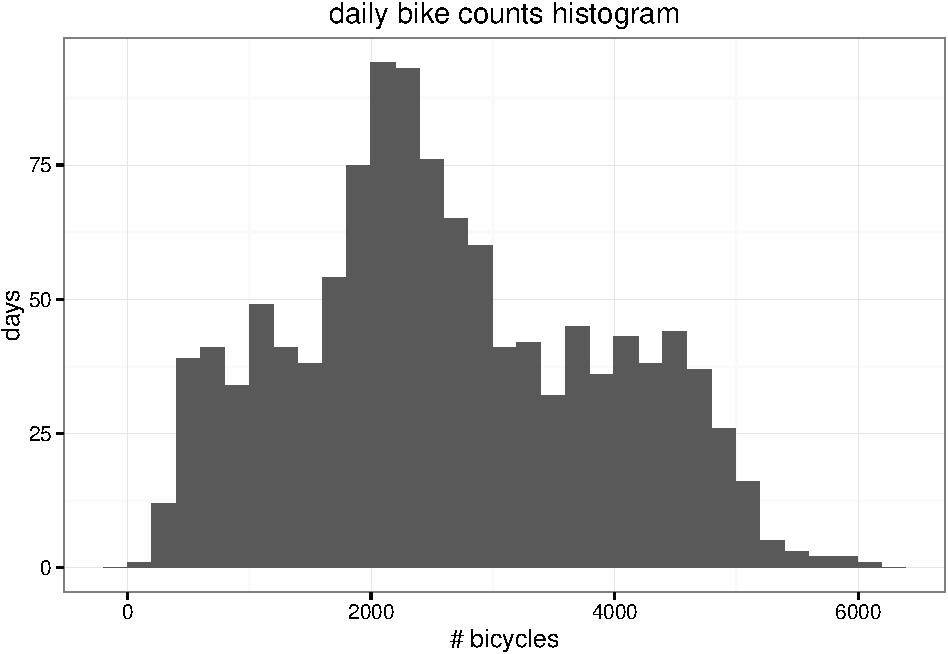
\includegraphics[width=0.45\textwidth]{figures/daily_hist}
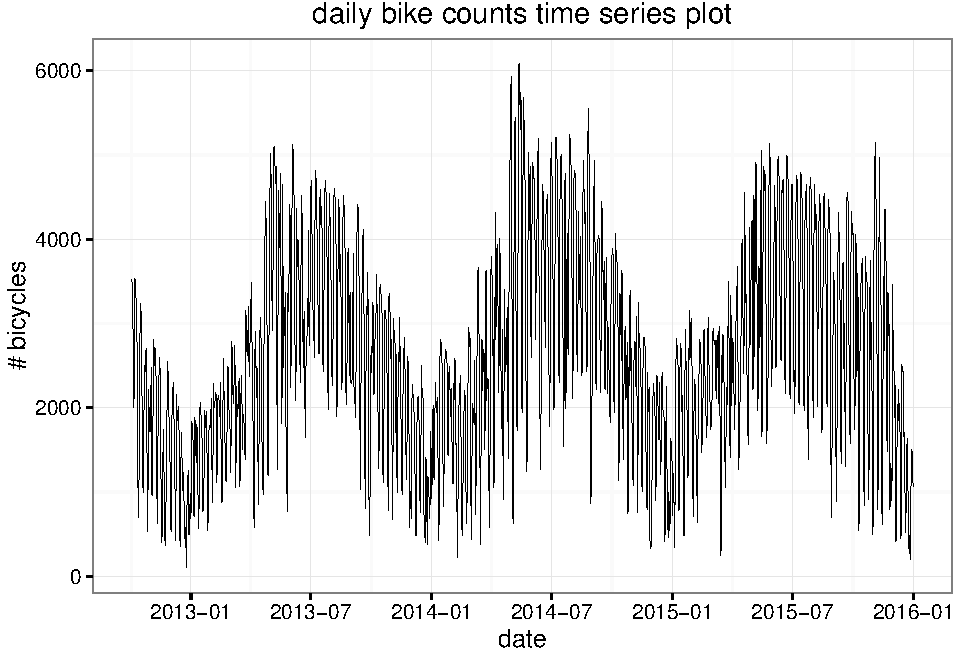
\includegraphics[width=0.45\textwidth]{figures/daily_tscount_plot}\\
\end{tabular}
\caption{Descriptive visualization of bicycle counts dataset: (a) Frequency of observed counts; (b) Timeseries of counts.}
\label{fig:descriptionbc}
\end{figure*}

Out of the set of independent variables, we selected a subset of variables that we felt best reflected our research questions. To do so, we adopt a systematic approach to extract the relevant variables and the proper format if multiple choices are available.

\subsection{Weather variables selection}
Weather variables have a huge impact on daily bike counts because cyclists are fully exposed to outdoor conditions. Therefore, one of our major goals is to identify relevant weather variables that provide the highest explanatory power for the variation in bike counts. Literature has unanimously agreed that temperature and precipitation are the two main weather determinants for bike ridership~\cite{Nosal:2014aa,Tin:2012aa}. In general, cycle counts increases with temperature. However, with daily-aggregated weather information, decision needs to be made regarding what form of the temperature variable should be used in the model, e.g., the daily maximum temperature or the mean temperature. In the literature, arguments have been made for each case. For example, in the work by Tin Tin et. al~\cite{Tin:2012aa}, the maximum temperature is used because people are most sensitive to the extreme, while in Thomas et. al~\cite{Thomas09}, the mean temperature is used because the authors believe that many cyclists make their trips in the morning, during which the temperature lies closer to the mean. In this study, daily maximum temperature \texttt{MaxTemp}, measured in Fahrenheit, was chosen to represent temperature in part to retain simplicity in the model, in part because there is relatively little daily temperature variation in Seattle due to the moderating effect of large water bodies, and in part because maximum temperature better reflects the conditions during daylight hours when most bicycle trips would occur. This simplification may not be warranted for other locations that experience greater temperature variation than Seattle. 
% The squared daily maximum temperature is also included to account for potential nonlinear relationship. Such nonlinear relationship is 

Precipitation, or rainfall, also have a significant impact on the cycling counts. However, similar to temperature, there are multiple choices of the precipitation variable in the original dataset that could be used in the model, such as the precipitation amount~\cite{Ahmed12}, duration of the precipitation~\cite{Thomas09}, rain presence~\cite{Miranda-Moreno:2011aa}, etc. In this study, the precipitation probability \texttt{PrecipProb}, which measures the probability of precipitation for the day, was chosen rather than other alternatives based on the assumption that bicyclists usually make travel decisions based on the likelihood of raining \emph{ahead} of the day, while variables such as maximum precipitation or precipitation duration in the \texttt{Forecast.io} report only represent the fact \emph{after} the rainfall have occurred. As in the case of temperature, this simplification would be less justifiable in locations that experience greater daily variation in precipitation or in locations that have a predictable pattern of precipitation during certain hours.

Besides temperature and precipitation, other weather variables have been identified in the literature to have different levels of influence on cycle counts. In the work of Moreno and Nosal~\cite{Miranda-Moreno:2011aa}, humidity is found to have a negative relationship with cycling. The factor of wind speed is shown to be significant in~\cite{Thomas12}, while in the tests by~\cite{Miranda-Moreno:2011aa} wind speed had no impact on the results. Other variables that have been examined include sunshine~\cite{Thomas12}, cloud coverage~\cite{Hanson77}, dew point~\cite{Schade14,Nosal:2014aa} and visibility~\cite{Thomas09}. Considering their relatively insignificant impact on cyclist counts and for the purpose of simplification,\texttt{cloudCover}, \texttt{dewPoint}, \texttt{humidity}, \texttt{moonPhase}, \texttt{visibility}, \texttt{windBearing}, \texttt{windSpeed} are excluded in further analysis. \texttt{sunriseTime} and \texttt{sunsetTime} variables are used to generate the \texttt{daylight} variable, which will be used as a factor for seasonality.

\begin{figure*}
  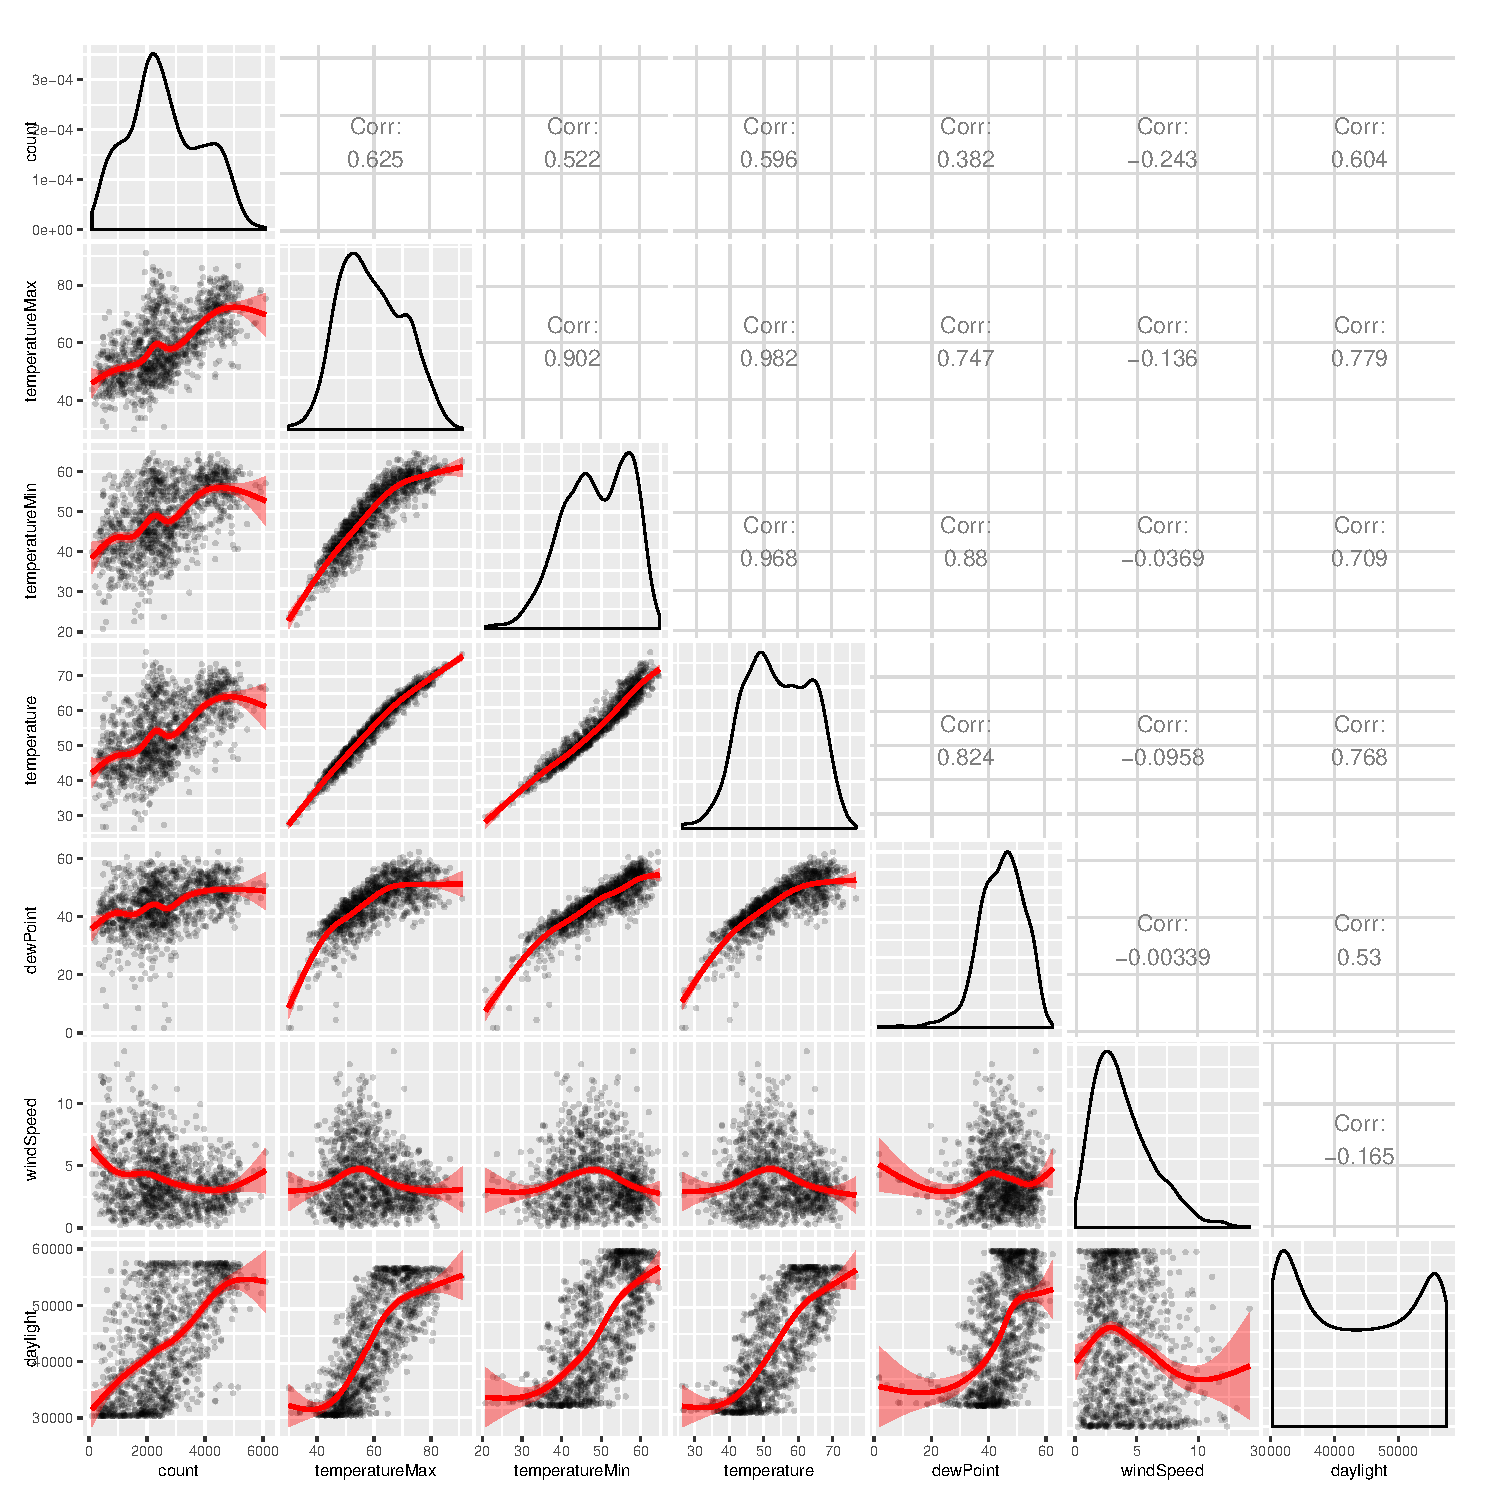
\includegraphics[width=1\textwidth]{figures/matrix2}
  \caption{Scatter plot Matrix of covariates in the Group of Temperature and the Response}
  \label{fig:temp_corr}
\end{figure*}

To support our choice on the selected weather variables \texttt{MaxTemp} and \texttt{PrecipProb}, the correlation scatter matrix is depicted as in Figure~\ref{fig:temp_corr}. It is shown that all temperature related variables have similar correlations with bike counts, and very high correlation with each other (more than 0.9). To avoid collinearity it is reasonable to keep only \texttt{MaxTemp} because it has the highest correlation with bike counts.  

\begin{figure*}
   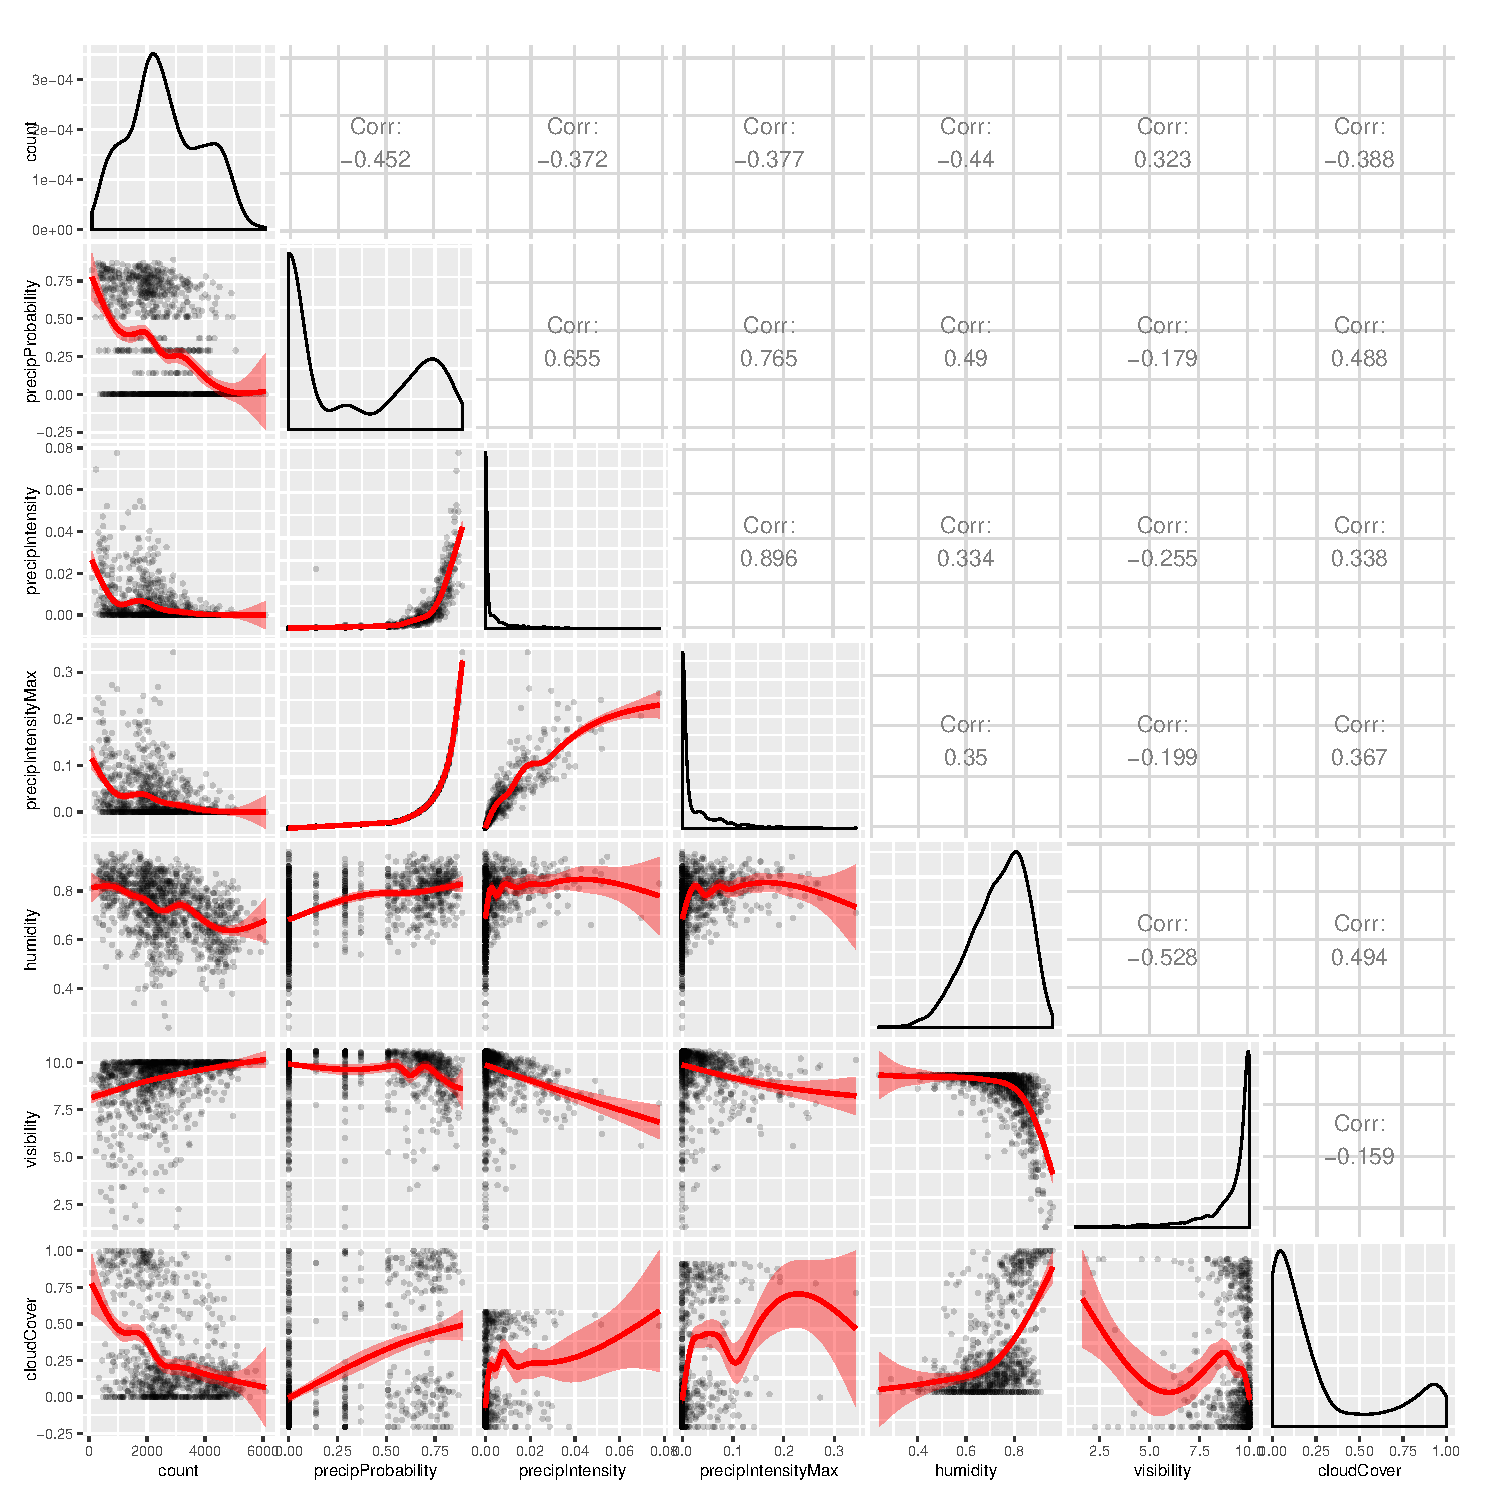
\includegraphics[width=1\textwidth]{figures/matrix1}
  \caption{Scatterplot Matrix of covariates in the Group of Precipitation and the Response}
  \label{fig:precip_corr}
\end{figure*}

Similarly, in the scatter matrix Figure~\ref{fig:precip_corr}, it is noted that correlation between the probability of precipitation and the response count is -0.452, stronger than the rest of precipitation-related variables. At the same time, there exist high correlations between 'precipProbability' and other variables such as 'precipIntensityMax', 'precipIntensity', and 'humidity'. To avoid collinearity we decided to keep \texttt{PrecipProb} in our model.

The last weather variable we include for further testing is the categorical variable \texttt{Weather}, which represents the general weather classification, such as 'clear-day','cloudy','foggy','rainy','windy', etc. The rationale behind this is that bicyclists will simply make their travel decision based on the general weather description, instead of detailed numeric information such as the exact temperature degree or the precise rainfall inches. The \texttt{Weather} variable serves as the best summary of weather conditions and could potentially reduce the model complexity.

\subsection{Seasonal factors}
Seasonal factors are also found to have significant impact on bike counts in the literature. Such impact may be caused by weather, holidays, working schedules and school calendars, etc.

Daylight hours \texttt{Daylight} (defined as sunset time $-$ sunrise time) was selected to represent seasonality. One possible justification for choosing daylight hours over the calendar-based categorization of season is in part because Seattle’s Pacific Maritime Climate differs substantially from traditional notions of four seasons. Daylight hours also is measured as a continuous value at a finer temporal resolution of one day. Finally, daylight hours adjusts according to latitude, which may make this model estimation procedure and specification more transferable to other sites in the future, perhaps by interacting latitude with daylight hours. For the sake of comparison, the traditional \texttt{Season} variable is also included, which can takes Boolean values in 'Spring', 'Summer', 'Autumn' and 'Winter' as dummy variable.

University of Washington in-session status \texttt{UW} was selected to represent seasonality as well. We deemed the University of Washington variable important in part because of the Fremont Bridge's proximity and connection via the Burke Gilman Trail to the University of Washington. We also felt that this variable was a suitable proxy for the 'school season', which more broadly captures whether or not other local schools are in session. The academic calendars of the various local schools do not align perfectly, however they still overlap substantially with the University of Washington, which is itself the largest educational institution in the region.

Inclusion of the holiday variable \texttt{holiday} was an attempt to account for some low outlier counts. Upon inspection of the dataset, Christmas and Thanksgiving in particular had very low counts of bicycles relative to the days preceding and following. Relatedly, but not accounted for by any variable in our model, are some of the high outlier counts. Upon inspection, some of the highest counts were observed on National Bike to Work Day and on the day of the Fremont Solstice Parade, which typically draws large numbers of bicyclists as participants and spectators. The omission of such a variable is justified based on the few occurrences of high outlier counts, and our desire for this model to only include variables that could be collected or straightforwardly adapted to other locations.

Day of the week \texttt{dow} was added due to its presence in the literature, as well as an apparent weekly pattern revealed visually by zooming into the time series plot. These data were coded as a set of Boolean dummy variables, excluding Friday as the reference category. In addition, the weekend or not flag \texttt{Weekend} is included since we are interested in understanding the traveling behaviour of commuting bicyclists. It is expected to have big variation in bike counts between weekends and weekdays but not so much between individual day of the week. 


\begin{figure*}
\vspace{-40pt}
\begin{tabular}{ll}
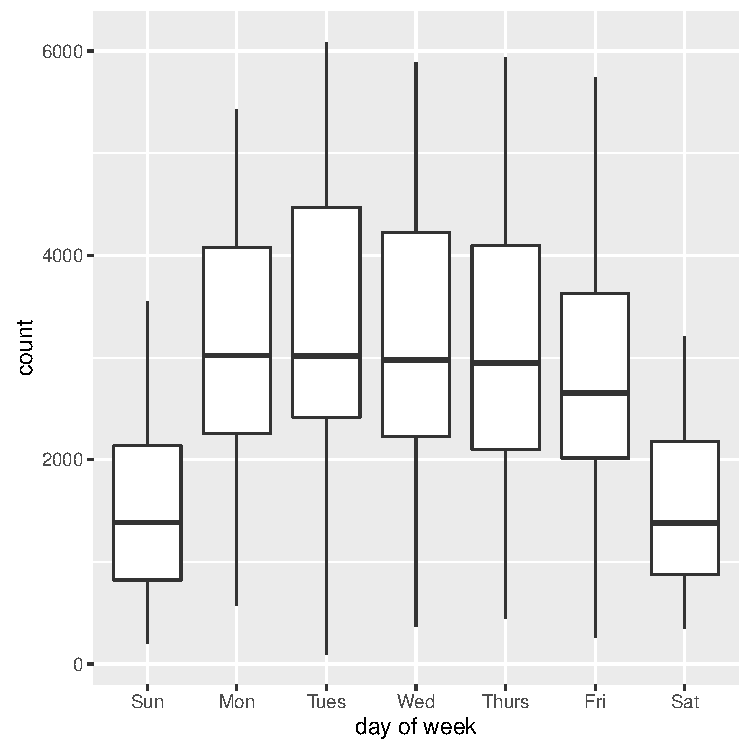
\includegraphics[width=0.45\textwidth]{figures/dow_cat}
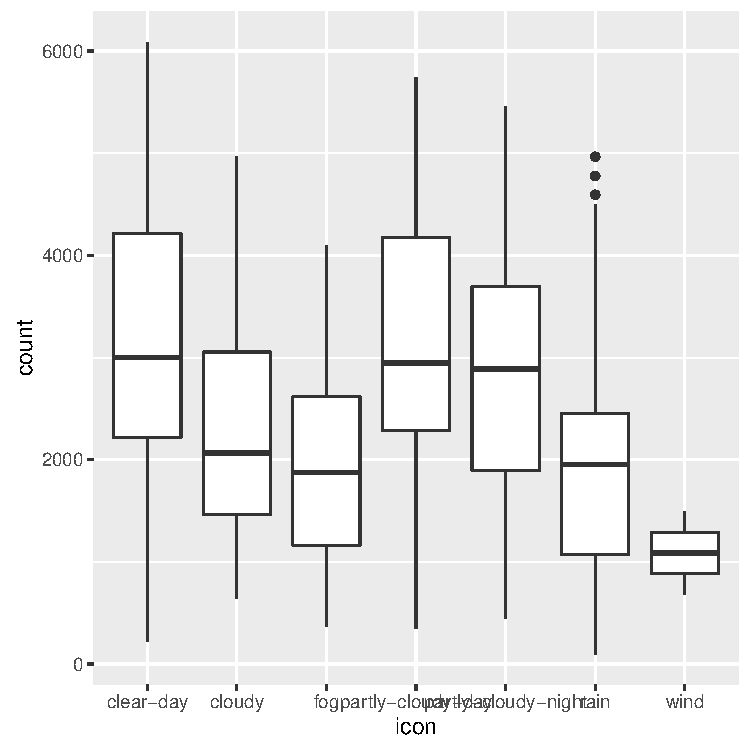
\includegraphics[width=0.45\textwidth]{figures/icon_cat}\\
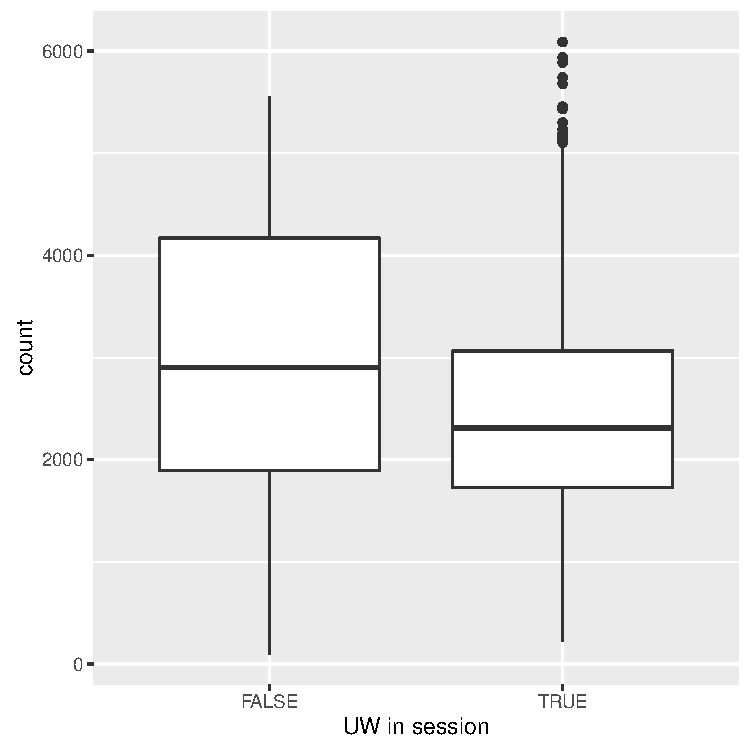
\includegraphics[width=0.45\textwidth]{figures/uw_cat}
\includegraphics[width=0.45\textwidth]{figures/wknd_cat}\\
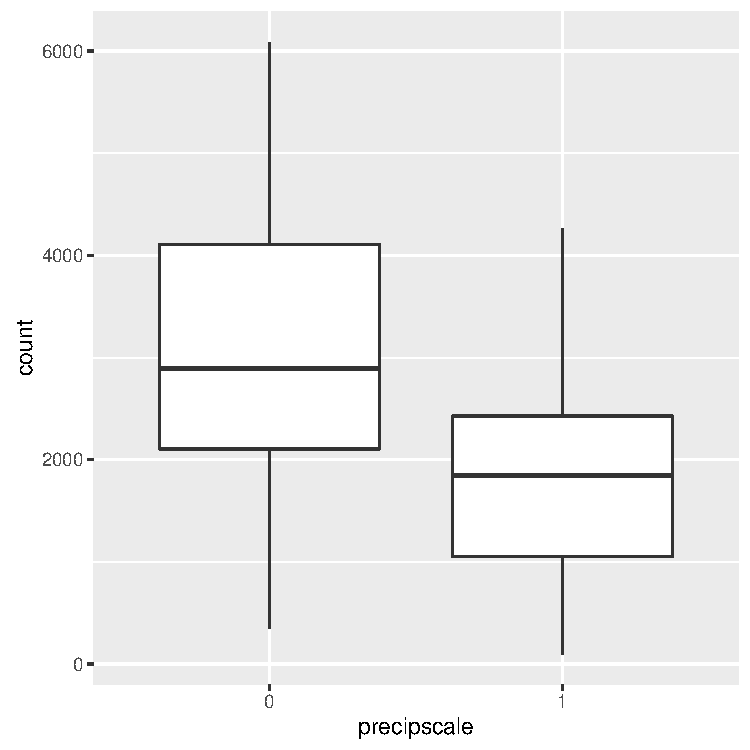
\includegraphics[width=0.45\textwidth]{figures/scale_cat}
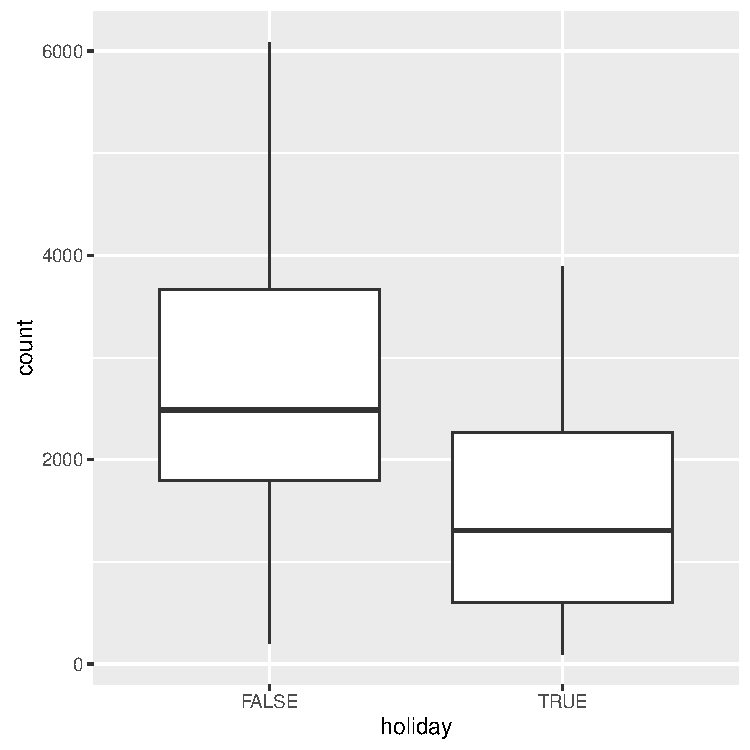
\includegraphics[width=0.45\textwidth]{figures/holiday_cat}\\
\end{tabular}
\vspace{-10pt}
\caption{Boxplots of ``dow", ``weather, ``uw'', ``wknd", ``prepscale", and ``holiday"  versus ``count''}
\label{fig:cat_bxplot}
\end{figure*}

The final variable, the time index \texttt{T}, was included so that we could test for a linear trend in bicycling volumes. We created this variable by sequentially numbering (1--1157) the observed counts by day during the study period.

Box plots for categorical variables against the response daily bike count is depicted in Figure~\ref{fig:cat_bxplot}. Visually, we are able to observe the difference in their means, suggesting these variables have the explanatory power to explain variation in the bike data. However, formal statistical tests need to conducted to confirm their significance, which would be a subject of Section~\ref{sec:intrepofresult}.

\subsection{Summary of this section}

Combining results from the above analysis, a subset of explanatory variables is extracted from the original dataset. Their names and descriptions are summarized in Table~\ref{tb:variables}. Note that this list of variables are \emph{not} the final list of variables used in the model and will be used in the final model at the same time. It just represents the group of variables that we will be testing with in the following sections. 

\begin{table}
\begin{center}
\caption{Explanatory variables}
\vspace{10pt}
\begin{tabular}{l l} 
 \hline
Variable & Description \\
\hline
\texttt{Count*} & Number of bicycles per day \\
\texttt{MaxTemp} & The maximum temperature for the day \\
\texttt{PrecipProb} & Probability of precipitation for a given day \\
\texttt{Daylight} & Time from dawn to dusk in hour\\
\texttt{dow} & Day of the week dummy variable (from Sat. to Thursday.) \\
\texttt{Holiday} & The day was a holiday as recognized by UW (TRUE/FALSE) \\
\texttt{Weekend} & The day is a weekend (TRUE/FALSE) \\
\texttt{UW} & The University of Washington was in session (TRUE/FALSE) \\
\texttt{Season} & Season indicator spring, summer, autumn, and winter \\
\texttt{Weather} & General weather classification, such as ``clear-day'', ``cloudy'', ``foggy'', \\
 & ``rainy'', ``windy'', ``partly-cloudy-day'', ``partly-cloudy-night'' (7 levels)\\
\texttt{T}  & Time index (sequentially day) during study period \\
\hline
\label{tb:variables}
\end{tabular}
\end{center}
\end{table}



\section{Choices of Model}
\label{sec:choiceofmodel}

Since the daily bike count data is non-negative and discrete-valued, a natural model choice to fit the bike count data would be Poisson model~\cite{Niemeier:1996aa} or the negative binomial model~\cite{PeterWeiran16} if over-dispersion is observed in the data. Neverthesless, recall that in Figure~\ref{fig:descriptionbc} of Section~\ref{sec:eda}, the distribution of daily bike counts follows an approximate Gaussian distribution. Moreover, we have collected count data over a long period of time of data (3 years) and it could be treated as if it was continuous-valued. Therefore, both a Poisson model and OLS-based linear regression model are considered in this study.

\begin{table}
\begin{center}
\caption{Four Type of Model}
\vspace{10pt}
\begin{tabular}{l|l} 
 \hline
Method & Regression equation \\
\hline
Standard linear regression & $Y=\alpha+\beta X + \epsilon$ \\
Exponential model & $\log{Y} = \alpha + \beta X + \epsilon$ \\
Quadratic model & $\sqrt{Y} = \alpha + \beta X + \epsilon$ \\
Poisson model & $\log{E(Y|X)} = \alpha + \beta X $\\
\label{tbl:choiceofmodel}
\end{tabular}
\end{center}
\end{table}

In addition, certain model requirements need to be examined when choosing the right OLS regression models, i.e., homoscedasticity, normality assumption, etc. It can be shown that some of the key assumptions for regular linear regression model are indeed violated. Fortunately, one can apply certain type of nonlinear transformation to the dependent variable to eliminate skewness and other distributional features that complicate analysis. Common transformations include logarithm and square root.

To fix the idea, we first fix the explanatory variables $X$ to be \texttt{TempMax}, \texttt{Holiday}, \texttt{PrecipProb}, \texttt{Weekend}, and \texttt{Daylight}. The following choices of model are considered: standard linear regression, exponential model (with logarithm transformation), quadratic model (square root transformation) and the Poisson model. Their corresponding regression equations are described in Table~\ref{tbl:choiceofmodel} (Using the vector notation as in~\eqref{eqn:olsregression}).

Note that the Poisson model is also called the log-linear model. It assumes the response variable $Y$ follows a Poisson distribution, and assumes the logarithm of its expected value can be modeled by a linear combination of unknown parameters.

%Log-linked Gassuian (glmlog):
%\begin{equation}
%\log(E[\text{Count}_t]) = \beta_0 + \beta_1 \text{TempMaxSq}_t + \beta_2 \text{Holiday}_t + \beta_3 %\text{PrecpProb}_t + \beta_4 \text{Weekend}_t + \beta_5 \text{Daylight}_t,\label{eqref:glmlog_model}
%\end{equation}
%where $\log(\text{Count}_t)$ is assumed to follow a standard Gaussian distribution.
%\end{enumerate}

%Negative Binomial:
%\begin{equation}
%E[\text{Count}_t|X] = \beta_0 + \beta_1 \text{TempMaxSq}_t + \beta_2 \text{Holiday}_t + \beta_3 \text{PrecpProb}_t + \beta_4 \text{Weekend}_t + \beta_5 \text{Daylight}_t,\label{eqref:poisson_model}
%\end{equation}
%where $\text{Count}_t$ is assumed to follow a negative binomial distribution.

\begin{figure*}
   \includegraphics[width=1\textwidth]{figures/y_transform} 
  \caption{Model comparison for different $Y$ transformations}
  \label{fig:y_transform}
\end{figure*}


The following residual over fitted value plot are presented to evaluate different transformations. Based on comparison, we will choose the right model structure to estimate the mean.
\begin{enumerate}
\item \textbf{Residual vs. Fitted plot:} A plot of the residuals against the fitted values should show no pattern. If a pattern is observed, there may be 'heteroscedasticity' in the errors. That is, the variance of the residuals may not be constant. This indicates a transformation of the dependent variable may be required. It is shown in Figure~\ref{fig:y_transform} that the model with original bike count as dependent variable has a clear varying variance in its residual: the residual becomes larger when the bike counts to be predicted become larger. Among the four  models we tested, the quadratic model (square root transformation) results in the best residual plot, which remains constant for all fitted values. 
\item \textbf{Normal Q-Q plot:} The Normal Quantile-Quantile (Q-Q) plot represents an informal graphical test of the hypothesis that a data sequence is normally distributed. That is, if the points on a normal Q-Q plot are reasonably well approximated by a straight line, the Gaussian data hypothesis is plausible, while marked deviations from linearity provide evidence against this hypothesis~\cite{Pearson2011}. It is shown in Figure~\ref{fig:y_transform} that all models under consideration don't have a perfectly Normal distributed residuals, as is required by the linear regression models. For the quadratic model, the residual error has a slightly heavy tail on the right side. 
\item \textbf{Scale-Location plot:} It depicts the square root of the absolute values of the residuals against the fitted values, with a Lowess curve helpfully overlaid. The scale-location plot is often used to check if the data possesses homoscedasticity, which is required for the linear regression model. Ideally if the modeling data has homoscedasticity, the Lowess curve is expected to be flat, not sloped, and the square root of residuals should be approximately evenly distributed along the Lowess curve. Using this criterion, it is shown in Figure~\ref{fig:y_transform} that the quadratic model has the least heteroscedasticity because its Lowess curve is relatively flat and the residual didn't show a obvious pattern.
\item \textbf{Residual vs. Leverage plot:} This plot depicts the standardized residuals against the leverage for each point in the data series. The Cook's Distance is also shown in the plot. This plot is mainly used to identify extreme points and possible outliers in the data series that could shift the regression line significantly. The further out the point is on the $X$ or $Y$ axis, the more leverage or standardized residual the point in data set has. More details on the Residual vs. Leverage plot could be found in~\cite{gung13}. From Figure~\ref{fig:y_transform} it can be seen that there are a few points in the data set that have large leverage on the regression lines (indicated by points at the far right side of the plot). The Poisson model has relatively larger residuals with quite a few points with big Cook's distance. This indicate the Poisson model might not be a good fit. For each model, there is one point has big positive error (1107). This outlier point corresponds to the 'City Bike to Work Day', on which there are more than six thousand bikes passing the Fremont Bridge on the same day. This suggests proper data cleaning is required (i.e., removing outliers) to best capture the relationship between utilitarian bike ridership and weather/seasonal factors. 
\end{enumerate}

\begin{table}
\caption{Goodness-of-fit of models} 
  \label{tbl:ytransform} 
\small
\begin{tabular}{ c | c | c | c | c } 
\hline 
  Model Name & Standard Linear Model & Exponential Model & Quadratic Model & Poisson Model \\ 
\hline
  $R^2$  & 0.84 & 0.82 & 0.86 & 0.85 \\ 
  mse  & 501.46 & 541.14 & 477.48 & 495.28 \\ 
\hline 
\end{tabular} 
\end{table} 

From the above analysis, the quadratic model with square root transformation of $Y$ appears to best stabilize the varying variance in the original data set. To better justify this, we also applied the Box-Cox test~\cite{boxcox64} to find out the optimal transformation parameter $\lambda$ such that the transformed dependent variable (defined as $T(Y) = (Y^{\lambda}-1)/\lambda$) follows an approximately normal distribution. As is shown in~Figure~\ref{fig:boxcox}, the optimal transformation parameter lies between 0 and 1, and is approximately 1/2, which confirms our previous conjecture.

Furthermore, we compare the goodness-of-fit of four type of models. The results are summarized in Table~\ref{tbl:ytransform}, where $R^2$ and mean squared error are provided. As can been see in Table~\ref{tbl:ytransform}, the quadratic model has the highest $R^2$ and smallest mean squared error, suggesting a better fit than the rest three.

In summary, the quadratic model can best accommodate the original data set: after applying the square root transformation to the dependent variable, the resulting model residuals have an approximate constant variance; error terms follow an approximate Gaussian distribution; the homoscedasticity assumption is satisfied. Therefore, the exponential regression model with square root transformation will be adopted in the following analysis. 

\begin{figure*}
\centering
   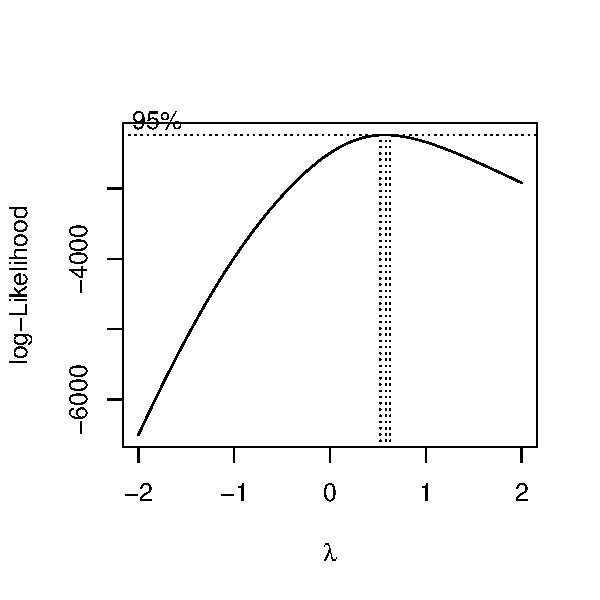
\includegraphics[width=0.5\textwidth]{figures/boxcox} 
  \caption{Box-Cox test }
  \label{fig:boxcox}
\end{figure*}

\section{Model Result and Discussion}
\label{sec:intrepofresult}

In this section, a detailed study on the impact of weather and seasonal variables on bike counts is provided. How different variables are related to bike count are discussed and interpreted in different models. A base model is developed to capture the major interested regressors while 6 additional models are used to address other interests such as non-linearity, discontinuity and interaction relationship. A summary of all model specifications considered appears in Table~\ref{tbl:model_spec}. Before developing different model specification, a Generalized Additive Mixture Model (GAM) is used to test the nonlinear relationship between bike counts with temperature and precipitation. So model0 and model1 are develop the address nonlinearity. Model2, model3 and model4 are including variables that represent measurements of weather and seasonality on different scale (from continuous to categorical or to discrete characteristics). Model5 is testing interaction relationship between weather and season. And Model6 is quantifying the increase of cycling over time while controlling all the weather and seasonal factors. Model results are intrepreated using counterfactual simulations that visually showing the relationship. 

\begin{table}
 %\centering 
\caption{Model Specification} 
  \label{tbl:model_spec} 
\small
\begin{tabular}{ c | l } 
\hline 
  Name & Model Specification with Major Interest \\ 
\hline
  Model 0 & Base model : Include Non-linearity of \texttt{TempMax}\\ &
  \sqrt{count} $\sim$ \textbf{TempMax}^2  + TempMax + holiday + PrecipProb + Weekend+ Daylight + UW  \\ 
  Model 1 & Explore Non-linearity of \texttt{PrecipProb} \\ &
 \sqrt{count} $\sim$ TempMax^2  + TempMax + holiday + \textbf{PrecipProb + ppp} + Weekend+ Daylight + UW\\ 
  Model 2 & Explore the impact of different weather type :  \texttt{Weather}\\ &
  \sqrt{count} $\sim$ TempMax^2  + TempMax + holiday + PrecipProb + Weekend+ Daylight + UW+ \textbf{Weather}\\ 
  Model 3 & Explore the impact of different season :  \texttt{Season}\\ &
  \sqrt{count} $\sim$ TempMax^2  + TempMax + holiday + PrecipProb + Weekend+ UW + \textbf{Season}\\
  Model 4 & Explore Day of Week :  \texttt{dow}\\ &
  \sqrt{count} $\sim$ TempMax^2  + TempMax + holiday + PrecipProb + Daylight + UW + \textbf{dow} \\
  Model 5 & Explore the interaction betweeb \texttt{PrecipProb} and \texttt{Weekend}\\ &
  \sqrt{count} $\sim$ TempMax^2  + TempMax + holiday + \textbf{PrecipProb}*\textbf{Weekend}+ Daylight + UW\\
  Model 6 & Quantify trend by time index variable \texttt{T}\\ &
  \sqrt{count} $\sim$ TempMax^2  + TempMax + holiday + PrecipProb + Weekend+ Daylight + UW +\textbf{T}\\
\hline 
\end{tabular} 
\end{table} 


\subsection{Weather Impact}

It has been noticed in the literature that the temperature and precipitation have a nonlinear impact on bike ridership~\cite{Richardson00,Rose07}. In order to explicitly model nonlinearity, a generalized additive mixture (GAM) model is fitted to serve this purpose. The GAM methodology is described in Section~\ref{sec:gamintro}. Consider a GAM model of the following form:
\begin{equation}
\sqrt{E[\text{Count}_t]} = \beta_0 + \beta_1 s_1(\text{TempMax}_t) + \beta_2 \text{Holiday}_t + \beta_3 s_2(\text{PrecipProb}_t) + \beta_4 \text{Weekend}_t + \beta_5 \text{Daylight}_t. \label{eqref:gamodel}
\end{equation}
where $s_1$ and $s_2$ are two nonlinear smooth functions of \texttt{TempMax} and \texttt{PrecipProb}, respectively. A square root link function is used to connect the expected bike counts with the independent variables, as suggested in Section~\ref{sec:choiceofmodel}. The \texttt{gam} function of \texttt{mgcv} package in \texttt{R} is used to fit the model. By default, $s_1$ and $s_2$ will take the form of the built-in nonparametric smooth splines. The smoothing parameter is chosen automatically using cross-validation.

%\begin{figure}
%\centering
%\vspace{-1cm}
%   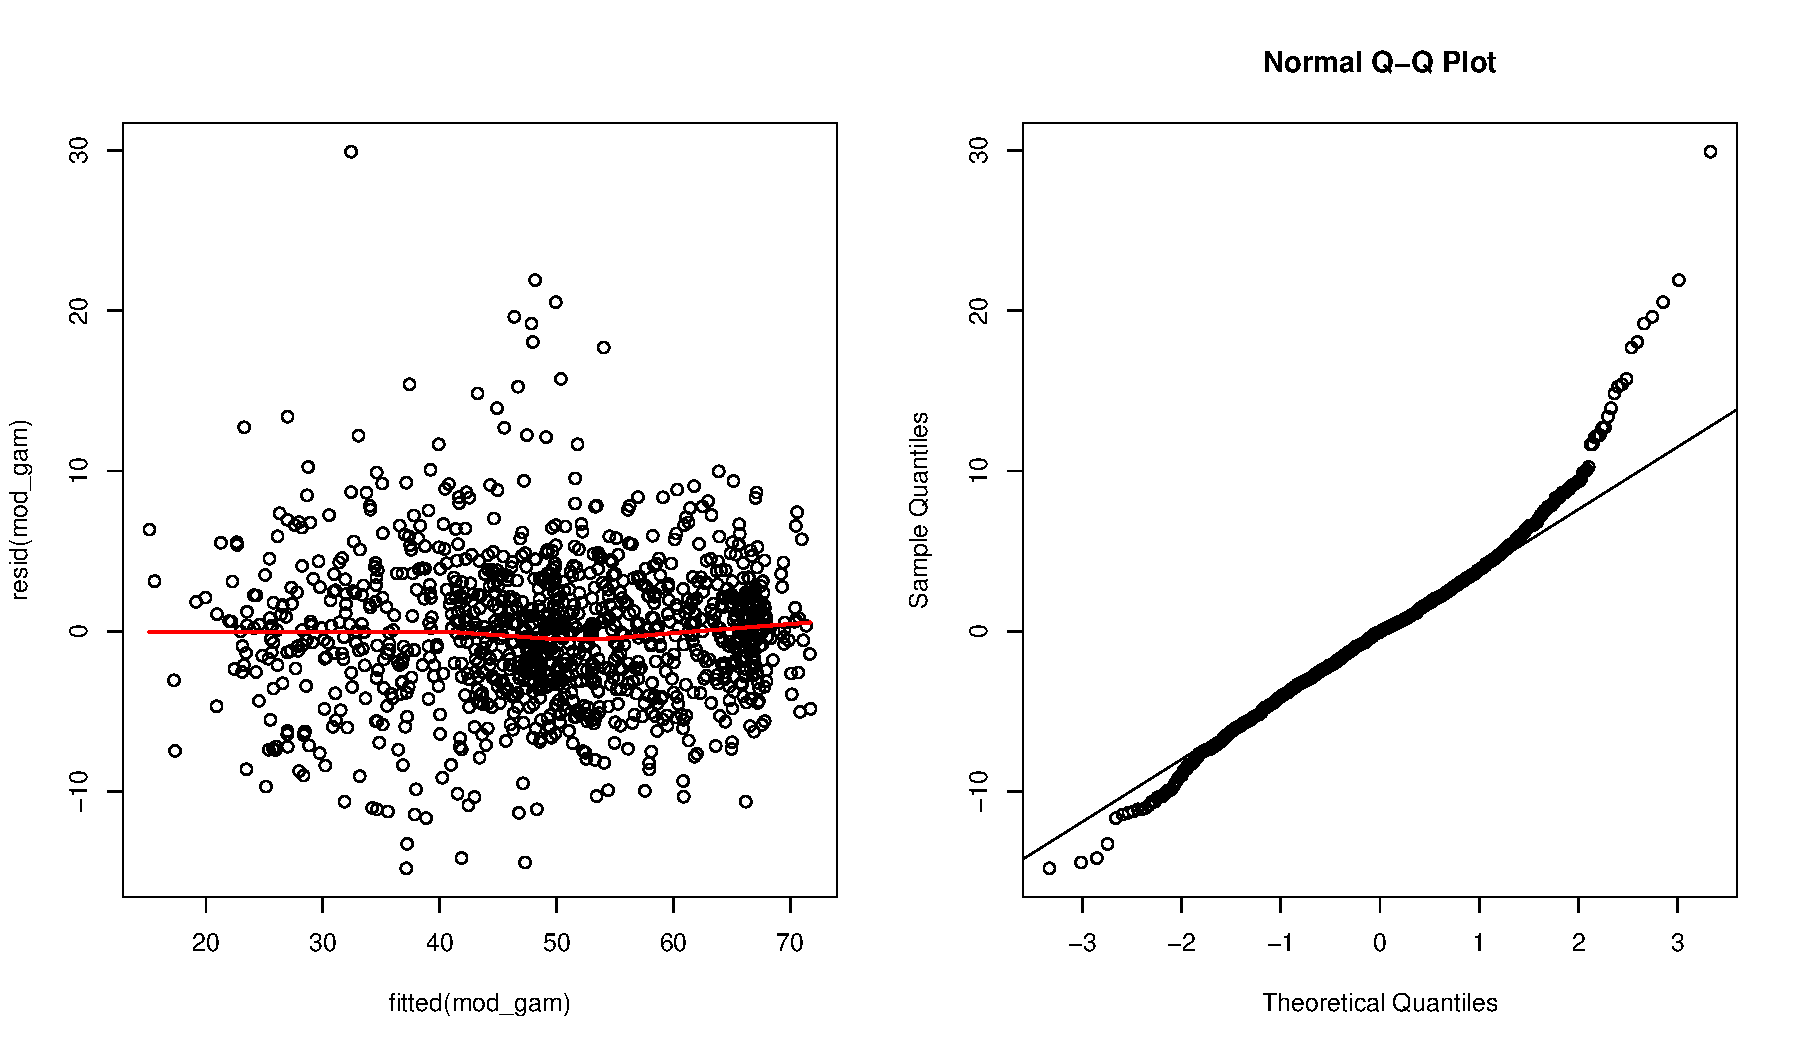
\includegraphics[width=1\textwidth]{figures/gam_resid} 
%  \caption{Residual vs. fitted plot and qq-plot for GAM fit.}
%  \label{fig:smooth_resid}
%\vspace{-1cm}
%\end{figure}

%The fitted GAM model is summarized in Table~\ref{gamtable}. \textbf{Add one paragraph on the GAM model summary}. As seen in Figure~\ref{fig:smooth_resid}, there is no discernable pattern in the Residual vs. Fitted value plot. Furthermore, the Normal Q-Q plot suggest that the residual follows an approximately Gaussian distribution. 

\begin{figure}
\centering
   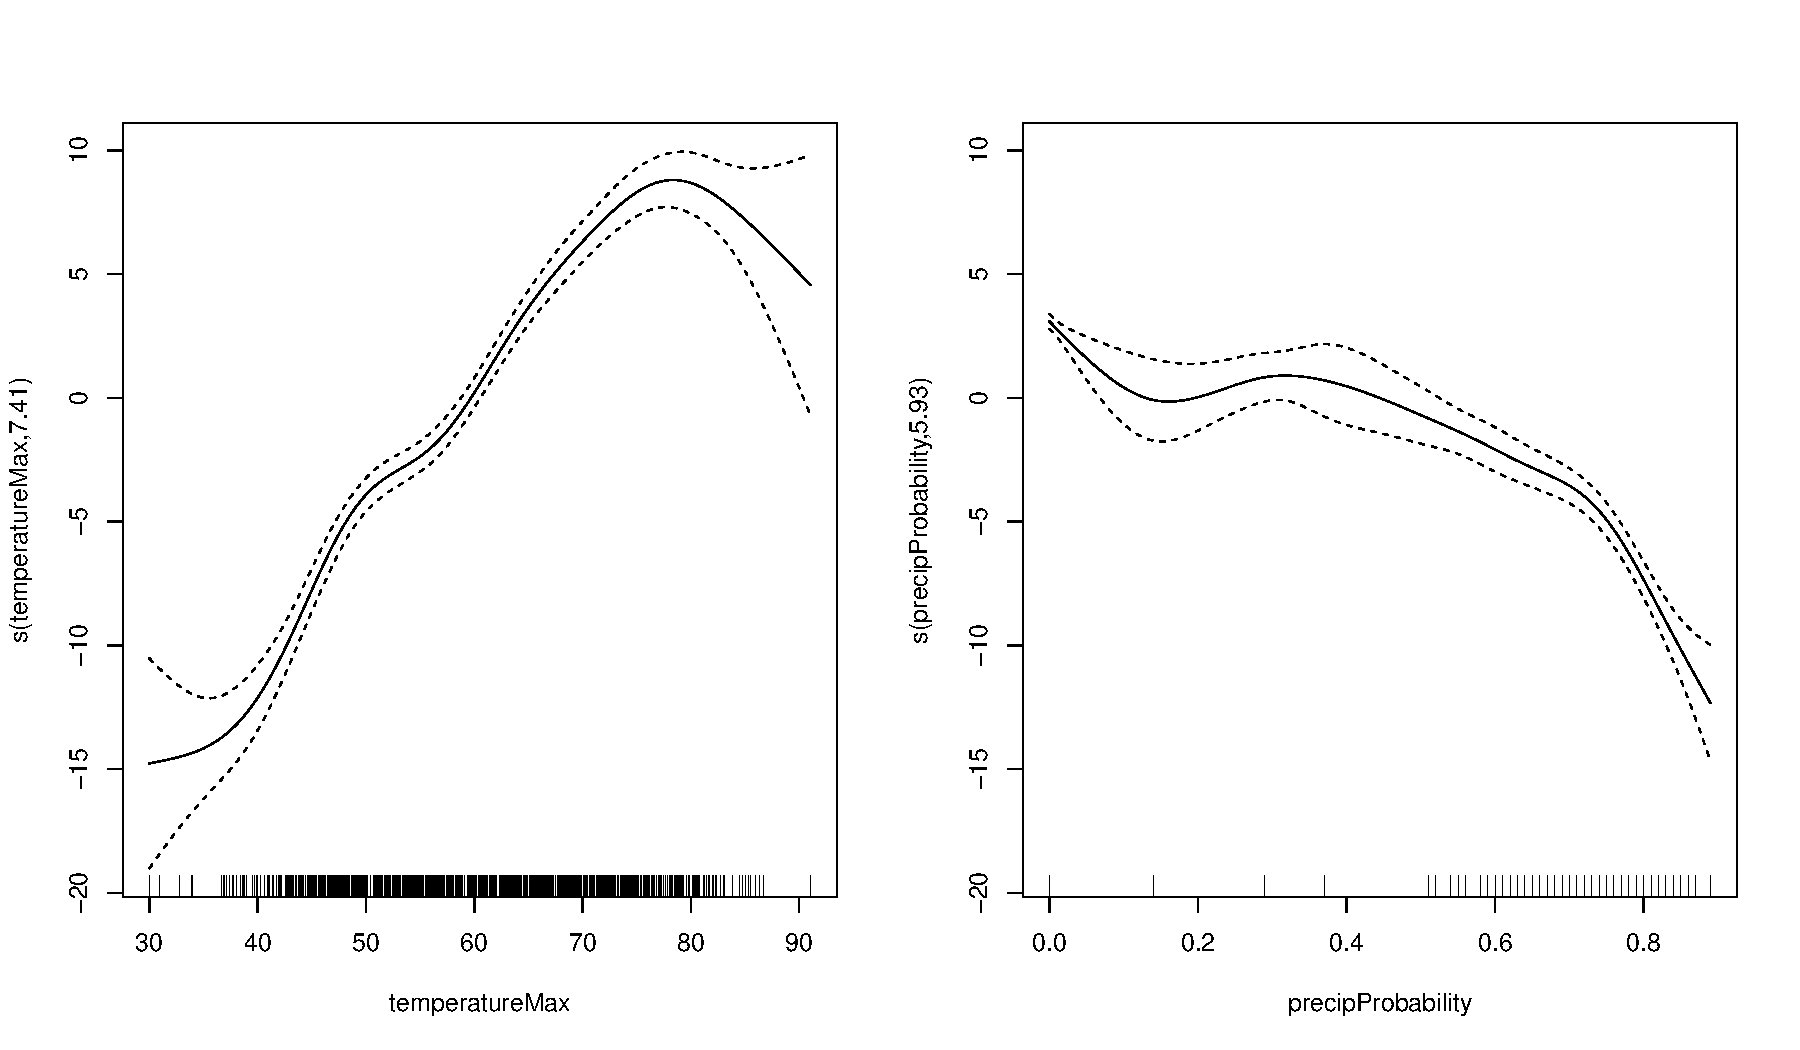
\includegraphics[width=1\textwidth]{figures/gam.pdf} 
\vspace{-10pt}
  \caption{Smooth functions of \texttt{TempMax} and \texttt{PrecipProb}}
  \label{fig:smooth}
\vspace{-1.05cm}
\end{figure}

We are interested to see the form of the smooth function $s_1$ and $s_2$ of temperature and precipitation probability, which will in turn characterize their nonlinear impact on bike counts. As is seen in Figure~\ref{fig:smooth}, the smooth function of \texttt{TempMax} clearly follows an nonlinear relationship. The smooth function $s_1$ provides an accurate characterization of the nonlinear relationship between \texttt{TempMax} and bike counts. It also suggests a quadratic term $\texttt{TempMax}^2$ could be included in the base model to capture the observed nonlinear relationship. Furthermore, GAM helps one to determine the important turning points. When the maximum daily temperature is below $40^{\circ}$F, the bike count will approximately remain the same; when it is in the range of $40^{\circ}$F and $75^{\circ}$, the bike counts monotonically increases as the temperature rises. However, when the max temperature is above $75^{\circ}$F, the bike counts will start drop. It is consistent with finding that is reported in other studies~\cite{Rose07,Richardson00}. Such implications could be used to generate a categorical temperature variable (i.e., low, medium and high) in modeling.

Similarly, the GAM model suggests a nonlinear relationship between \texttt{PrecipProb} and bike counts which is fully characterized by the smooth function $s_2$ as is in Figure~\ref{fig:smooth}. It could be roughly approximated by a piecewise linear function: when the precipitation probability is smaller than 0.75, there is a relatively small negative linear relationship between \texttt{PrecipProb} and bike counts; whereas when \texttt{PrecipProb} becomes higher than 0.75, the bike count will experience the steeper decreasing rate. This finding is interesting in the sense that the utilitarian biker at the Fremont Bridge are likely to ignore rainfall when make biking decisions unless the probability is very high (0.75). It also suggests including a piecewise linear function of the \texttt{PrecipProb} in the model could be helpful to improve performance.

\begin{figure}
\centering
   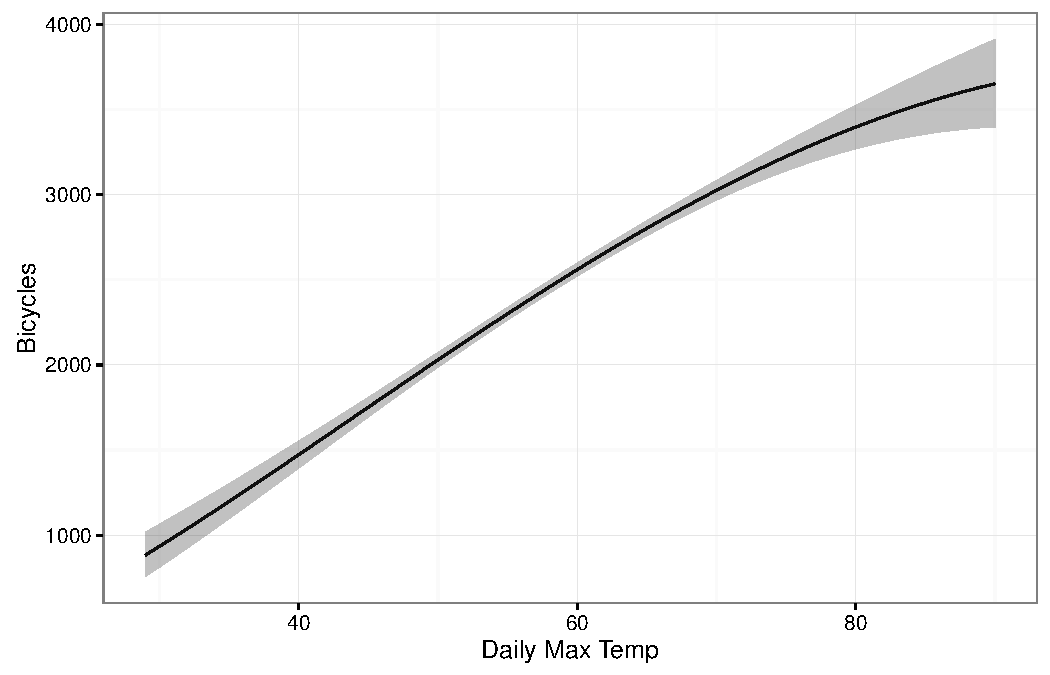
\includegraphics[width=0.7\textwidth]{figures/sim/temperture} 
  \caption{Effect of \texttt{TempMax} on bicycle counts, with shaded 95\% prediction interval.}
  \label{fig:temp}
\end{figure}

Combining the findings in the GAM fit, we first the following model:

\textbf{Model 0}
\begin{align}
\sqrt{\text{Count}_t} &= \beta_0 + \beta_1 \text{TempMax}^2_t + \beta_2 \text{TempMax}_t + \beta_3 \text{Holiday}_t + \beta_4 \text{PrecipProb}_t  \nonumber\\
&\qquad + \beta_5 \text{Weekend}_t + \beta_6 \text{Daylight}_t + \beta_7 \text{UW}_t + \epsilon.\label{eqref:model0}
\end{align}
Model 0 includes the $\texttt{TempMax}^2$ to account for the nonlinearity in temperature on bike counts. The fitted parameter estimates, goodness-of-fit metrics are summarized in Table~\ref{tbl:modelresult_weather}. Each of the coefficients in Model 0 is statistically significant at the $p<0.01$ level. The adjusted $R^2$ of Model 0 is 0.866, which means approximately 87\% of the bike count variance could be explained by the fitted responses of Model 0. 

In order to provide results that are more readily interpretable by non-statisticians, counterfactual simulations are used to isolate individual terms from the model that correspond to our research6 questions. In so doing, we simulated various quantities of interest including point estimates and  confidence intervals,and then plotted them for visual inspection. Figure~\ref{fig:temp} shows that the temperature variable has a clearly positive association with increased number of bicyclists. The nonlinear relationship between temperature and bike counts is accounted for by the squared temperature max term. Such effect is captured in Model 0 as shown in Figure~\ref{fig:temp} where the bike counts start leveling off at very high temperatures (higher than 80$^\circ$F). Because of the relative simplicity, Model 0 serves as the 'base model' in the following discussion. 

\begin{figure}
\centering
   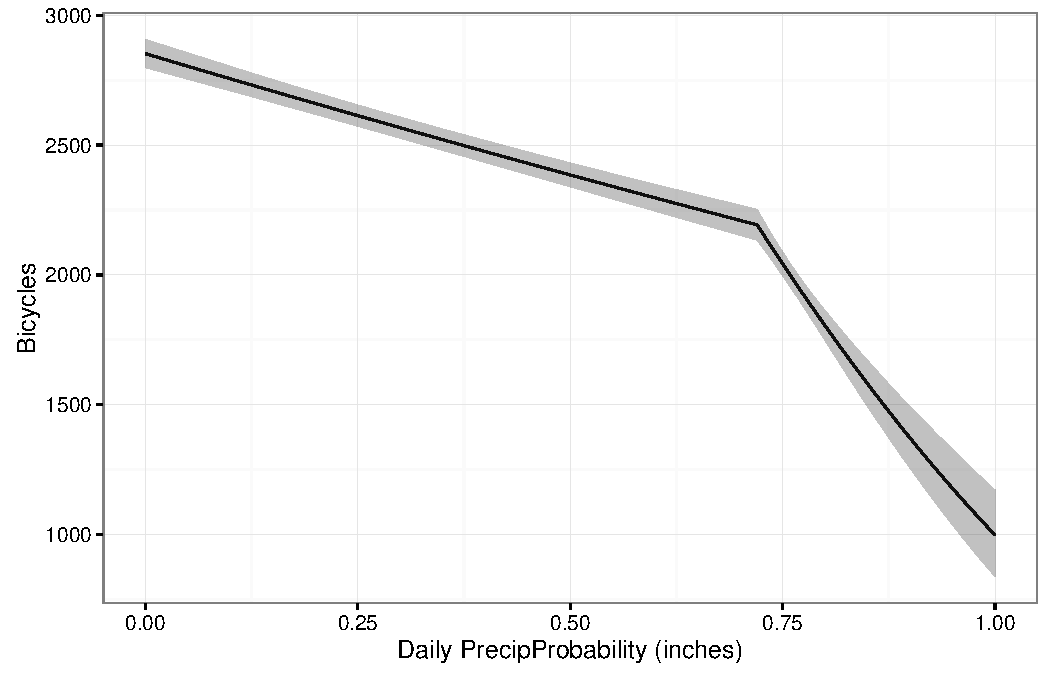
\includegraphics[width=0.7\textwidth]{figures/sim/precip} 
  \caption{Effect of \texttt{PrecipProb} on bicycle counts, with shaded 95\% prediction interval.}
  \label{fig:precip}
\end{figure}

Next we take the nonlinearity in \texttt{PrecipProb} into account by assuming a piecewise linear structure, as suggested by the GAM fit. The alternative model is therefore given by the following:
\textbf{Model 1}
\begin{align}
\sqrt{\text{Count}_t} &= \beta_0 + \beta_1 \text{TempMax}^2_t + \beta_2 \text{TempMax}_t + \beta_3 \text{Holiday}_t + \beta_4 \text{PrecpProb}_t + \beta_5 \text{ppp}_t  \nonumber\\
&\qquad + \beta_5 \text{Weekend}_t + \beta_6 \text{Daylight}_t + \beta_7 \text{UW}_t + \epsilon.\label{eqref:model1}
\end{align}
Model 1 differs Model 0 with the addition of \texttt{pp}, which serves as a calibration term to \texttt{PrecipProb} to make it piecewise linear. \texttt{ppp} is defined as. The fitted parameter estimates, goodness-of-fit metrics are again summarized in Table~\ref{tbl:modelresult_weather}. Each of the coefficients in Model 1 is statistically significant at the $p<0.01$ level. The adjusted $R^2$ also increases to 0.872 from 0.866 in Model 0. The AIC and BIC both suggests a better fitting after accounting for the nonlinearity in \texttt{PrecipProb}. Figure~\ref{fig:precip} shows a clear inverse relationship between precipitation probability and bicycle counts. The rate of decrease in bicycles appears to begin somewhat flat, and then begins to drop steeply at higher probability of precipitation. This suggests that bicyclists won't take the \texttt{PrecipProb} seriously in their decision to ride until it is very high. This could be due to the constant presence of precipitation in Seattle and the inaccuracy of the weather report.

Another weather variable we are interested is the \texttt{Weather} variable. \texttt{Weather} is a general description of the weather condition and it is represented as a dummy variable in the model, such as 'fog', 'cloudy','partly-cloudy-day', etc. The hypothesis behind this is that people may make riding decisions based on the easily perceived weather classification rather than the actual temperature or precipitation number. The alternative model specification is as follows:

\textbf{Model 2}
\begin{align}
\sqrt{\text{Count}_t} &= \beta_0 + \beta_1 \text{TempMax}^2_t + \beta_2 \text{TempMax}_t + \beta_3 \text{Holiday}_t + \beta_4 \text{PrecpProb}_t  \nonumber\\
&\qquad + \beta_5 \text{Weekend}_t + \beta_6 \text{Daylight}_t + \beta_7 \text{Weather}_t  + \beta_8 \text{UW}_t + \epsilon.\label{eqref:model2}
\end{align}
Model 2 differs Model 1 with the addition of \texttt{Weather} variable. Model 2's parameter estimates, goodness-of-fit metrics are summarized in Table~\ref{tbl:modelresult_weather}. Noted that the weather Weathers 'fog', 'wind', 'partly-cloudy-day' and 'partly-cloudy-night' are all found to be not statistically significant at $p<0.1$ level. The adjusted $R^2$ increase is also marginal given the addition of \texttt{Weather} variable. This suggests that simple weather classifications don't have a significant impact on bike counts.

\begin{table}[!htbp] \centering 
  \caption{Results: weather variables} 
  \label{tbl:modelresult_weather} 
\begin{tabular}{@{\extracolsep{-50pt}}lD{.}{.}{-3} D{.}{.}{-3} D{.}{.}{-3} } 
\\[-3ex]\hline 
\hline \\[-4ex] 
 & \multicolumn{3}{c}{\textit{Dependent variable: $\sqrt{\text{Bike Counts}}$}} \\ \cline{2-4} 
\\[-4ex] & \multicolumn{1}{c}{Model 0 (base)} & \multicolumn{1}{c}{Model 1 (precip)} & \multicolumn{1}{c}{Model 2 (Weather)}\\ 
\hline \\[-1.8ex] 
 TempMaxSq & -0.006^{***}$ $(0.001) & -0.006^{***}$ $(0.001) & -0.006^{***}$ $(0.001) \\ 
  TempMax & 1.151^{***}$ $(0.136) & 1.179^{***}$ $(0.133) & 1.127^{***}$ $(0.137) \\ 
  Holiday & -14.680^{***}$ $(0.850) & -14.277^{***}$ $(0.829) & -14.809^{***}$ $(0.840) \\ 
  PrecipProb & -11.734^{***}$ $(0.473) & -9.142^{***}$ $(0.565) & -8.517^{***}$ $(0.763) \\ 
  ppp &  & -45.184^{***}$ $(5.693) &  \\ 
  Weekend & -17.435^{***}$ $(0.316) & -17.277^{***}$ $(0.308) & -17.421^{***}$ $(0.312) \\ 
  daylight & 1.016^{***}$ $(0.088) & 0.946^{***}$ $(0.086) & 1.037^{***}$ $(0.090) \\ 
  cloudy &  &  & -2.956^{***}$ $(1.036) \\ 
  fog &  &  & 0.146$ $(0.702) \\ 
  partly-cloudy-day &  &  & -0.107$ $(0.436) \\ 
  partly-cloudy-night &  &  & 0.579$ $(0.594) \\ 
  rain &  &  & -2.785^{***}$ $(0.561) \\ 
  wind &  &  & -4.159$ $(3.404) \\ 
  UW & 3.272^{***}$ $(0.348) & 3.487^{***}$ $(0.340) & 3.266^{***}$ $(0.344) \\ 
  const. & -3.627$ $(3.796) & -4.775$ $(3.701) & -2.900$ $(3.818) \\ 
 \hline \\[-1.8ex] 
Observations & \multicolumn{1}{c}{1,157} & \multicolumn{1}{c}{1,157} & \multicolumn{1}{c}{1,157} \\ 
R$^{2}$ & \multicolumn{1}{c}{0.866} & \multicolumn{1}{c}{0.873} & \multicolumn{1}{c}{0.870} \\ 
Adjusted R$^{2}$ & \multicolumn{1}{c}{0.866} & \multicolumn{1}{c}{0.872} & \multicolumn{1}{c}{0.869} \\ 
AIC & \multicolumn{1}{c}{6930} & \multicolumn{1}{c}{6870} & \multicolumn{1}{c}{6906} \\ 
BIC & \multicolumn{1}{c}{6976} & \multicolumn{1}{c}{6921} & \multicolumn{1}{c}{6982} \\  
\hline 
\hline \\[-1.8ex] 
\textit{Note:}  & \multicolumn{3}{r}{$^{*}$p$<$0.1; $^{**}$p$<$0.05; $^{***}$p$<$0.01} \\ 
\end{tabular} 
\end{table} 


\subsection{Seasonal Impact}
In Model 0, four variables are considered to the effect of seasonality on bicyclist counts: the first being the number of daylight hours, the second being whether or not the University of Washington (proxying more generally for other educational institutions) was in session, third being the holiday indicator \texttt{Holiday}, and the fourth being the weekend indicator \texttt{Weekend}.

Figure~\ref{fig:daylightuw} shows that we see a substantial increase in bicycle volume when the UW is in session. With all other factors held constant we see that, on days when the university is in session, we would expect an average of approximately 367 additional bicycle observed. Similarly, we see a rougly linear increase in bicycles with increased day length.

\begin{figure}
\centering
   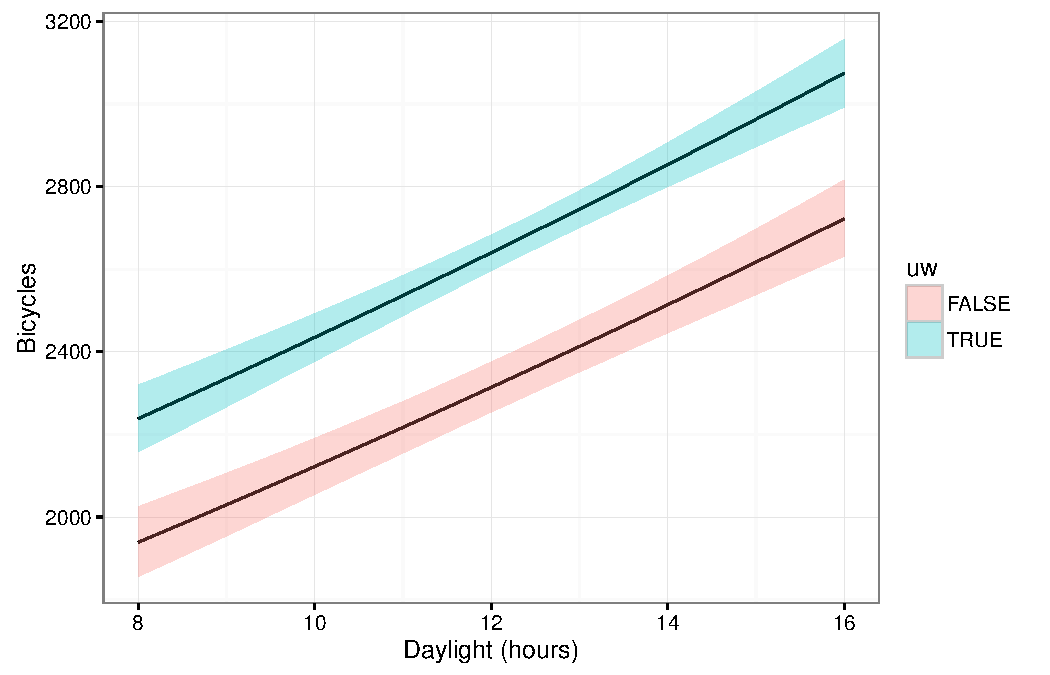
\includegraphics[width=0.7\textwidth]{figures/sim/daylight} 
  \caption{Effect of \texttt{Daylight} and \texttt{UW} in-session status on bicycle counts, with shaded 95\% prediction interval.}
  \label{fig:daylightuw}
\end{figure}

\begin{figure}
\centering
  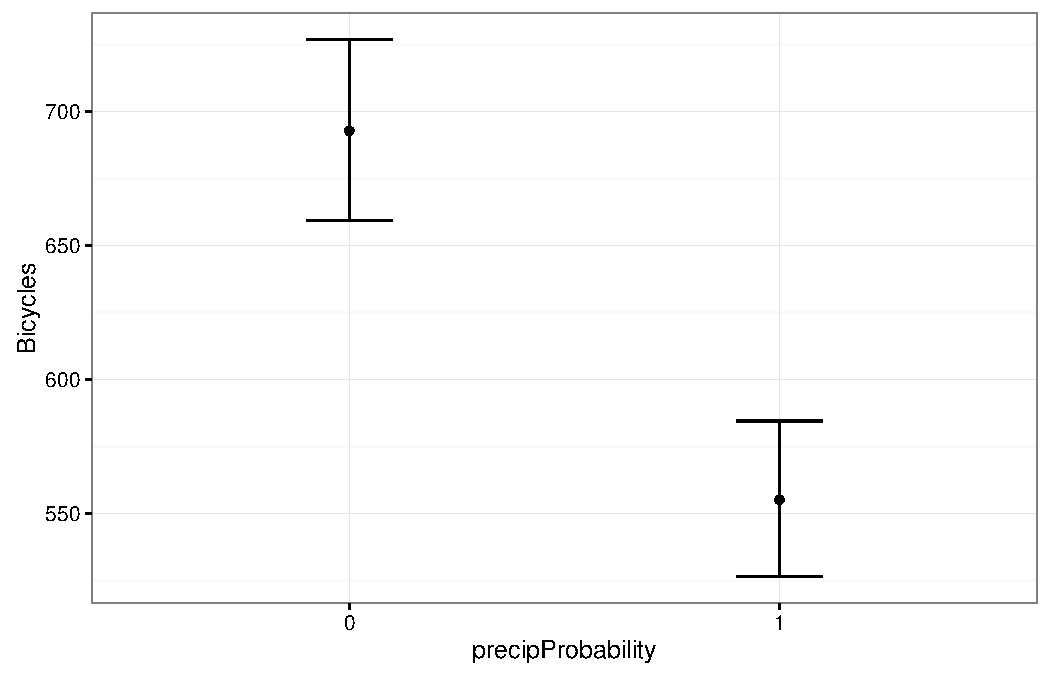
\includegraphics[width=0.7\textwidth]{figures/sim/Wknd}
%   \includegraphics[width=0.7\textwidth]{figures/sim/wknd_cat}  
  \caption{Effect of \texttt{weekend} on bicycle counts, with shaded 95\% prediction interval.}
  \label{fig:weekend}
\end{figure}

Figure~\ref{fig:holiday} and Figure~\ref{fig:weekend} shows the impact of the holiday and weekend on the bike counts. In both cases, when the date of interest is a holiday or weekend, there is lower number of bicycle counts compared to a non-holiday, weekend. This strongly suggests that the majority of the bicycle traffic at this location is for utilitarian purpose. 

% \begin{figure}
% \centering
%   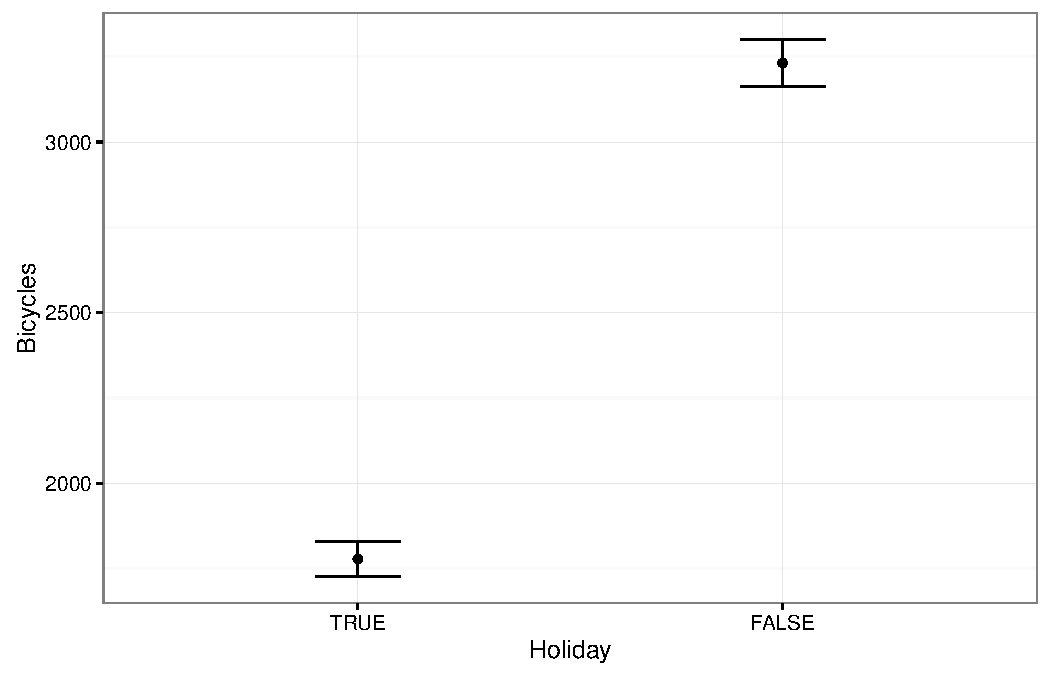
\includegraphics[width=0.7\textwidth]{figures/sim/holiday} 
%  \caption{Effect of \texttt{holiday} on bicycle counts, with shaded 95\% prediction interval.}
%  \label{fig:holiday}
% \end{figure}

\begin{figure}
\centering
  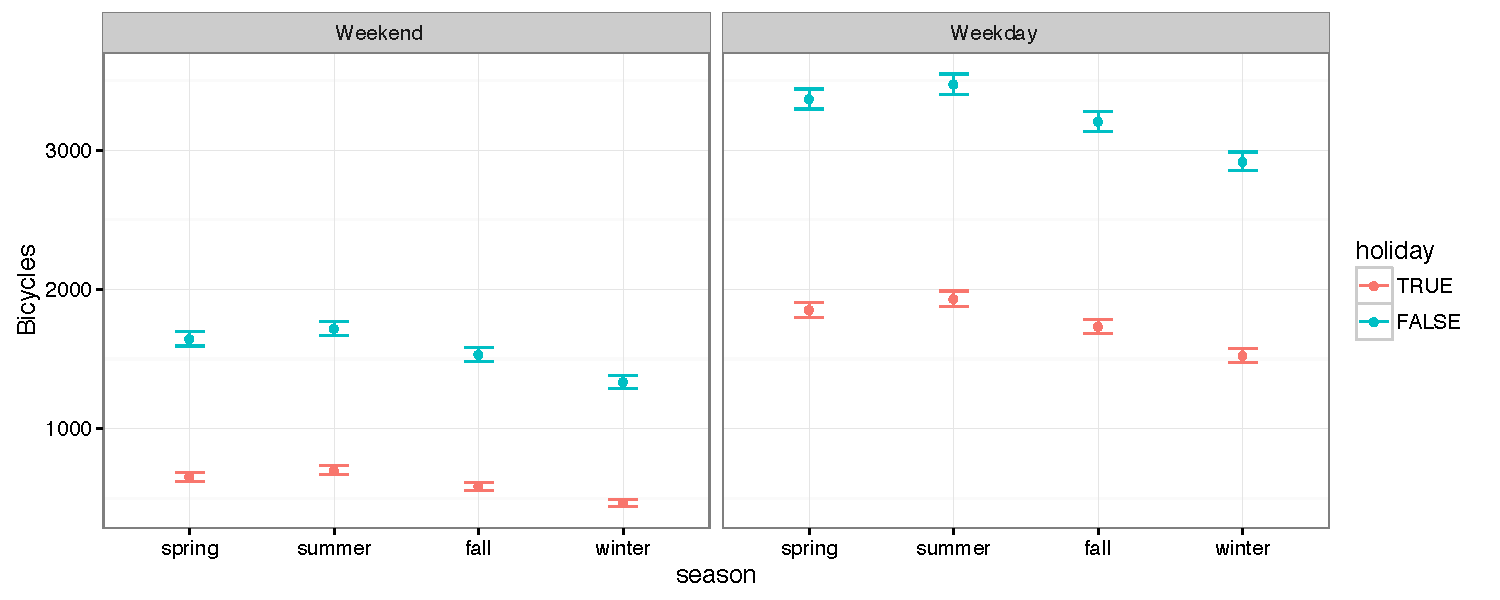
\includegraphics[width=1\textwidth]{figures/sim/multi} 
 \caption{Effect of \texttt{holiday} on bicycle counts, with shaded 95\% prediction interval.}
 \label{fig:multi}
\end{figure}


Several additional alternative seasonal variables are considered for model specifications. In Model 0,  the continuously-valued variable \texttt{daylight} is considered to account for the yearly seasonality (see Figure~\ref{fig:daylight}). In the following, it is replaced by the \texttt{season} which is a dummy variable that take value in 'winter','spring' and 'summer' ('autumn' serves as the reference and thus omitted). The alternative model specification is given by:

\textbf{Model 3}
\begin{align}
\sqrt{\text{Count}_t} &= \beta_0 + \beta_1 \text{TempMax}^2_t + \beta_2 \text{TempMax}_t + \beta_3 \text{Holiday}_t + \beta_4 \text{PrecpProb}_t  \nonumber\\
&\qquad + \beta_5 \text{Weekend}_t + \beta_6 \text{Season}_t + \beta_6 \text{UW}_t + \epsilon.\label{eqref:model3}
\end{align}
Model 3 replaces the \texttt{Daylight} hours in Model 0 by the \texttt{Season} . Model 3's parameter estimates, goodness-of-fit metrics are summarized in Table~\ref{tbl:modelresult_seasonal}. All coefficients of the season variables appear to be  statistically significant in Model 3 at the $p<0.01$ level. The adjusted $R^2$ is slightly lower than Model 0. Figure~\ref{fig:season} shows that there is generally more bike counts in summer time than winter.

\begin{figure}
\centering
  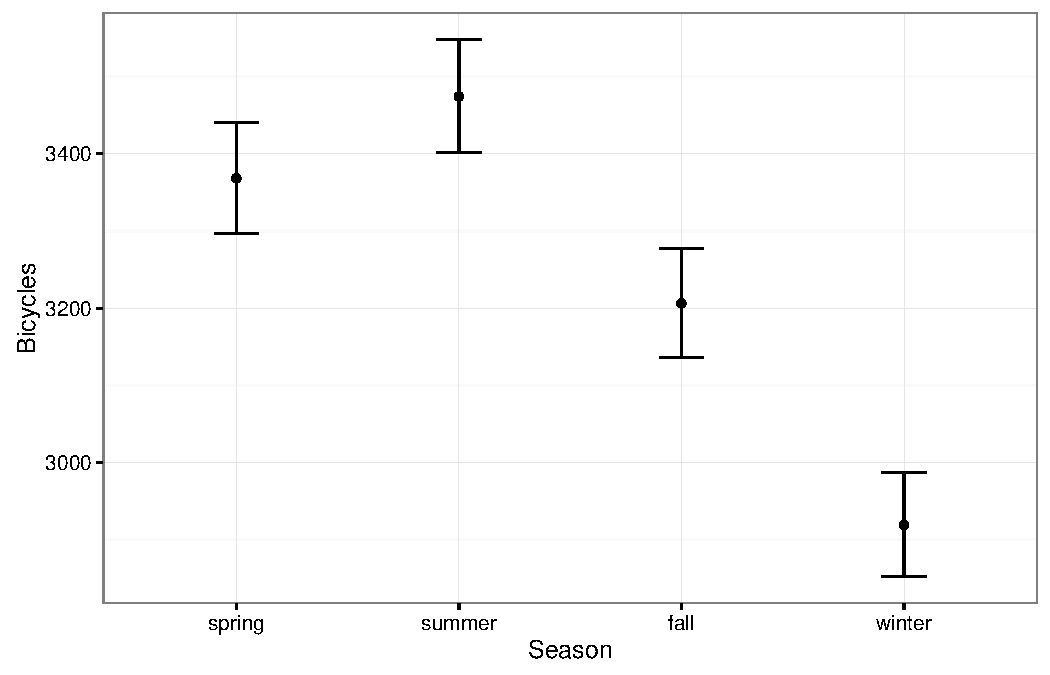
\includegraphics[width=0.7\textwidth]{figures/sim/season} 
 \caption{Effect of \texttt{Season} on bicycle counts, with shaded 95\% prediction interval.}
 \label{fig:season}
\end{figure}

Next we consider the \texttt{Weekend} variable substituted by the day of week variable \texttt{dow}. The use of \texttt{dow} has been documented a lot in the literature~\cite{Miranda-Moreno:2011aa,Ahmed12}. It is included as a dummy variable, such as 'Saturday', 'Sunday','Monday','Tuesday','Wednesday' and 'Thursday' ('Friday' serves as the reference and therefore omitted). It is included to account for the weekly variation in bicycle counts apparent in timeseries plot. The alternative model specification is given by:

\textbf{Model 4}
\begin{align}
\sqrt{\text{Count}_t} &= \beta_0 + \beta_1 \text{TempMax}^2_t + \beta_2 \text{TempMax}_t + \beta_3 \text{Holiday}_t + \beta_4 \text{PrecpProb}_t \nonumber\\
&\qquad + \beta_5 \text{dow}_t  + \beta_6 \text{Daylight}_t + \beta_7 \text{UW}_t + \epsilon.\label{eqref:model4}
\end{align}
Model 4 replaces \texttt{Weekend} variable in Model 0 by \texttt{dow} variable. Model 4's parameter estimates, goodness-of-fit metrics are summarized in Table~\ref{tbl:modelresult_seasonal}. Figure~\ref{fig:dow} shows several interesting aspects of these results. First, we see much higher number of bicyclists on weekdays than on weekends. Then comparing between weekday results, we see that most days are roughly the same, with Tuesday having the most bike traffic and Friday the least. This decrease toward the end of work week might be attributable to individuals either working non-traditional schedules or perhaps people adjusting their travel mode choice in order to accomodate social engagements. Despite the small changes in weekday counts, the weekend/weekday difference is more significant and we believe it is sufficient to include the \texttt{Weekend} variable in our model for explanation purpose.

\begin{figure}
\centering
   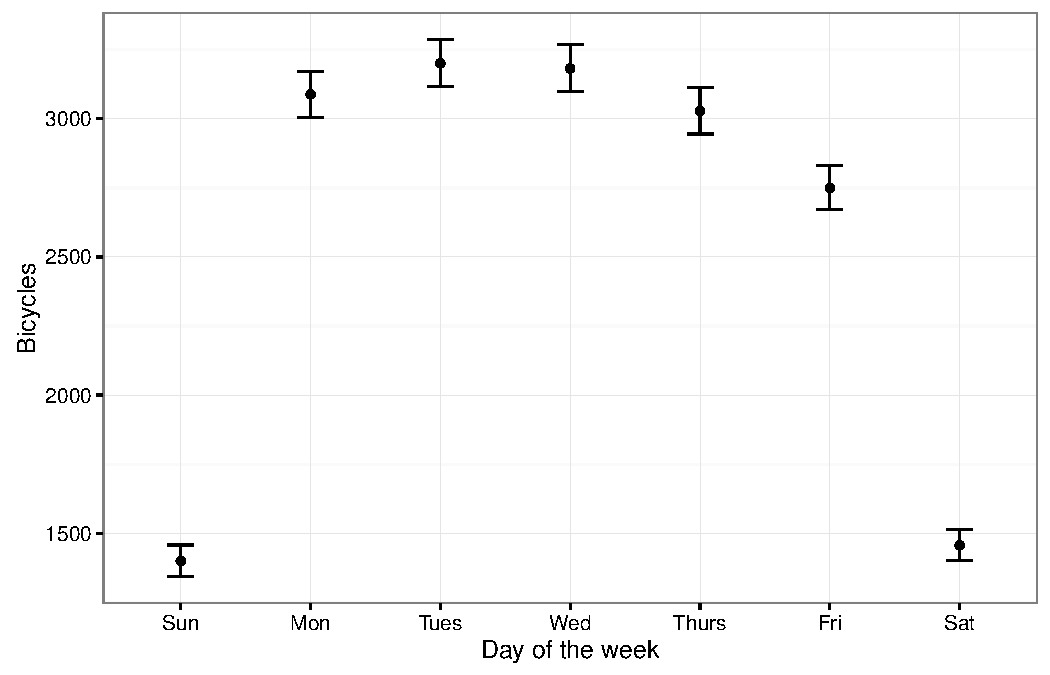
\includegraphics[width=0.7\textwidth]{figures/sim/dow} 
  \caption{Effect of \texttt{dow} on bicycle counts, with shaded 95\% prediction interval.}
  \label{fig:dow}
\end{figure}

\begin{table}[!htbp] \centering 
  \caption{Results: Seasonal factors} 
  \label{tbl:modelresult_seasonal} 
\begin{tabular}{@{\extracolsep{-60pt}}lD{.}{.}{-3} D{.}{.}{-3} D{.}{.}{-3} } 
\\[-3ex]\hline 
\hline \\[-4ex] 
 & \multicolumn{3}{c}{\textit{Dependent variable: $\sqrt{\text{Bike Count}}$ }} \\
\cline{2-4} 
\\[-4ex] & \multicolumn{1}{c}{Model 0 (base)} & \multicolumn{1}{c}{Model 3 (season)} & \multicolumn{1}{c}{Model 4 (dow)}\\ 
\hline \\[-1.8ex] 
 TempMaxSq & -0.006^{***}$ $(0.001) & -0.006^{***}$ $(0.001) & -0.005^{***}$ $(0.001) \\ 
  TempMax & 1.151^{***}$ $(0.136) & 1.167^{***}$ $(0.132) & 1.190^{***}$ $(0.149) \\ 
  Holiday & -14.680^{***}$ $(0.850) & -14.424^{***}$ $(0.827) & -14.985^{***}$ $(0.874) \\ 
  PrecipProb & -11.734^{***}$ $(0.473) & -11.725^{***}$ $(0.457) & -12.205^{***}$ $(0.481) \\ 
  Weekend & -17.435^{***}$ $(0.316) &  & -17.483^{***}$ $(0.324) \\ 
  Sat &  & -14.271^{***}$ $(0.514) &  \\ 
  Sun &  & -15.035^{***}$ $(0.514) &  \\ 
  Mon &  & 3.135^{***}$ $(0.514) &  \\ 
  Tue &  & 4.140^{***}$ $(0.513) &  \\ 
  Wed &  & 3.970^{***}$ $(0.512) &  \\ 
  Thu &  & 2.589^{***}$ $(0.511) &  \\ 
  daylight & 1.016^{***}$ $(0.088) & 1.016^{***}$ $(0.085) &  \\ 
  winter &  &  & -2.592^{***}$ $(0.492) \\ 
  spring &  &  & 1.413^{***}$ $(0.417) \\ 
  summer &  &  & 2.320^{***}$ $(0.543) \\ 
  UW & 3.272^{***}$ $(0.348) & 3.329^{***}$ $(0.336) & 3.242^{***}$ $(0.384) \\ 
  const. & -3.627$ $(3.796) & -6.969^{*}$ $(3.692) & 5.635$ $(4.491) \\ 
 \hline \\[-1.8ex] 
Observations & \multicolumn{1}{c}{1,157} & \multicolumn{1}{c}{1,157} & \multicolumn{1}{c}{1,157} \\ 
R$^{2}$ & \multicolumn{1}{c}{0.866} & \multicolumn{1}{c}{0.876} & \multicolumn{1}{c}{0.860} \\ 
Adjusted R$^{2}$ & \multicolumn{1}{c}{0.866} & \multicolumn{1}{c}{0.875} & \multicolumn{1}{c}{0.859} \\ 
AIC & \multicolumn{1}{c}{6930} & \multicolumn{1}{c}{6855} & \multicolumn{1}{c}{6989} \\ 
BIC & \multicolumn{1}{c}{6976} & \multicolumn{1}{c}{6926} & \multicolumn{1}{c}{7045} \\ 
\hline 
\hline \\[-1.8ex] 
\textit{Note:}  & \multicolumn{3}{r}{$^{*}$p$<$0.1; $^{**}$p$<$0.05; $^{***}$p$<$0.01} \\ 
\end{tabular} 
\end{table}

\subsection{Interact Relationship}
Interaction effects among weather variables (e.g., combined effect of temperature and humidity) on the bike count have been studied in the literature~\cite{Miranda-Moreno:2011aa}. However, few attention is given to interactions between weather variables and seasonal factors, although such interaction has been noticed in the literature~\cite{Thomas12}. In~\cite{Thomas12}, it is concluded cycling on utilitarian facilities is more sensitive to weather conditions on weekends. In this alternative model specification, the interaction term between \texttt{Weekend} and \texttt{PrecipProb} is considered:

\textbf{Model 5}
\begin{align}
\sqrt{\text{Count}_t} &= \beta_0 + \beta_1 \text{TempMax}^2_t + \beta_2 \text{TempMax}_t + \beta_3 \text{Holiday}_t + \beta_4 \text{PrecpProb}_t \nonumber\\
&\qquad +\beta_5 \text{Weekend}_t  + \beta_6 \text{PrecpProb}_t \times \text{Weekend}_t + \beta_7\text{Daylight}_t + \beta_8 \text{UW}_t + \epsilon. \label{eqref:model5}
\end{align}
Model 5 differs from Model 0 by allowing interactions between \texttt{PrecipProb} and \texttt{Weekend}. Model 5's parameter estimates, goodness-of-fit metrics are summarized in Table~\ref{tbl:modelresult_interaction}. The coefficient for the interaction term is significant and with a negative value. This indicates that during weekends, the \texttt{PrecipProb} has a bigger negative effect on bike counts. This could be due to most bicyclists on weekends are recreational and thus more sensitive to weather conditions. The impact of \texttt{Weekend} and \texttt{PrecipProb} on bike counts are illustrated in Figure~\ref{fig:interact}.

\begin{figure}
\centering
   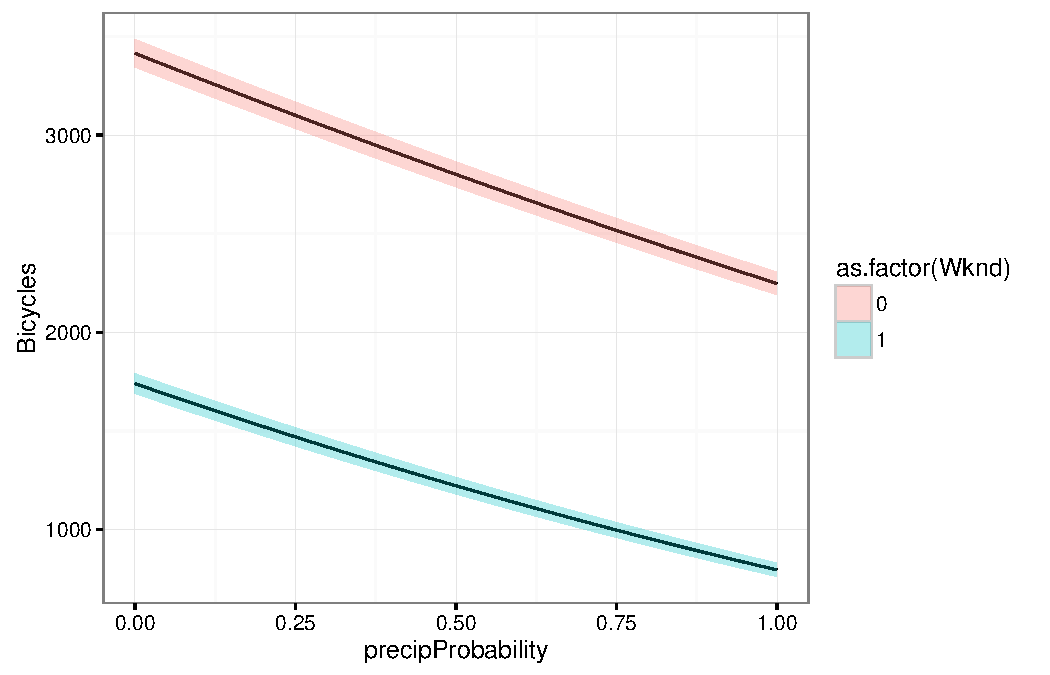
\includegraphics[width=0.7\textwidth]{figures/sim/interact} 
  \caption{Effect of \texttt{Weekend} and \texttt{PrecipProb} on bicycle counts, with shaded 95\% prediction interval.}
  \label{fig:interact}
\end{figure}

\subsection{Trend analysis}
To test for a linear trend in bicycle volumes, we include a time index variable \texttt{T} in the model. We created this variable by sequentially numbering (1-1157) the observed counts by day during the study period. The alternative model specification is as follows:

\begin{figure}
\centering
   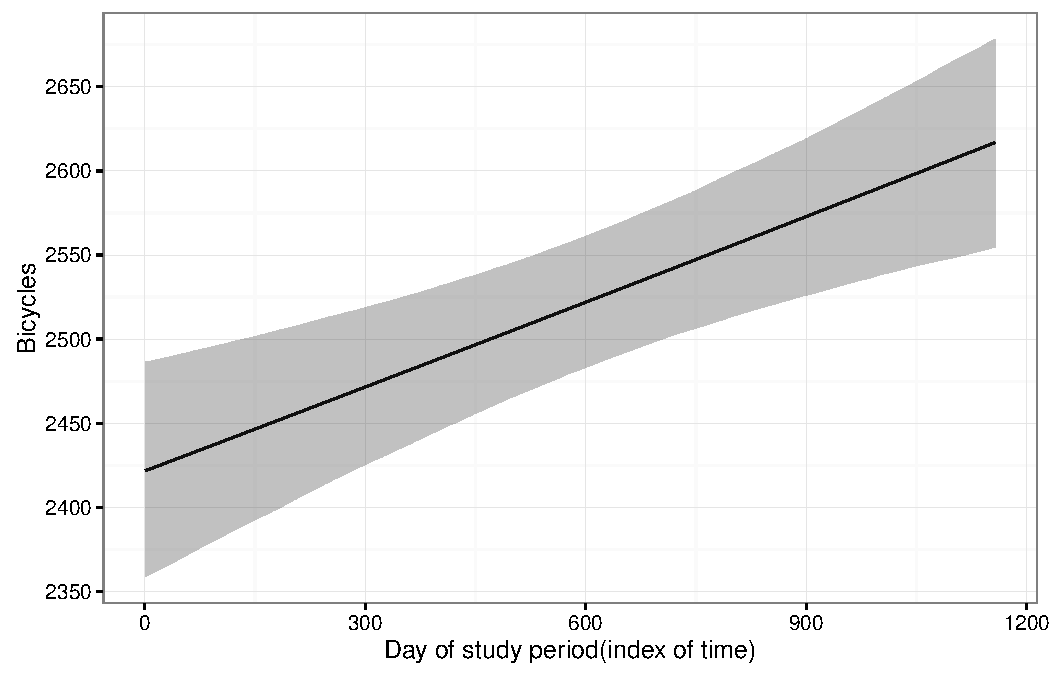
\includegraphics[width=0.7\textwidth]{figures/sim/trend} 
  \caption{General trend in bicycling counts, all other factors held constant, with 95\% confidence region.}
  \label{fig:trend}
\end{figure}

\begin{table}[!htbp] \centering 
  \caption{Results: Interaction and Trend} 
  \label{tbl:modelresult_interaction} 
\begin{tabular}{@{\extracolsep{-50pt}}lD{.}{.}{-3} D{.}{.}{-3} D{.}{.}{-3} } 
\\[-3ex]\hline 
\hline \\[-4ex] 
 & \multicolumn{3}{c}{\textit{Dependent variable:$\sqrt{\text{Bike Count}}$}} \\ 
\cline{2-4} 
\\[-4ex] & \multicolumn{1}{c}{Model 0 (base)} & \multicolumn{1}{c}{Model 5 (interaction)} & \multicolumn{1}{c}{Model 6 (trend)}\\ 
\hline \\[-1.8ex] 
 TempMaxSq & -0.006^{***}$ $(0.001) & -0.006^{***}$ $(0.001) & -0.005^{***}$ $(0.001) \\ 
  TempMax & 1.151^{***}$ $(0.136) & 1.163^{***}$ $(0.136) & 1.087^{***}$ $(0.136) \\ 
  Holiday & -14.680^{***}$ $(0.850) & -14.663^{***}$ $(0.848) & -14.690^{***}$ $(0.845) \\ 
  PrecipProb & -11.734^{***}$ $(0.473) & -11.027^{***}$ $(0.541) & -11.659^{***}$ $(0.471) \\ 
  Weekend & -17.435^{***}$ $(0.316) & -16.722^{***}$ $(0.413) & -17.441^{***}$ $(0.314) \\ 
  daylight & 1.016^{***}$ $(0.088) & 1.015^{***}$ $(0.088) & 1.079^{***}$ $(0.089) \\ 
  UW & 3.272^{***}$ $(0.348) & 3.263^{***}$ $(0.347) & 3.266^{***}$ $(0.346) \\ 
  PrecipProb:Wknd &  & -2.482^{***}$ $(0.929) &  \\ 
  X &  &  & 0.002^{***}$ $(0.0004) \\ 
  const. & -3.627$ $(3.796) & -4.144$ $(3.791) & -2.817$ $(3.780) \\ 
 \hline \\[-1.8ex] 
Observations & \multicolumn{1}{c}{1,157} & \multicolumn{1}{c}{1,157} & \multicolumn{1}{c}{1,157} \\ 
R$^{2}$ & \multicolumn{1}{c}{0.866} & \multicolumn{1}{c}{0.867} & \multicolumn{1}{c}{0.868} \\ 
Adjusted R$^{2}$ & \multicolumn{1}{c}{0.866} & \multicolumn{1}{c}{0.866} & \multicolumn{1}{c}{0.867} \\ 
AIC & \multicolumn{1}{c}{6930} & \multicolumn{1}{c}{6925} & \multicolumn{1}{c}{6918} \\ 
BIC & \multicolumn{1}{c}{6976} & \multicolumn{1}{c}{6975} & \multicolumn{1}{c}{6968} \\ 
\hline 
\hline \\[-1.8ex] 
\textit{Note:}  & \multicolumn{3}{r}{$^{*}$p$<$0.1; $^{**}$p$<$0.05; $^{***}$p$<$0.01} \\ 
\end{tabular} 
\end{table} 

\textbf{Model 6}
\begin{align}
\sqrt{\text{Count}_t} &= \beta_0 + \beta_1 \text{TempMax}^2_t + \beta_2 \text{TempMax}_t + \beta_3 \text{Holiday}_t + \beta_4 \text{PrecpProb}_t \nonumber\\
&\qquad +\beta_5 \text{Weekend}_t  + \beta_6 \text{daylight}_t + \beta_7 \text{UW}_t + \beta_8\text{day}_t + \epsilon. \label{eqref:model6}
\end{align}
Model 6 differs from Model 0 by the addition of \texttt{T}. Model 6's parameter estimates, goodness-of-fit metrics are summarized in Table~\ref{tbl:modelresult_interaction}. Results shown in Figure~\ref{fig:trend} confirm the presence of a general trend toward increased numbers of bicycles at this location. With all else held constant, we would expect to see roughly 200 more bicycles on days at the end of our study period than at the beginning. This is consistent with figures
reported elsewhere that suggest that bicycling is increasing in a number of cities including Seattle~\cite{League-of-American-Bicyclists:aa}.


As is shown in Table~\ref{tbl:modelresult_weather}-Table~\ref{tbl:modelresult_interaction}, all seven models have a similiar performance in terms of coefficient significance, adjusted $R^2$, AIC and BIC. After balancing model accuracy and simplicity, we will focus on the `base' Model, Model 0, for the following analysis. 

%All fitted models confirm that the bicycle counts have a strong postive relationship with temperature, and a negative relationship with precipitation probability. During weekend and holiday, there is a significant drop in the bike counts. This makes sense since the Fremont bridge is primary a utilitarian bike facility. The daylight, or the seasons, are included to account for the seasonality in the bike count time series. With longer daylight, a larger daily bike count is observed.  
%
%Among five models that are considered, Model 3 has the highest $R^2$, adjusted $R^2$, and the smalledst AIC and BIC values. It could be due to the fact in Model 3, the interaction item (PrecipProb:Wknd) is included to account for the nonlinear relationship between bike counts and those two factors: rather than assuming the bike count depends on the precipitation probability and weekend indicator in an independent fashion, Model 3 assumes the combination of the two jointly impact on bike ridership. This makes sense sincde for utilitarian bicyclist, it is very likely if it rains AND it is weekend, they won't go out biking, whereas in the weekdays, they will still travel even if it's rainy. For simplicity, the weekend indicator is included to substitute the day of week variable. A $R^2$ value of 0.832 indicates that 83.2\% of the variance in the bike count datasets is explained by the model fitted values. 
%
%\textbf{To do: include model interpretation? Make model recommendation?}

% \newpage
% \thispagestyle{empty}
% \mbox{}


\section{Predicative Model}

In this section, we are interested in developing a predicative model for daily bike demand using weather conditions and seasonal factors as covariates. An accurate predicative model is useful to help transportation administrator to make better-informed decisions/preparations in case of inclement weather or special holidays. To better account for the seasonality, we substitute the \texttt{Weekend} variable in Model 0 with the \texttt{dow} in the following prediction models since we believe \texttt{dow} is able to explain more variation in the predicted data. Next we investigate the prediction results of the four OLS regression-based models as discussed in Section~\ref{sec:choiceofmodel}. To quantify their predicative performance, an out-of-sample root mean squared error is calculated and compared against each other. The actual vs. predicted plot is also used to visualize the predication result. In the last part of this section, a time series analysis approach is adopted to improve the prediction performance. An Autoregressive Integrated Moving Average (ARIMA) model is proposed to better account for autocorrelaiton patterns that are observed in the error terms. The results of ARIMA is interpreted. A review on the general ARIMA methodolgoy is provided in Section~\ref{arimaintro}.

\subsection{Predicative Performance Comparison of regression-based models}
We first use regression based models to predict daily bike volumes through the Fremont bridge. The standard linear regression, exponential model, quadratic model and the Poisson model as described in~\ref{sec:choiceofmodel} are applied. To compare their predictive performance, an out-of-sample validation framework is used: each model is trained using only the first two years' data, and the trained model is then used to predict the third year's bike count and compared to the test data set. The root mean squared error is calculated as follows:
\begin{equation*}
\text{rmse} = \sqrt{\frac{1}{N}(\hat{Y}_i - Y_i)^2}
\end{equation*}
where $Y_i$ is the actual bike count at date $i$ in the test data set, $\hat{Y}_i$ is the corresponding predicted bike counts, and $N$ is the number of data points in the data set. The root mean squared error of the four proposed models are reported in Table~\ref{tbl:pred4model}.

\begin{table}
 \centering 
  \label{tbl:pred4model} 
\small
\begin{tabular}{ c | c } 
\hline 
  Name & rmse \\ 
\hline
  Standard linear regression & 595.05  \\ 
  Exponential model ($\log{Y}$) & 631.11 \\ 
  Quadratic model ($\sqrt{Y}$) & 575.89\\ 
  Poisson model & 585.32 \\
\hline 
\end{tabular} 
\caption{Predication performance on test sets in terms of RMSE, using the first two years' data as training data set} 
\end{table} 

% \textbf{Could also calculate the std of errors, or consider different training/test data sets}

Out of the four models, the quadratic model has the smallest RMSE of 575.89. Furthermore, the predicted bike volumes are relatively close to the actual data and most of the variation is predicted, as is shown in Figure~\ref{fig:avpmodel0}, although there are some points that are under-predicted (the bottom left corner). While this error is perhaps too large for many operational uses, observed daily bike volume spans from 0 two 6000 (as is seen in Figure~\ref{fig:avpmodel0}), making a prediction with this level of accuracy is quite useful for strategic decisions about network expansion.
\begin{figure*}
\centering
   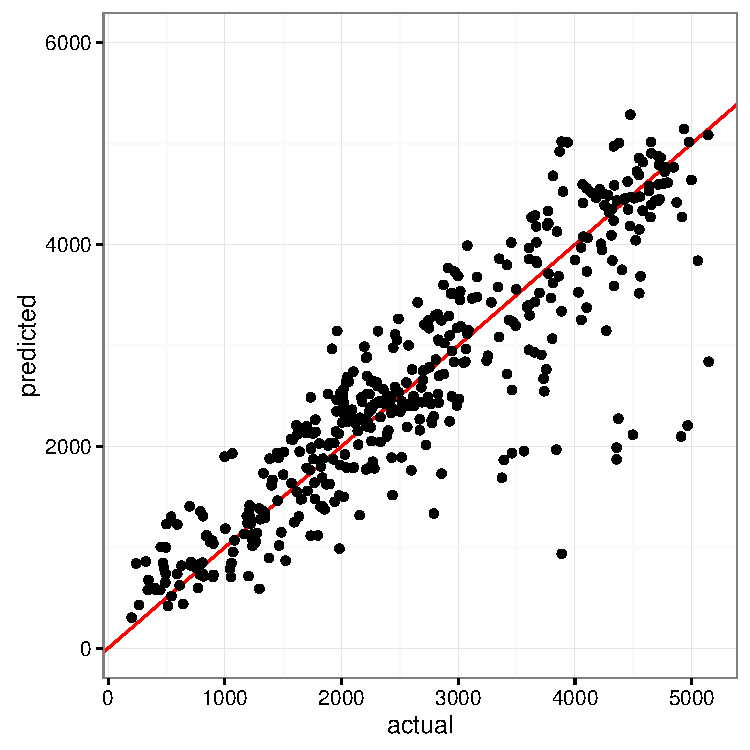
\includegraphics[width=0.7\textwidth]{figures/actualvspred} 
  \caption{Actual vs. predicted daily bike volume. The red line shows actual count is equal to predicted. This plot shows the majority variation is predicted, with some points under-predicted possibly due to special event.}
  \label{fig:avpmodel0}
  \vspace{-.5in}
\end{figure*}




\subsection{Time series analysis with ARIMA model}

In this section, we seek to improve the predicative performance of quadratic model by adopting a time series analysis approach. More specifically, an ARIMA type model is proposed to account for the autocorrelation patterns observed in the OLS regression model error terms. Following the Box-Jenkins approach~\cite{Jenkins70}, we first check the stationarity of the model residual errors. As is shown in the top left plot in Figure~\ref{fig:residual_acfpcf}, there is no discernible long-run trend or seasonality in the residual responses. To confirm this, two statistical stationarity tests are conducted: the Augmented Dickey-Fuller (ADF) test and the Kwiatkowski-Phillips-Schmidt-Shin (KPSS) test. Their results are summarized in Table~\ref{tbl:stationarytest}. Using a significant level of 0.01, these two tests suggest the error terms are stationary.

\begin{table}
 \centering 
  \label{tbl:stationarytest} 
\small
\begin{tabular}{ c | c | c} 
\hline 
  Test Name & $p-$value & Null Hypothesis \\ 
\hline
  ADF test  & 0.01  &  Non-Stationary \\ 
  KPSS test & 0.02 & Stationary \\ 
\hline 
\end{tabular} 
\caption{Statistical stationarity tests with their $p-$values and null hypothesis} 
\vspace{-.2in}
\end{table} 

The autocorrlation plot (ACF) and partial autocorrelation plot (PACF) are then used to examine any possible autocorrelation in the model residuals, as are shown in Figure~\ref{fig:residual_acfpcf}. Recall that an ACF plot shows the autocorrelation which measure the relationship between $Y_t$ and $Y_{t-k}$ for different values of $k$.  The PACF measures the relationship between $Y_t$ and $Y_{t-k}$ after removing the effects of other time lags in between: $1, 2, 3, \hdots, k-1$. The ACF and PACF plots on the left side suggest there is significant autocorrelation in the error terms.

\begin{figure*}
   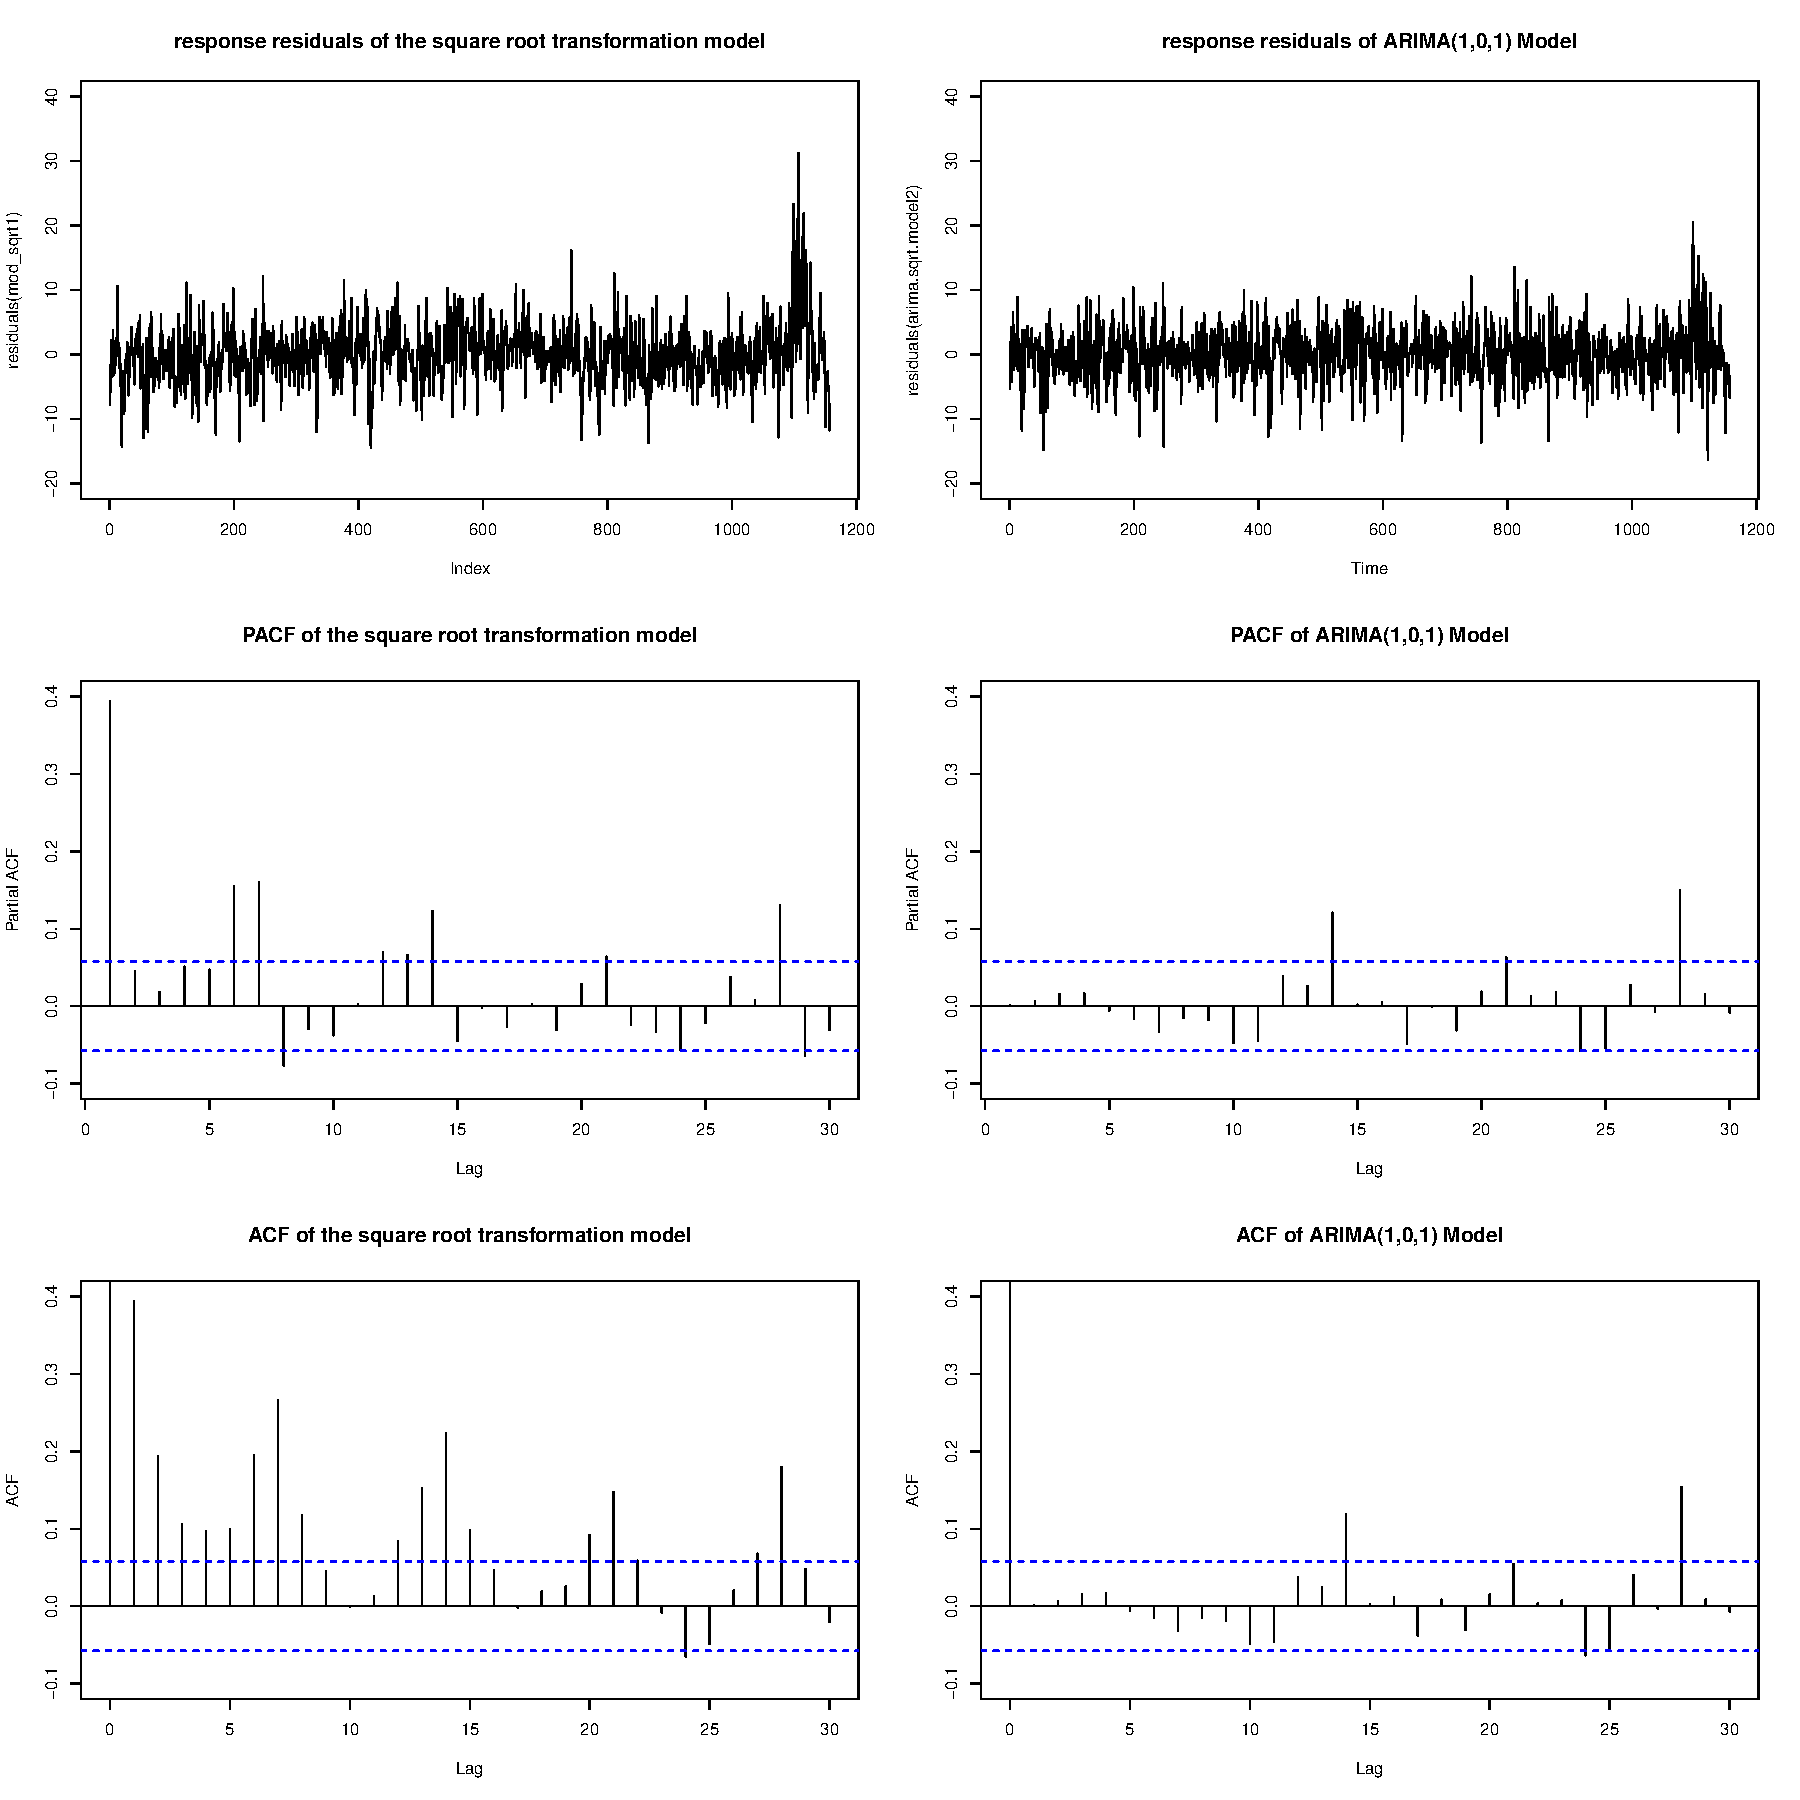
\includegraphics[width=1\textwidth]{figures/residual_acfpcf} 
  \caption{From top to bottom: the residual plots, ACF and PACF of the quadratic model with ARIMA error terms (right) and without ARIMA error terms (left).}
  \label{fig:residual_acfpcf}
\end{figure*}


Noticing that both ACF and PACF of the residual responses (see middle and bottom left plots in Figure~\ref{fig:residual_acfpcf}) have persistent spikes that do not disappear after certain lags, this suggest the order of autoregressive and moving average $(p,q)$ are positive. In this case, the ACF and PACF are not helpful in finding the suitable values of $p$ and $q$. To determine the appropriate order of ARIMA terms, we use the \texttt{auto.arima} function of \texttt{forecast} package in \texttt{R} to aid the decision. The result returned by \texttt{auto.arima} is $(2,0,1)$. Using $(2,0,1)$ as the base point, we implemented several variants of ARIMA models and compare their performance in terms of AIC value. It turns out that ARIMA(1,0,1) can achieve a similiar result as order (2,0,1) while keeping a simpler structure. Although complex ARIMA models are capable of producing models without correlation in the residual errors, it is our intent to not complicate model unless necessary so that the our model could have more practical applications and is easy to implement. Therefore, the ARIMA(1,0,1) model will be chosen as the preferred model. The residual responses, ACF and PACF of the ARIMA model is shown on the right side of Figure~\ref{fig:residual_acfpcf}. Incorporating ARMA error structures clearly helps reduce the autocorrelation patterns in the residual errors.
 
Table~\ref{tbl:arimacomparison} reports the estimated coefficients for both the ARIMA model and the base model (quadratic model without ARIMA error terms). The parameter estimates of the autoregressive or moving average terms are statistically significant. The signs of the coefficients are generally in the same in both models. However, the significance and magnitude of the coefficients are systematically larger in the base model (with the exception of \texttt{daylight}, indicating that the effects of weather variables are overestimated when complex serial correlation patterns in the error terms are not accounted for. This observation is consistent with the finding in~\cite{Gallop:2012aa}. The ARIMA model also has a larger $R^2$ and smaller AIC/BIC value, indicating a better fit of the data and superior predicative performance. 

\begin{table}[!htbp] \centering 
  \caption{Quadratic Model with vs. without ARIMA error terms} 
  \label{tbl:arimacomparison} 
\begin{tabular}{@{\extracolsep{5pt}}lD{.}{.}{-3} D{.}{.}{-3} } 
\\[-4ex]\hline 
\hline \\[-4ex] 
 & \multicolumn{2}{c}{\textit{Dependent variable:sqrt(Bike Counts)}} \\ 
\cline{2-3} 
\\[-3ex] & \multicolumn{1}{c}{Quadratic Model} & \multicolumn{1}{c}{ARIMA(1,0,1)} \\ 
\hline \\[-1.8ex] 
 TempMaxSq & -0.006^{***}$ $(0.001) & -0.004^{***}$ $(0.001) \\ 
  TempMax & 1.151^{***}$ $(0.136) & 0.845^{***}$ $(0.172) \\ 
  Holiday & -14.680^{***}$ $(0.850) & -12.251^{***}$ $(0.751) \\ 
  PrecipProb & -11.734^{***}$ $(0.473) & -10.459^{***}$ $(0.475) \\ 
  Weekend & -17.435^{***}$ $(0.316) &  -16.596^{***}$ $(0.306) \\ 
  UW & 3.272^{***}$ $(0.348) & 2.666^{***}$ $(0.532) \\ 
  daylight & 1.016^{***}$ $(0.088) & 1.256^{***}$ $(0.131) \\ 
  AR1 &  & 0.491^{***}$ $(0.062) \\ 
  MA1 &  & -0.052$ $(0.072) \\ 
  const. & -3.627$ $(3.796) & 3.873$ $(4.929) \\ 
 \hline \\[-1.8ex] 
Observations & \multicolumn{1}{c}{1,157} & \multicolumn{1}{c}{1,157} \\ 
R$^{2}$ & \multicolumn{1}{c}{0.866} &  \\ 
Adjusted R$^{2}$ & \multicolumn{1}{c}{0.866} &  \\ 
Akaike Inf. Crit. & \multicolumn{1}{c}{6986} & \multicolumn{1}{c}{6707} \\ 
Bayesian Inf. Crit. & \multicolumn{1}{c}{7045} &  \\ 
\hline 
\hline \\[-1.8ex] 
\textit{Note:}  & \multicolumn{2}{r}{$^{*}$p$<$0.1; $^{**}$p$<$0.05; $^{***}$p$<$0.01} \\ 
\end{tabular} 
\end{table} 

The ARIMA model was used to generate predicted bike volumes for the test data. The results for 2015, the last year in data series, are displayed in Figure~\ref{fig:arimapredict}. The actual (red) and forecasted (green) values are close and the weekly and daily cycles generally match. The 95\% prediction interval on the forecast are depicted as shaded area in Figure~\ref{fig:arimapredict}. Figure~\ref{fig:arimamonth} shows the monthly aggregated bike counts from January 2013 to December 2015. Note that the first 24 points correspond to the actual bike count, and the red lines are the predicted bike traffic with the shaded 95\% prediction interval. Seasonal variation is clearly captured.

\begin{figure*}
   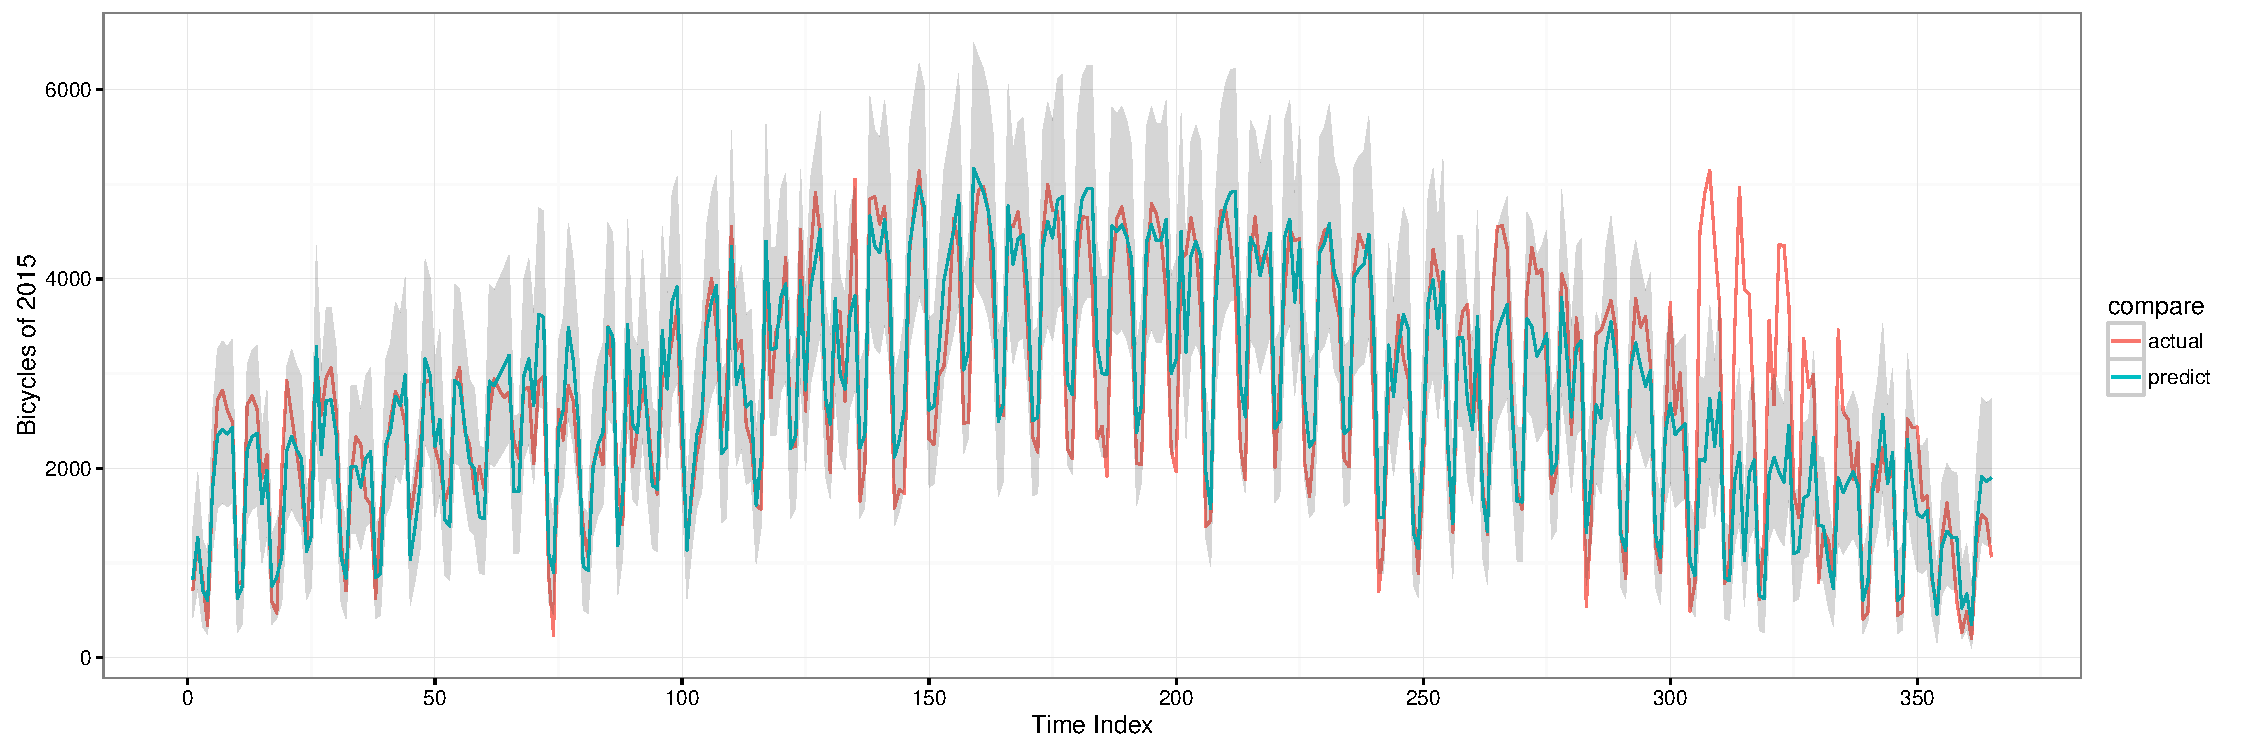
\includegraphics[width=1\textwidth]{figures/prediction/predbytime_arima} 
  \caption{Plot of actual and predicted counts for 2015 test data with 95\% predcition limits.}
  \label{fig:arimapredict}
\end{figure*}

\begin{figure*}
   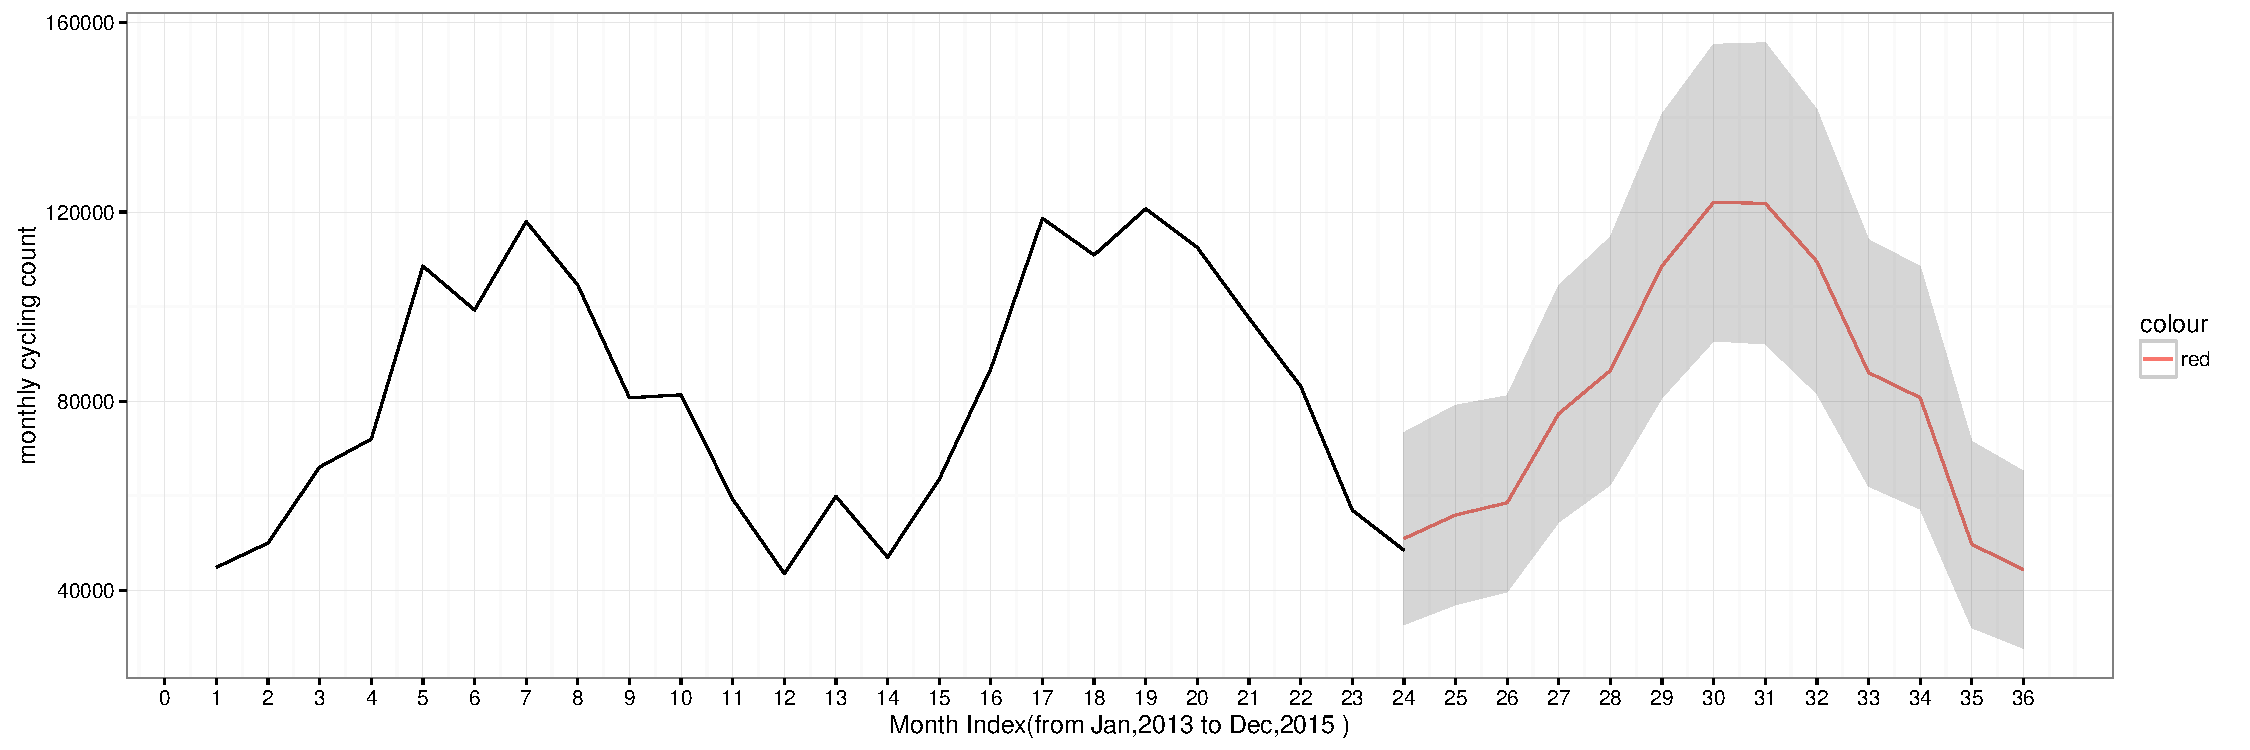
\includegraphics[width=1\textwidth]{figures/prediction/pred_month} 
  \caption{Forecast of the bike counts aggregated by month.}
  \label{fig:arimamonth}
\end{figure*}


% % Table created by stargazer v.5.2 by Marek Hlavac, Harvard University. E-mail: hlavac at fas.harvard.edu
% % Date and time: Tue, Apr 26, 2016 - 18:04:46
% % Requires LaTeX packages: dcolumn 
% \begin{table}[!htbp] \centering 
%   \caption{Results} 
%   \label{} 
% \begin{tabular}{@{\extracolsep{5pt}}lD{.}{.}{-3} D{.}{.}{-3} } 
% \\[-1.8ex]\hline 
% \hline \\[-1.8ex] 
%  & \multicolumn{2}{c}{\textit{Dependent variable:}} \\ 
% \cline{2-3} 
% \\[-1.8ex] & \multicolumn{1}{c}{poisson (Bike Counts)} & \multicolumn{1}{c}{count} \\ 
% \\[-1.8ex] & \multicolumn{1}{c}{(1)} & \multicolumn{1}{c}{(2)}\\ 
% \hline \\[-1.8ex] 
%  temperatureMaxSq & -0.0004^{***}$ $(0.00000) & -0.0004^{***}$ $(0.00000) \\ 
%   temperatureMax & 0.067^{***}$ $(0.0005) & 0.062^{***}$ $(0.001) \\ 
%   holiday & -0.266^{***}$ $(0.003) & -0.573^{***}$ $(0.005) \\ 
%   precipProbability & -0.585^{***}$ $(0.002) & -0.449^{***}$ $(0.002) \\ 
%   Wknd & -0.325^{***}$ $(0.001) & -0.731^{***}$ $(0.002) \\ 
%   daylight & 0.056^{***}$ $(0.0003) & 0.036^{***}$ $(0.0004) \\ 
%   uw & 0.113^{***}$ $(0.001) & 0.131^{***}$ $(0.001) \\ 
%   locationBGT & -0.885^{***}$ $(0.001) &  \\ 
%   locationelliott & -0.853^{***}$ $(0.001) &  \\ 
%   locationI90 & -1.398^{***}$ $(0.002) &  \\ 
%   locationSpokanebrdg & -1.243^{***}$ $(0.001) &  \\ 
%   Constant & 4.752^{***}$ $(0.015) & 5.211^{***}$ $(0.017) \\ 
%  \hline \\[-1.8ex] 
% Observations & \multicolumn{1}{c}{3,586} & \multicolumn{1}{c}{1,157} \\ 
% Log Likelihood & \multicolumn{1}{c}{-236,483.600} & \multicolumn{1}{c}{-63,703.540} \\ 
% Akaike Inf. Crit. & \multicolumn{1}{c}{472,991.200} & \multicolumn{1}{c}{127,423.100} \\ 
% \hline 
% \hline \\[-1.8ex] 
% \textit{Note:}  & \multicolumn{2}{r}{$^{*}$p$<$0.1; $^{**}$p$<$0.05; $^{***}$p$<$0.01} \\ 
% \end{tabular} 
% \end{table} 

% \subsection{Validation of the predicative model}
% \textbf{WIP-AVP, cross validation, both in-sample and out-of-sample, mse, etc).}
% In this section, we are interested to evaluate the predicative power of the two models under consideration: Model 0~\eqref{}, and the ARIMA model~\eqref{}.

% First of all, we use the entire 3 years' data to train the model and plot the actual data against fitted values, as in Figure~\ref{fig:avp_fitted}.

% Second, we use the first 2 years' data to train the model and then use the trained model to predict the 3rd year's bike counts. The actual vs predicted values plots are shown in Figure~\ref{fig:avp_crossvalidate}

%\begin{figure*}
%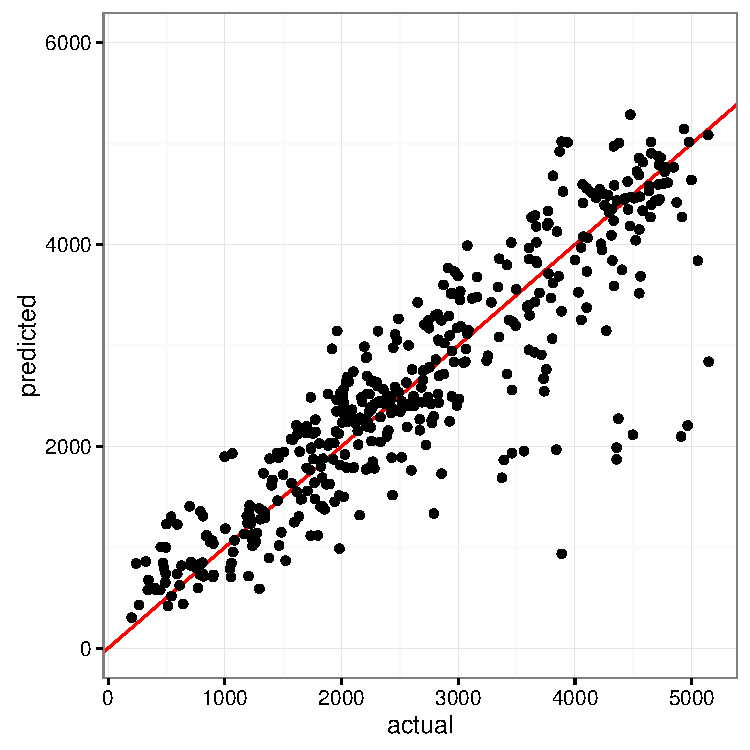
\includegraphics[width=1\textwidth]{figures/actualvspred.pdf}
%\caption{Actual vs predicted plots}
%\label{fig:avp_fitted}
%\end{figure*}

%\begin{figure*}
%%\vspace{-40pt}
%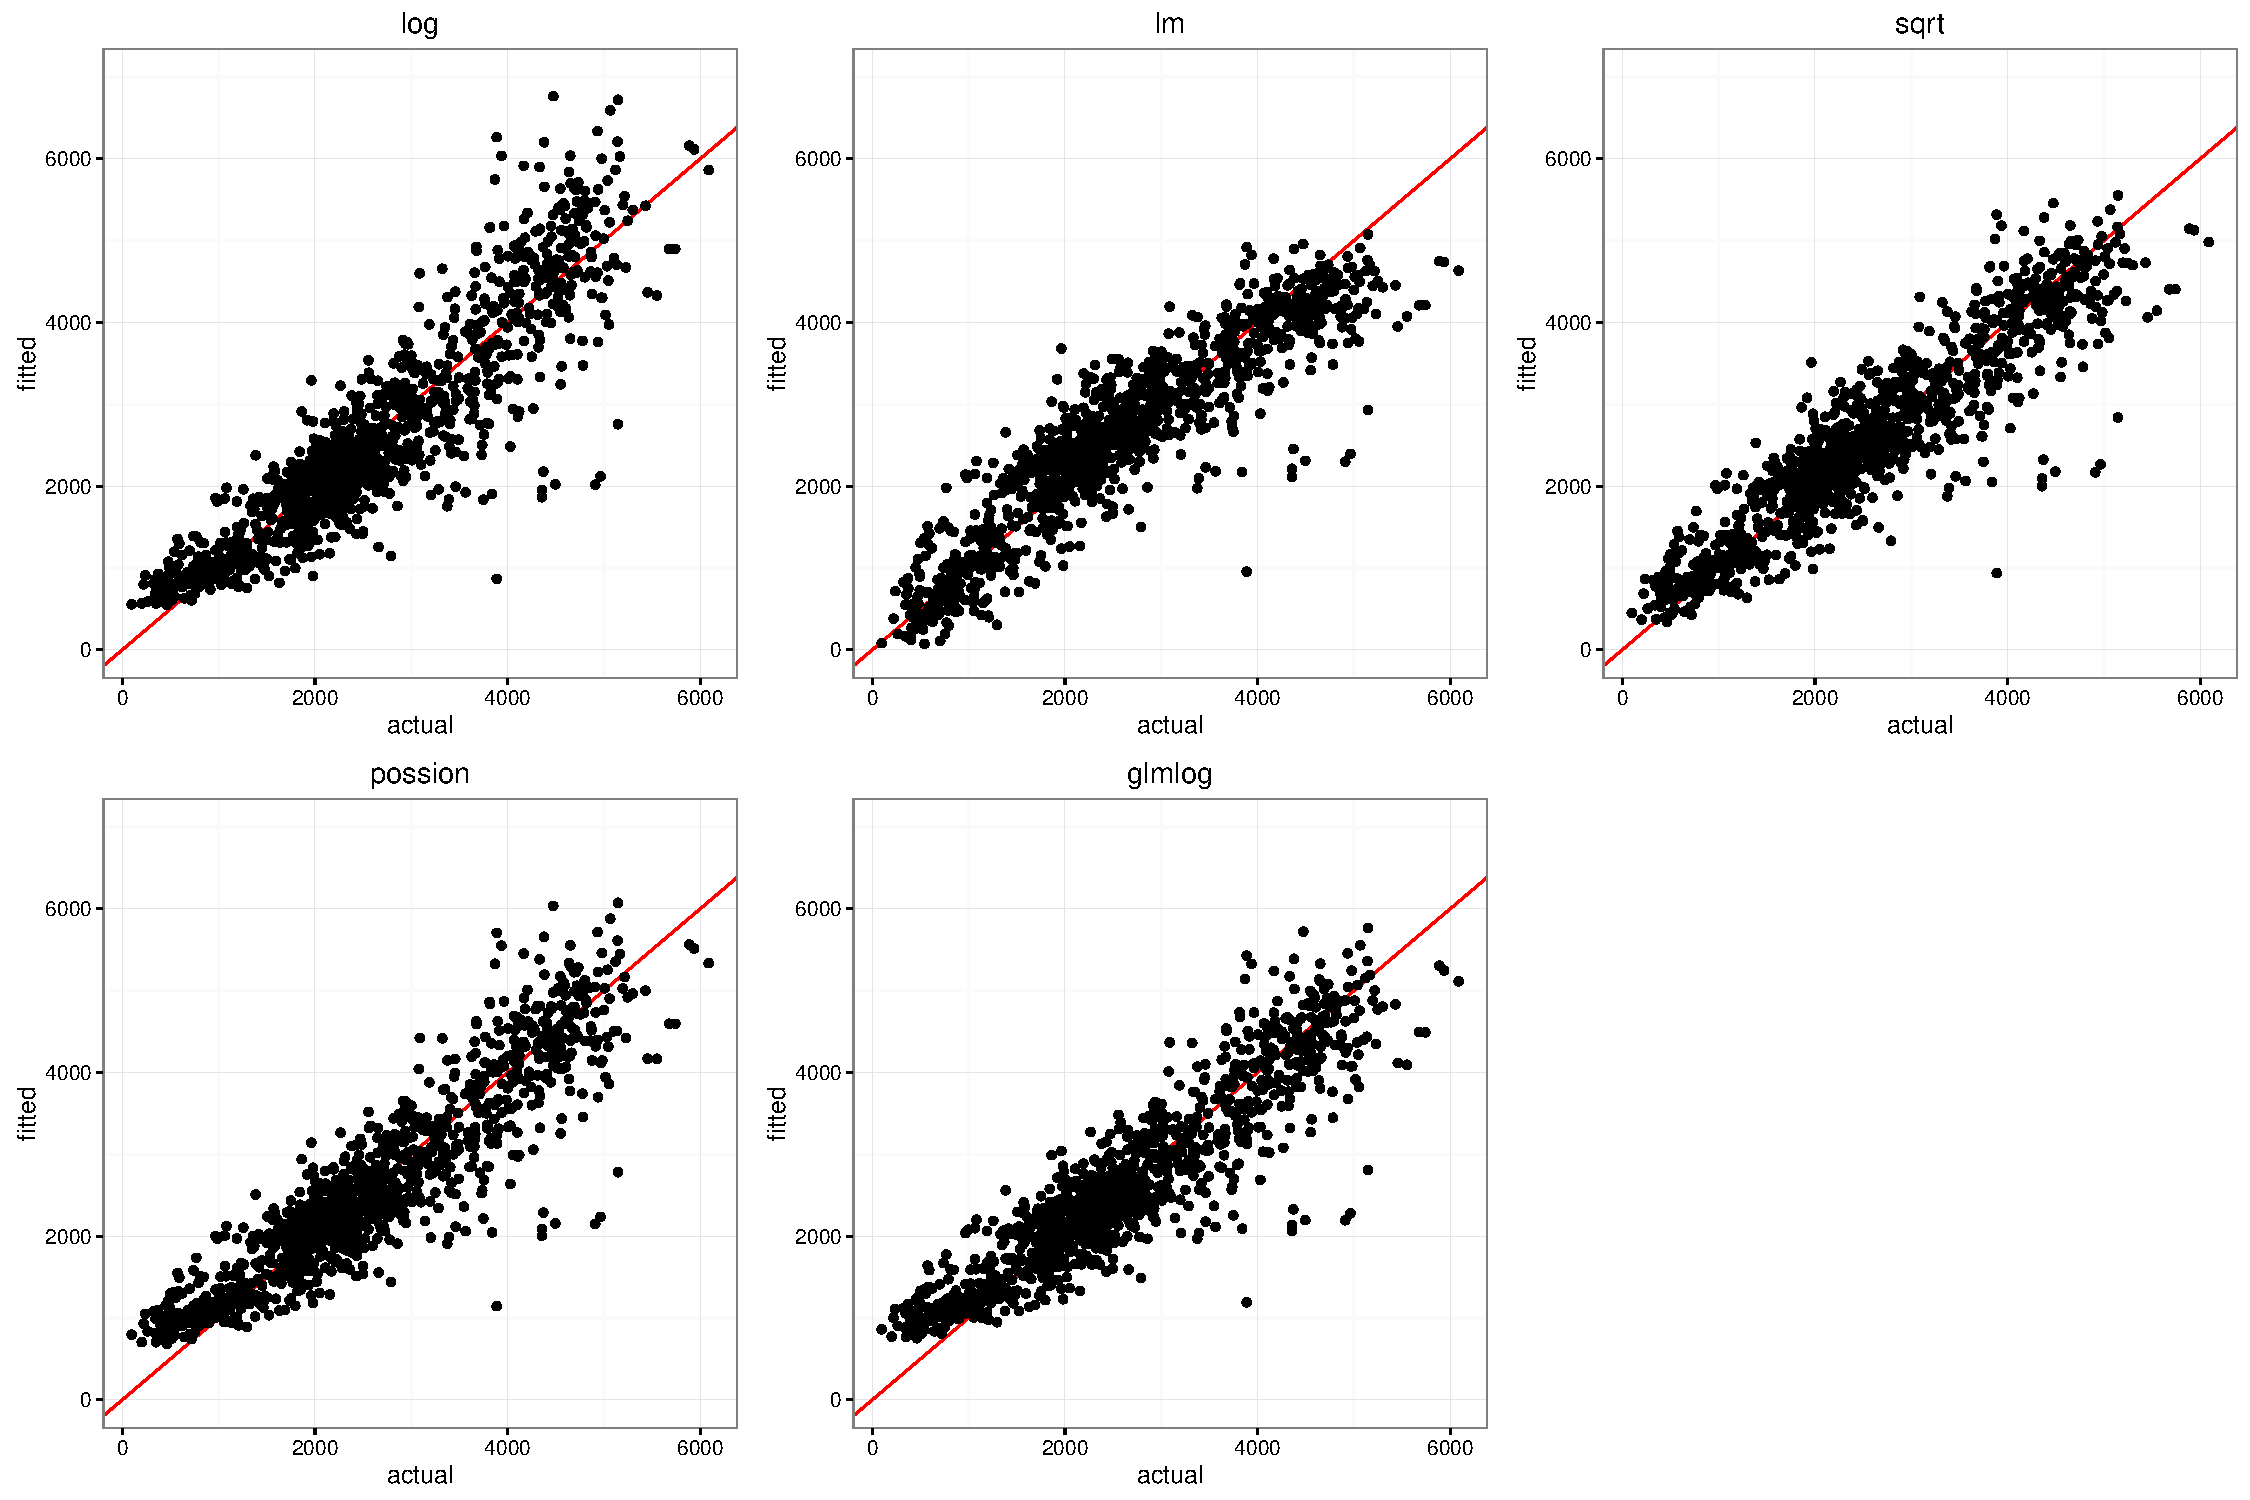
\includegraphics[width=1\textwidth]{figures/actualvsfited.pdf}
%\caption{Actual vs fitted plots}
%\label{fig:avp_crossvalidate}
%\end{figure*}

% For comparison of the predicative power, we also include the arima model for the lm model as well. See Figure~\ref{fig:avp_arima1} for cross validation and Figure~\ref{fig:avp_arima2} for fitted values.


%\begin{figure*}
%   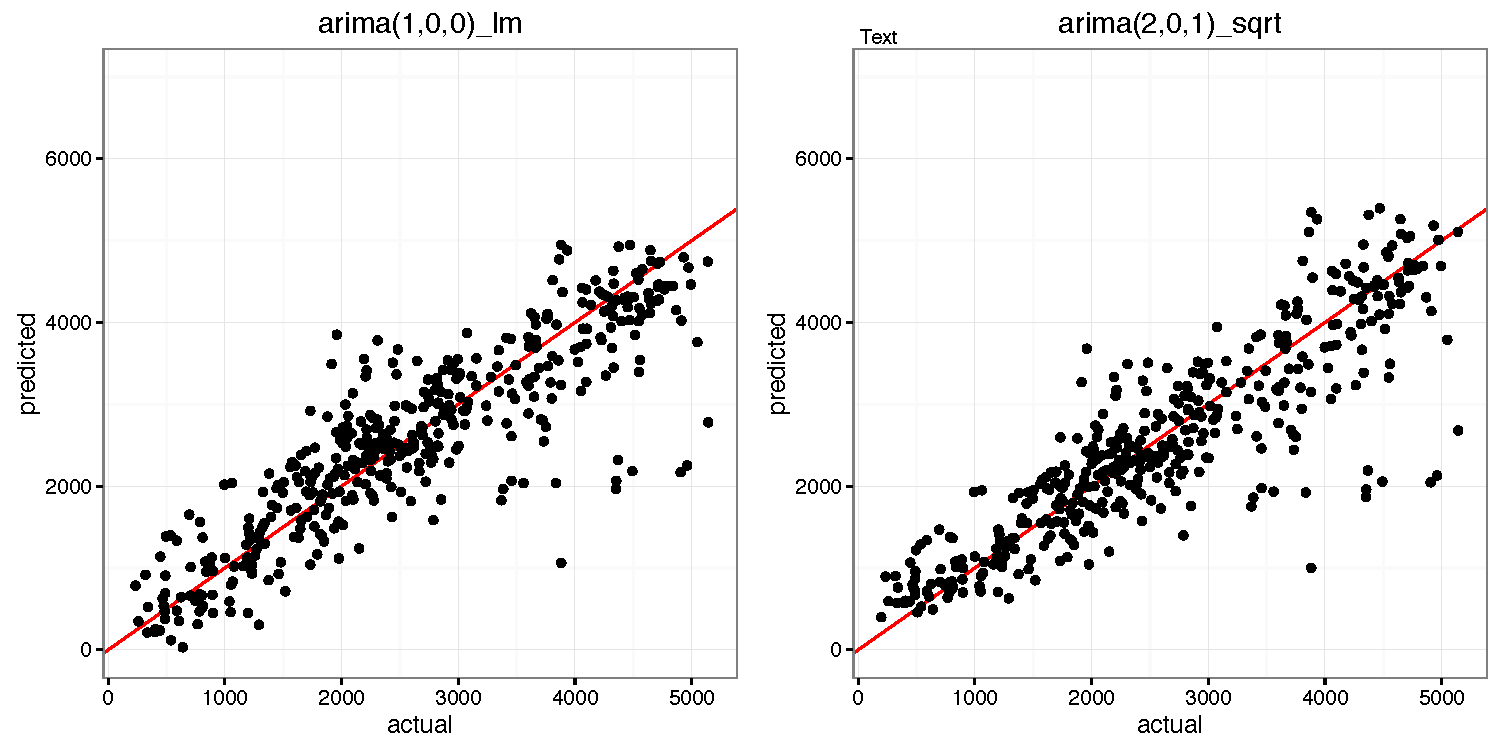
\includegraphics[width=1\textwidth]{figures/actualvspred_arima} 
%  \caption{Actual vs Predicted plots}
%  \label{fig:avp_arima1}
%\end{figure*}
%
%\begin{figure*}
%   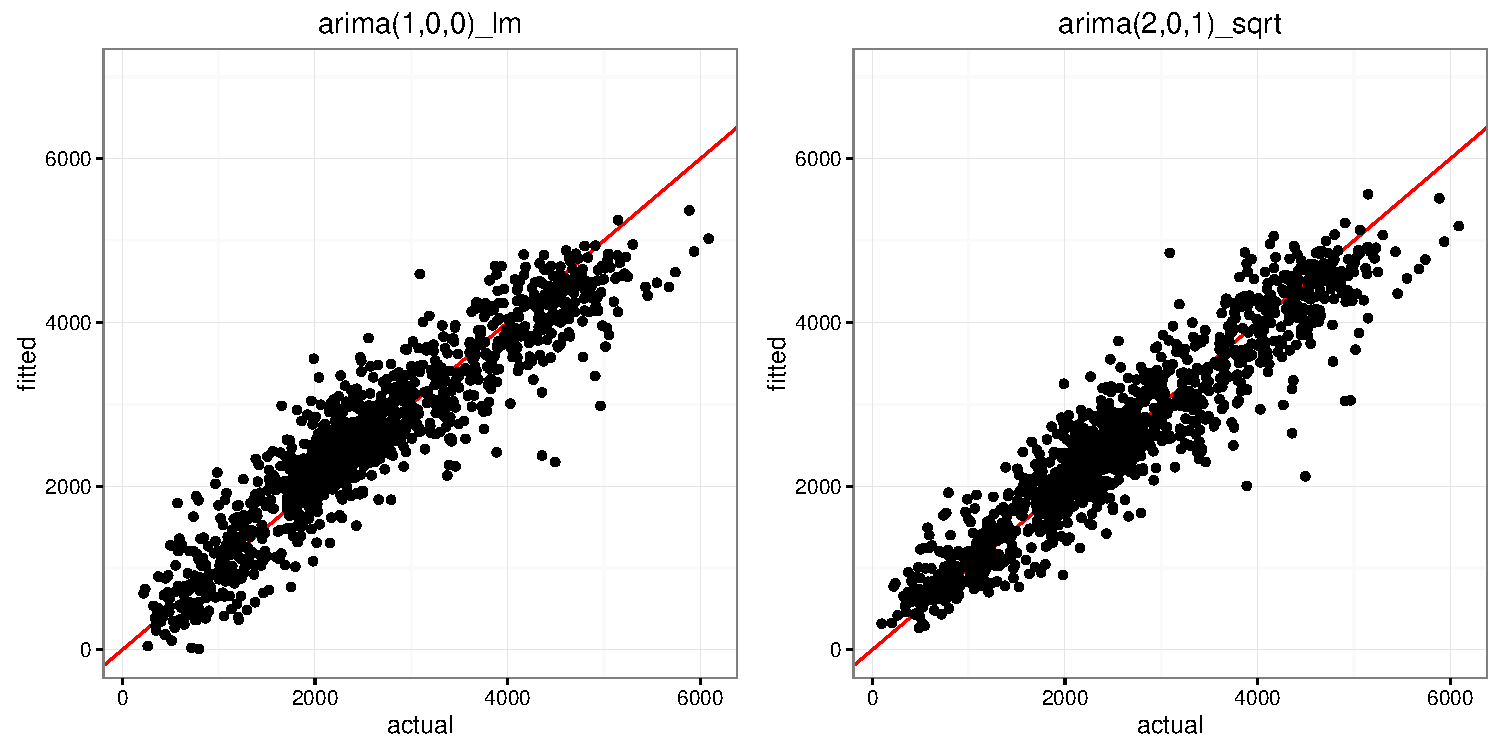
\includegraphics[width=1\textwidth]{figures/actualvsfit_arima.pdf} 
%  \caption{Actual vs Fitted plots}
%  \label{fig:avp_arima2}
%\end{figure*}

% \begin{figure}
% \centering
%   
\includegraphics[width=0.9\textwidth]{figures/prediction/actualvsfited_arima} 
%   \caption{}
%   \label{fig:arima1}
% \end{figure}

%\begin{figure}
%\centering
%   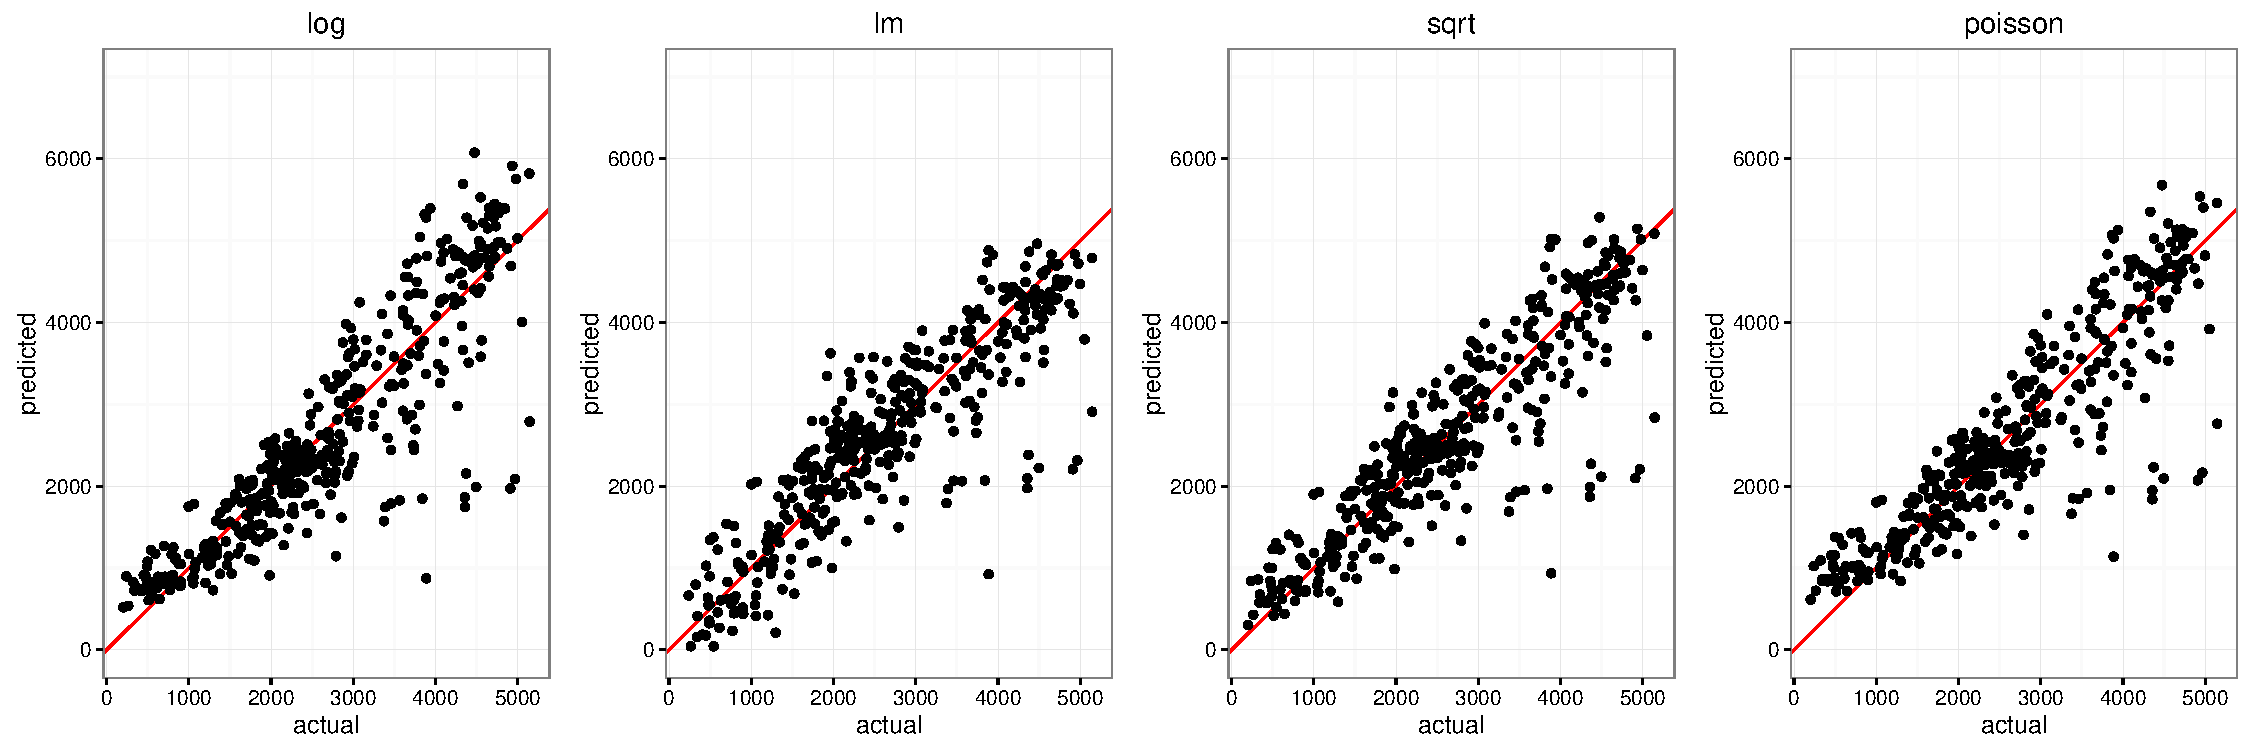
\includegraphics[width=0.9\textwidth]{figures/prediction/actualvspred4} 
%  \caption{}
%  \label{fig:arima2}
%\end{figure}


\newpage
\thispagestyle{empty}
\mbox{}


%\section{Trend Analysis}
%
%\begin{figure*}
%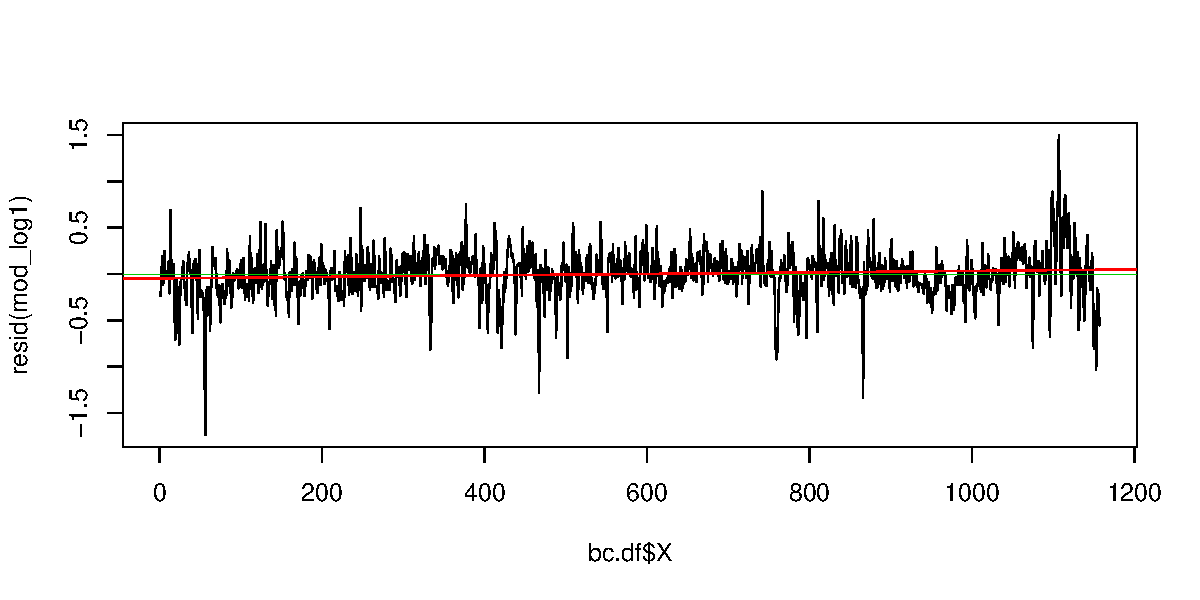
\includegraphics[width=1\textwidth]{figures/trend}
%\caption{Bike count trend after removing weather and seasonal factors. Note the green line is zero, red line is the linear model fit to the residual error of log model.}
%\label{fig:trend}
%\end{figure*}
%
%We are also interested to reveal trend from the data. More specifically, we want to ask this question: after removing all weather and seasonality factors, does the bike count have an upward trend in the past three years? To answer this question, we fit a linear model to the residual of the log model. As is shown in Figure~\ref{fig:trend}, there is a slight upward trend of the bike count in the past three years. Since we are looking at the residual error, the weather and other seasonal factors have already been removed. The red line (linear fit to the residual) has a positive slope indicates the bike count is increasing. However, such increase is very small considering the noise in daily bike count.


% ========== Chapter 5

\chapter{Conclusion and future directions}

Cycling is now becoming an increasingly important mode in a comprehensive transportation system for its physical, social, environmental and economic benefits. The city of Seattle has a vision to design and implement bicycle facilities that are safe and appropriate for riders of all ages and abilities. To achieve this goal, it's crucial for the government stakeholders, policy makers and transportation planners to understand the factors that could drive the bike demand and their predicative impact on bike travel behaviour. This thesis seeks to contribute to our limited and opaque knowledge on this topic.


The first contribution of this work is to thoroughly investigate the relationship between daily bicycle ridership with a set of key variables, including weather conditions and seasonal factors. The bike count data is continuously collected at the Fremont Bridge in Seattle for the past three years. It is joined with the daily weather conditions and other seasonal variables to form a rich modeling data set. A systematic analysis is conducted to identify explanatory variables and their appropriate forms should be included in the final model. A regression model is then proposed to adequately capture the relationship between various factors and bike counts. This study, like similiar studies on this topic, confirms that weather conditions and seasonal factors have important impact on bike volumes. The maximum daily temperature and precipitation probability is found to have the most significant effect on bicycle traffic counts. Holiday and Weekend are found to have negative impact on daily ridership. This could be explained by the fact that the bike facility under consideration is mainly utilitarian and less bike traffic is expected during holidays and weekend. With UW in session, more bike traffic will be expected possibly due to the facility's proximity to the University of Washington. Daylight hour, which serves as an indicator of the seasonality, takes account for the variations observed in different seasons. The model coefficients are reported in Table~\ref{tbl:modelresult_weather}-\ref{tbl:modelresult_interaction}, as well as visually interpreted in Figure~\ref{fig:smooth}-\ref{fig:interact}.

One of the major contributions of this work however lies in the nonlinear relationship between temperature/precipitation and bike count which is explicitly modelled and accounted for using the general additive mixture (GAM) model. The squared temperature which is commonly used in the literature can be straightforwardly justified by the smooth function of temperature obtained by the GAM model. In addition, a piecewise linear model for the precipitation probability is recommended by the GAM model. This results confirms that extreme high temperature could reduce bike volumes. It also suggests that utilitarian bikers commuting on Fremont Bridge are likely to be insensitive to rainfall unless the raining probability is very high.

With the exception of~\cite{Gallop:2012aa,Nosal:2014aa}, no other known research has studied the autocorrelation patterns in the bike count data. This research offers an ARIMA-type time series analysis model to account for the autocorrelation in the daily bike volumes, whereas hourly autocorrelation is considered in~\cite{Gallop:2012aa,Nosal:2014aa}. The proposed model is used to predict future bike volumes and its predicative performance is evaluated using the train-test framework. One potential use of the ARIMA model is to assist planners by predicting potential bike traffic fluctuation in case of inclement weather and special events, therefore better accomodate the choices cyclists make under such conditions. 

Future research directions include a further investigation on the relationship between built environment and bike ridership. Factors such as facility accessibility and bike network connectivity are expected to have significant impact on people's choice of cycling. A study on this could potentially shed light to future planning of the bike facilities and funding allocation. Also, while control of the weather and seasons are admittedly beyond the scope of policy makers,
this research does suggest that planners and policy makers may want to develop strategies that help mitigate the impacts of the natural environment during the winter months. In other words, the delta between warm dry days and cold wet days should be treated as the opportunity frontier. Future research could focus on determining what, if any, programmatic or built interventions could ameliorate unfavorable cold- and wet-weather bicycling conditions.


%
% ==========   Bibliography
%
\bibliographystyle{plain}
\bibliography{bikecounts.bib}

%
% ==========   Appendices
%
\appendix
\raggedbottom\sloppy
 
% ========== Appendix A
 
\chapter{Where to find the files}
 

\vita{Jim Fox is a Software Engineer with UW Information Technology at the University of Washington.
His duties do not include maintaining this package.  That is rather
an avocation which he enjoys as time and circumstance allow.

He welcomes your comments to {\tt fox@uw.edu}.
}


\end{document}
